%%%%%%%%%%%%%%%%%%%%%%%%%%%%%%%%%%%%%%%%%
% Arsclassica Article
% LaTeX Template
% Version 1.1 (1/8/17)
%
% This template has been downloaded from:
% http://www.LaTeXTemplates.com
%
% Original author:
% Lorenzo Pantieri (http://www.lorenzopantieri.net) with extensive modifications by:
% Vel (vel@latextemplates.com)
%
% License:
% CC BY-NC-SA 3.0 (http://creativecommons.org/licenses/by-nc-sa/3.0/)
%
%%%%%%%%%%%%%%%%%%%%%%%%%%%%%%%%%%%%%%%%%

%----------------------------------------------------------------------------------------
%	PACKAGES AND OTHER DOCUMENT CONFIGURATIONS
%----------------------------------------------------------------------------------------

\documentclass[
10pt, % Main document font size
a4paper, % Paper type, use 'letterpaper' for US Letter paper
oneside, % One page layout (no page indentation)
%twoside, % Two page layout (page indentation for binding and different headers)
headinclude,footinclude, % Extra spacing for the header and footer
BCOR5mm, % Binding correction
]{scrartcl}

%%%%%%%%%%%%%%%%%%%%%%%%%%%%%%%%%%%%%%%%%
% Arsclassica Article
% Structure Specification File
%
% This file has been downloaded from:
% http://www.LaTeXTemplates.com
%
% Original author:
% Lorenzo Pantieri (http://www.lorenzopantieri.net) with extensive modifications by:
% Vel (vel@latextemplates.com)
%
% License:
% CC BY-NC-SA 3.0 (http://creativecommons.org/licenses/by-nc-sa/3.0/)
%
%%%%%%%%%%%%%%%%%%%%%%%%%%%%%%%%%%%%%%%%%

%----------------------------------------------------------------------------------------
%	REQUIRED PACKAGES
%----------------------------------------------------------------------------------------

% Extra Visit command
\usepackage[german]{babel}

% Other commands
\usepackage[
nochapters, % Turn off chapters since this is an article        
beramono, % Use the Bera Mono font for monospaced text (\texttt)
eulermath,% Use the Euler font for mathematics
pdfspacing, % Makes use of pdftex’ letter spacing capabilities via the microtype package
dottedtoc % Dotted lines leading to the page numbers in the table of contents
]{classicthesis} % The layout is based on the Classic Thesis style

\usepackage{arsclassica} % Modifies the Classic Thesis package

\usepackage[T1]{fontenc} % Use 8-bit encoding that has 256 glyphs

\usepackage[utf8]{inputenc} % Required for including letters with accents

\usepackage{graphicx} % Required for including images
\graphicspath{{Figures/}} % Set the default folder for images

\usepackage{enumitem} % Required for manipulating the whitespace between and within lists

\usepackage{lipsum} % Used for inserting dummy 'Lorem ipsum' text into the template

\usepackage{subfig} % Required for creating figures with multiple parts (subfigures)

\usepackage{amsmath,amssymb,amsthm} % For including math equations, theorems, symbols, etc

\usepackage{varioref} % More descriptive referencing

%----------------------------------------------------------------------------------------
%	THEOREM STYLES
%---------------------------------------------------------------------------------------

\theoremstyle{definition} % Define theorem styles here based on the definition style (used for definitions and examples)
\newtheorem{definition}{Definition}

\theoremstyle{plain} % Define theorem styles here based on the plain style (used for theorems, lemmas, propositions)
\newtheorem{theorem}{Theorem}

\theoremstyle{remark} % Define theorem styles here based on the remark style (used for remarks and notes)

%----------------------------------------------------------------------------------------
%	HYPERLINKS
%---------------------------------------------------------------------------------------

\hypersetup{
%draft, % Uncomment to remove all links (useful for printing in black and white)
colorlinks=true, breaklinks=true, bookmarks=true,bookmarksnumbered,
urlcolor=webbrown, linkcolor=RoyalBlue, citecolor=webgreen, % Link colors
pdftitle={}, % PDF title
pdfauthor={\textcopyright}, % PDF Author
pdfsubject={}, % PDF Subject
pdfkeywords={}, % PDF Keywords
pdfcreator={pdfLaTeX}, % PDF Creator
pdfproducer={LaTeX with hyperref and ClassicThesis} % PDF producer
}

% -----------------------------------------------------------
% ------------ VISIT NEW COMMANDS AND PACKAGES --------------
% -----------------------------------------------------------

\usepackage[style=alphabetic,backend=bibtex,bibencoding=ascii]{biblatex} %for inline citations
\addbibresource{Bibs/baumgaertner.bib}
\addbibresource{Bibs/berndl2.bib}
\addbibresource{Bibs/kufstein.bib}
\addbibresource{Bibs/schlenker.bib}

% Koelli's commands
\newcommand{\q}[1]{``#1''}
\newcommand{\qq}[1]{`#1'} % Include the structure.tex file which specified the document structure and layout

\hyphenation{Fortran hy-phen-ation} % Specify custom hyphenation points in words with dashes where you would like hyphenation to occur, or alternatively, don't put any dashes in a word to stop hyphenation altogether

%----------------------------------------------------------------------------------------
%	TITLE AND AUTHOR(S)
%----------------------------------------------------------------------------------------

\title{\normalfont\spacedallcaps{ViSIT - Technische Dokumentation}} % The article title

%\subtitle{Subtitle} % Uncomment to display a subtitle

\author{Tobias Baumg\"artner\textsuperscript{1} \& Emanuel Berndl\textsuperscript{2} \& \\ Robert Kathrein\textsuperscript{3} \& Kris Raich\textsuperscript{3} \& \\ Florian Schlenker\textsuperscript{4}} % The article author(s) - author affiliations need to be specified in the AUTHOR AFFILIATIONS block

\date{\today} % An optional date to appear under the author(s)

%----------------------------------------------------------------------------------------

\selectlanguage{german}
\begin{document}

%----------------------------------------------------------------------------------------
%	HEADERS
%----------------------------------------------------------------------------------------

\renewcommand{\sectionmark}[1]{\markright{\spacedlowsmallcaps{#1}}} % The header for all pages (oneside) or for even pages (twoside)
%\renewcommand{\subsectionmark}[1]{\markright{\thesubsection~#1}} % Uncomment when using the twoside option - this modifies the header on odd pages
\lehead{\mbox{\llap{\small\thepage\kern1em\color{halfgray} \vline}\color{halfgray}\hspace{0.5em}\rightmark\hfil}} % The header style

\pagestyle{scrheadings} % Enable the headers specified in this block

%----------------------------------------------------------------------------------------
%	TABLE OF CONTENTS & LISTS OF FIGURES AND TABLES
%----------------------------------------------------------------------------------------

\maketitle % Print the title/author/date block

\setcounter{tocdepth}{2} % Set the depth of the table of contents to show sections and subsections only

\begin{figure}[htb]
    \centering
    
\includegraphics[scale=0.2]{Figures/general/ViSIT_Logo}
\end{figure}

\begin{figure}[htb]
    \centering
    
\includegraphics[width=\textwidth]{Figures/logos/Logo_INTEREG}
\end{figure}

\newpage

\tableofcontents % Print the table of contents

\listoffigures % Print the list of figures

\listoftables % Print the list of tables

%----------------------------------------------------------------------------------------
%	ABSTRACT
%----------------------------------------------------------------------------------------

%\section*{Abstract} % This section will not appear in the table of contents due to the star (\section*)

%\lipsum[1] % Dummy text

%----------------------------------------------------------------------------------------
%	AUTHOR AFFILIATIONS
%----------------------------------------------------------------------------------------
\begingroup
\let\thefootnote\relax\footnotetext{\textsuperscript{1} \textit{TODO, Universität Passau}}

\let\thefootnote\relax\footnotetext{\textsuperscript{2} \textit{Lehrstuhl für verteilte Informationssysteme und Data Science, Universität Passau}}

\let\thefootnote\relax\footnotetext{\textsuperscript{3} \textit{TODO, FH Kufstein}}

\let\thefootnote\relax\footnotetext{\textsuperscript{4} \textit{Forwiss, Universität Passau}}
\endgroup
%----------------------------------------------------------------------------------------

\newpage % Start the article content on the second page, remove this if you have a longer abstract that goes onto the second page

%----------------------------------------------------------------------------------------
%	INTRODUCTION
%----------------------------------------------------------------------------------------

\section{Einleitung}\label{sec:einleitung}

blub

\section{Installationsprozess}\label{sec:installationsprozess}

\subsection{Infrastruktur}

Die ViSIT-Applikationen basieren auf der Server-Client-Architektur. Damit diese Applikationen installiert werden können, wird ein hausinternes Netzwerk (Intranet) und ein damit verbundener Server - lokaler Applikations-Server (kurz LAS) - benötigt. Die ViSIT-Applikationen sind in diesem Zusammenhang die Clients, welche über das Netzwerk mit dem lokalen Applikations-Server verbunden sind. Auf dem LAS ist das ViSIT-System installiert, welches über das Internet Zugang zum globalen ViSIT-Netzwerk hat.
Das ViSIT-System ist eine Ansammlung von mehreren kleinen Applikationen, welche parallel auf dem LAS laufen können. Jeder Client, auf welchem eine der ViSIT-Applikationen läuft, hat eigene Server-Software, welche auf dem LAS installiert ist und für die serverseitigen Berechnungen zuständig ist.

Die Applikationen wurden mit der IT-Technologie “Docker” erstellt. Mit Docker hat man die Möglichkeit, Anwendungen in sogenannten Containern auszuführen und diese Container können aufeinander aufbauen und miteinander kommunizieren. Im Gegensatz zu einer virtuellen Maschine, ist eine Docker-basierte Anwendung nur ein Prozess, der auf dem System ausgeführt wird. Es ist somit kein Gastbetriebssystem erforderlich, wie dies bei Virtuellen Maschinen der Falls ist. Container sind einfach konfigurierbare, abgeschlossene Einheiten, in welchen die Anwendung ausgeführt werden. 
Mit Docker können Linux-Container erstellt und verwendet werden können. Die erstellten Container sind eine Virtualisierung auf der Ebene des Betriebssystems. Durch das Erstellen von Containern, werden isolierte Linux-Systeme auf dem gleichen Host erzeugt. Diese Container können flexibel erstellt, bereitgestellt, kopiert und zwischen Umgebungen verschoben werden. Zweck dieser Container ist die Unabhängigkeit und die Fähigkeit, mehrere Prozesse und Applikationen getrennt voneinander betreiben zu können. Die Vorteile von Docker-Containern sind unter anderem Modularität und Versionsverwaltung. Modularität ermöglicht es, bei zum Beispiel einer Reparatur oder Aktualisierung einer Applikation, nur einen Teil dieser Applikation außer Betrieb zu nehmen, ohne die gesamte Applikation außer Betrieb nehmen zu müssen. Docker bietet eine eingebaute Versionsverwaltung, welche es erlaubt, den aktuellen Stand eines Containers in ein sogenanntes Image zu sichern. Somit ist es möglich, die unterschiedlichen Zustände eines Images in einer Historie nachzuverfolgen. Ein Image ist ein Speicherabbild eines Containers und es besteht aus mehreren Layern, welche schreibgeschützt sind und somit nicht verändert werden können. Ein Layer ist wiederum ein Teil eines Images und enthält einen Befehl oder eine Datei, welche dem Image hinzugefügt wurde. Aufgrund dieser Layer kann die ganze Historie eines Images nachvollzogen werden.

\subsection{Projekt auf dem LAS installieren}

Als erster Schritt muss die Datenbank für die Applikation angelegt werden. Wie oben erklärt, wurde für das ViSIT-Projekt Docker verwendet. Damit gespeicherte Daten auch außerhalb eines Containers abgelegt oder in einem anderen Container eingebunden werden können, werden sogenannte Volumes erstellt. Volumes haben viele Vorteile, vor allem aber sind sie einfacher zu sichern oder zu migrieren. Volumes funktionieren sowohl auf Linux- als auch auf Windows-Containern.
Im ersten Schritt wird ein Volume mit der Datenbank auf dem lokalen Rechner im Terminal mit dem Kommando
\begin{lstlisting}[style=MyBashStyle]
docker volume create visit-database
\end{lstlisting} erstellt. Einen eigenen Volume benötigt man deshalb, weil die dort abgelegten Daten permanent gespeichert werden müssen - würde z.B.: der Container gelöscht oder beendet werden - dann wären die nur im Docker Container gespeicherten Daten ebenfalls gelöscht werden. Damit dies nicht passieren kann, werden die Daten parallel lokal auf dem Rechner gespeichert.
Damit Dateien zwischen Geräten in einem lokalen Netzwerk oder zwischen entfernten Geräten über das Internet synchronisiert werden können, wird eine Datensynchronisation mit Peer-to-Peer-Übertragung benötigt. Dies wird im ViSIT-Projekt mit Syncthing realisiert und auch dafür muss ein eigener Volume lokal auf dem Rechner erstellt werden. Dies geschieht mit \begin{lstlisting}[style=MyBashStyle]
docker volume create visit-syncthing
\end{lstlisting}-Befehl, welcher ebenfalls im Terminal ausgeführt wird.
Als nächster Schritt wird das gesamte ViSIT-Projekt von GitHub mittels

\begin{lstlisting}[style=MyBashStyle]
docker run -d --name visit -p 80:80 -p 22000:22000 -p 21027:21027
-v visit-syncthing:/var/syncthing
-v s:/p2p/visit:/var/p2p
-v visit-database:/var/lib/mysql
--restart unless-stopped visitapp/maincontainer \end{lstlisting}

geklont. Beim erstmaligen Starten benötigt der Vorgang länger, da das Projekt aus dem Git Repository sowie das Appbundle (https://github.com/ViSIT-Dev/appbundle) heruntergeladen werden.\\

Erklärung der einzelnen Befehle:\\
\begin{lstlisting}[style=MyBashStyle]
docker run -d --name visit -p 80:80 -p 22000:22000 -p 21027:21027 
\end{lstlisting}


docker run startet den Container und mit den mit den Parametern -d gibt man an, dass der Container im Hintergrund dauerhaft laufen soll (Daemonmode). Weiters wird mit --name visit der Name des Containers festgelegt, in diesem Fall heißt der Container visit. Der Container kann im weiteren Verlauf auch über diesen Namen angesprochen werden.
Mit dem Parameter -p 80:80 werden die Ports vom Host an den Container gebunden. Hier wird der lokale Hostport 80 auf den Containerport 80 gemappt. Die weiteren Ports -p 22000:22000 -p 21027:21027 werden für das Syncthing und für das Peer to Peer-Netzwerk benötigt.
Als nächstes folgt der Befehl -v visit-syncthing:/var/syncthing. Mit dem Parameter -v wird ein Verzeichnis (Volume) auf dem Hostrechner zu einem Verzeichnis innerhalb des Containers verbunden, auf diese Weise werden die Daten persistent gespeichert, das heißt, dass ein Ordner auf dem Hostsystem auf einen Ordner im Container gemappt wird. Das bedeutet, dass die Daten in beiden Ordnern immer inhaltsgleich sind. Ohne dem Mapping zu einen Ordner auf dem Hostsystem, wären alle Daten aus dem Docker Container, wenn dieser Container gelöscht wird, ebenfalls gelöscht. Um die Daten persistent, also dauerhaft zu speichern, wird immer ein Ordner im Hostsystem mit dem entsprechenden Ordner im Docker Container gemappt.
Zuerst wird das Verzeichnis auf dem Hostrechner angegeben, hier visit-syncthing, und nach dem Doppelpunkt steht das Verzeichnis innerhalb des Containers, hier /var/syncthing. 
Im nächsten Teil des Befehls -v s:/p2p/visit:/var/p2p wird ebenfalls zuerst das Verzeichnis auf dem Hostrechner angegeben, s:/p2p/visit und dann das Verzeichnis innerhalb des Containers /var/p2p.
Im nächsten Befehl -v visit-database:/var/lib/mysql geht es um die Verbindung zur Datenbank. Hier wird ebenfalls zuerst das Verzeichnis auf dem Hostrechner angegeben visit-database und nach dem Doppelpunkt steht das Verzeichnis innerhalb des Containers /var/lib/mysql.
Zuletzt wird mittels --restart unless-stopped visitapp/maincontainer dem System mitgeteilt, dass der Docker Container visitapp/maincontainer automatisch gestartet werden soll außer, wenn er manuell oder anderweitig gestoppt wird.

Wenn der Vorgang abgeschlossen ist, kann über Lokalhost im Browser unter localhost:80/typo3/ das Backend aufgegerufen werden. Das erstmalige einloggen in das Backend (TYPO3) erfolgt mit dem Benutzername: admin und Passwort: visit-admin.


\cite{anno4j1}

\section{Tobi - App Framework}\label{sec:appframework}

TODO rename label and heading

\cite{anno4j2}

\section{Kompression}\label{sec:compression}

\subsection{Motivation}

Unabhängig davon, ob man eine Ausstellung in einem Museum gestaltet oder eine Webseite erstellt, lässt sich fast jede für Besucher oder Benutzer konzipierte Darstellung durch den Einsatz von Bildern aufwerten. Dieses lässt sich durch den Einsatz von 3D-Modellen, mit welchen der Benutzer durch Drehen, Zoomen, etc. interagieren kann, noch deutlich steigern. Abgesehen davon, dass dies in einer Ausstellung nur durch den Einsatz von Rechnern, wie beispielsweise von Tablets, möglich ist, sind damit jedoch einige technische Herausforderungen verbunden.

Einerseits erwartet der Benutzer ein möglichst realistisches Erlebnis, was nur durch hochaufgelöste 3D-Modelle und den damit einhergehenden großen Datenmengen möglich ist. Dennoch soll das Modell möglichst ohne Latenz angezeigt werden und flüssige Interaktion erlauben. Soll die Darstellung darüber hinaus auf einem mobilen Endgerät des Benutzers, wie beispielsweise einem Smartphone, stattfinden, das einerseits nur eingeschränkte Rechenkapazität bietet und auf das andererseits die gesamten Daten für jeden Benutzer separat übertragen werden müssen, entsteht hier ein Gegensatz, für den ein geeigneter Kompromis zu finden ist.

Dieser Kompromis besteht darin, die 3D"=Modelle nicht in der höchsten verfügbaren Auflösung dem Benutzer darzustellen, sondern in einer dem Anwendungsfall und dem Endgerät angemessenen Größe. Beispielsweise ist für eine ansprechende Anzeige auf einem Smartphone"=Bildschirm eine geringere Auflösung notwendig als auf der Workstation eines Museumsmitarbeiters mit entsprechend großem Bildschirm, die auch dementsprechend leistungsfähig ist, und über welche dieser Mitarbeiter das angezeigte Objekt erforschen möchte. Aus diesem Grund ist es sinnvoll, die gespeicherten 3D"=Modelle in verschiedenen Auflösungen in der Medien-Datenbank bereit zu halten, weshalb diese in der Regel beim Hochladen in die Datenbank automatisch komprimiert werden.

Die eben beschriebene Problematik tritt nicht nur bei 3D"=Modellen auf, sondern auch bei herkömmlichen zweidimensionalen Bildern. Da auch solche Medien in der Medien"=Datenbank gespeichert werden sollen, sind auch Bilddateien zu komprimieren, was sich sehr einfach durch das Verringern der Auflösung bewerkstelligen lässt. Von jedem hochgeladenen Bild werden also komprimierte Versionen in verschiedenen Auflösungsstufen erstellt, auf welche anschließend zugegriffen werden kann.

In diesem Kapitel wird nach einer kurzen Erläuterung der theoretischen Grundlagen auf die an die ViSIT"=Medien"=Datenbank angebundene Kompressions"=Komponente und deren Voraussetzungen, ihre Funktionsweise, die Installation und die Bedienung, die über eine Web-Oberfläche erfolgt, eingegangen. Außerdem werden die zur Verfügung stehenden Konfigurationsoptionen eingehend erläutert. Abschließend wird die Schnittstelle (API), über welche die Kompressions"=Komponente unabhängig von der dafür verfügbaren Web-Oberfläche oder der ViSIT"=Medien"=Datenbank angesprochen werden kann, spezifiziert.

\subsection{Grundlagen}

Bei 3D-Modellen gilt es grundsätzlich zwischen der Geometrie, durch welche die Form der Oberfläche eines Objekts beschrieben wird, und der Textur, durch welche die Färbung der Oberfläche ausgedrückt wird, zu unterscheiden. Während die Geometrie obligatorisch für ein 3D-Modell ist, muss nicht zwangsläufig eine Textur existieren. Nicht jedes Digitalisierungsverfahren ist in der Lage, Texturdaten zu erfassen, so beispielsweise ein Laserscanner. Im Folgenden werden Aufbau und Kompression dieser beiden Bestandteile eines 3D-Modells behandelt.

\subsubsection{Geometrie von 3D-Modellen}
\label{schlenke:chp:fundamentalsGeometry}

Herkömmliche 3D"=Modelle, die ausschließlich die Oberfläche eines Objekts und nicht dessen Inneres beschreiben, bestehen aus mehreren Punkten im dreidimensionalen Raum, die \emph{Vertices} genannt werden. Diese Punkte werden zu Flächen, den sogenannten \emph{Faces} verbunden, wobei es sich hier in vielen Fällen um Dreiecke handelt. Die Anzahl der Ecken eines Faces wird als dessen \emph{Ordnung} bezeichnet. Die Kanten dieser Flächen, die Verbindungen zwischen zwei Vertices darstellen, werden \emph{Edges} genannt. Die Gesamtheit aller Vertices und Faces eines 3D"=Modells wird auch als \emph{Mesh} bezeichnet. Die soeben genannten Begriffe werden in \autoref{schlenke:fig:fundamentals:geo} grafisch dargestellt.

\begin{figure}
\centering
\subfloat[Vertex]{
\includegraphics[width=0.25\textwidth]{Figures/schlenker/fundamentals/basicVertex.png}}
\qquad
\subfloat[Edge]{
\includegraphics[width=0.25\textwidth]{Figures/schlenker/fundamentals/basicEdge.png}}
\qquad
\subfloat[Face]{
\includegraphics[width=0.25\textwidth]{Figures/schlenker/fundamentals/basicFace.png}}\\
\subfloat[Mesh]{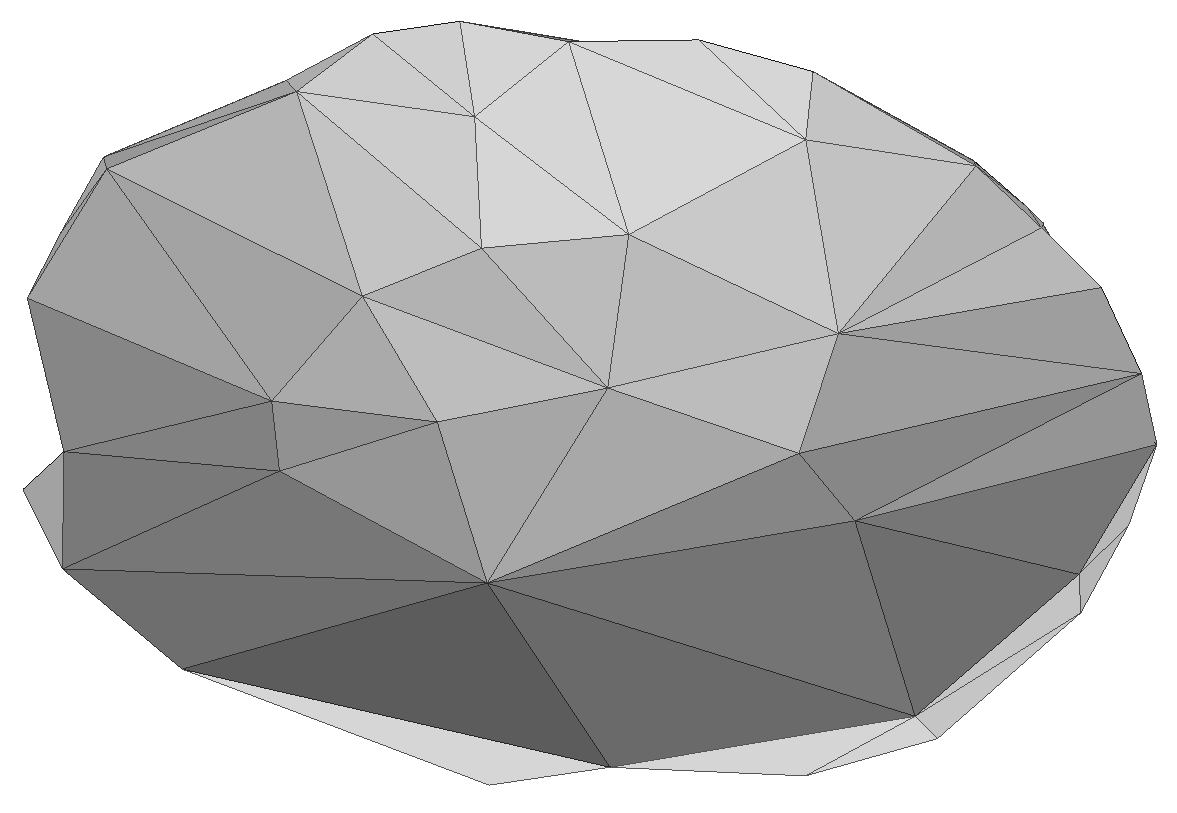
\includegraphics[width=0.70\textwidth]{Figures/schlenker/fundamentals/basicMesh.png}}
\caption{Grundlegende Elemente der Geometrie eines 3D-Modells}
\label{schlenke:fig:fundamentals:geo}
\end{figure}

Während bei einfachen Dateiformaten, wie beispielsweise dem STL-Format\footnote{\url{http://www.fabbers.com/tech/STL_Format}}, für jedes Face die Koordinaten eines jeden Eckpunkts separat gespeichert werden, wird die dadurch verursachte Redundanz zum Beispiel bei OBJ-Dateien\footnote{\url{http://www.martinreddy.net/gfx/3d/OBJ.spec}} vermieden, indem zunächst alle Vertices in Form der Koordinaten einmalig angegeben werden und anschließend bei der Definition der Faces auf diese Vertexdefinition indexbasiert zugegriffen wird.

Bei Meshes, die ein reales Objekt beschreiben, sollte dieser möglichst einer orientierbaren stetigen zweidimensionalen Mannigfaltigkeit, die in den dreidimensionalen Raum eingebettet ist, entsprechen \cite[S.~3]{botsch2010}. Dies hat zur Folge, dass für jeden Punkt im Raum eindeutig entschieden werden kann, ob er im Inneren oder im Äußeren des Objekts liegt. Dies impliziert beispielsweise, dass kein Edge Teil von mehr als zwei Faces sein kann. Jedoch sind auch an die Vertices bestimmte Bedingungen zu stellen, wobei für Details auf \cite[S.~11f]{botsch2010} verwiesen wird.

\subsubsection{Textur von 3D-Modellen}

Die Textur eines 3D"=Modells beschreibt dessen Färbung der Oberfläche, wodurch ihr eine äußerst wichtige Bedeutung für das visuelle Erlebnis beim Betrachten des Modells zukommt. Sie wird in der Regel getrennt von den eigentlichen Geometriedaten in einer separaten Bild"=Datei gespeichert. Für jedes Face wird dann durch die sogenannten \emph{Texturkoordinaten} festgelegt, welcher Ausschnitt des Textur-Bildes auf diesem Dreieck angezeigt wird. Pro Face werden also für jeden Eckpunkt zwei Werte gespeichert, durch welche eine eindeutige Position im Bild definiert wird. Da in der Regel bei den meisten Vertices alle angrenzenden Faces die gleichen Texturkoordinaten verwenden, wird dieses Paar von Werten beispielsweise bei OBJ-Dateien nur einmal gespeichert, worauf anschließend bei der Beschreibung der Faces indexbasiert zugegriffen wird.

Manchem Leser stellt sich hier die Frage, ob generell die Verwendung von einem Paar Texturkoordinaten pro Vertex, welches dann für alle angrenzenden Faces verwendet wird, nicht ausreichend wäre. Hier spielt jedoch die Geometrie des 3D"=Modells, genauer deren \emph{Topologie}, eine wichtige Rolle. Entspricht diese einer (verzerrten) Ebene, so wäre diese Vereinfachung in der Tat ausreichend. Betrachtet man aber beispielsweise eine Kugel, so lässt sich das zweidimensionale Bild nicht über die Kugel legen, ohne dass eine Kante entsteht, an welcher mindestens zwei Ränder des Bildes aneinandergrenzen. Genau entlang dieser Linie, dem sogenannten \emph{Texture Seam}, befinden sich dann die Vertices, für welche je nach angrenzendem Face verschiedene Texturkoordinaten verwendet werden müssen. Unabhängig von der soeben dargelegten Notwendigkeit dieser Texture Seams lässt sich durch eine sinnvolle Unterteilung der Textur auch die Qualität erhöhen, indem für alle Bereiche des 3D"=Modells eine ähnliche Auflösung verwendet wird und durch starke Streckungen oder Stauchungen verursachte Verzerrungen der Textur auf dem Modell minimiert werden.

\subsubsection{Kompression der Geometrie}
\label{schlenke:chp:fundamentals:geocomp}

Eine der wichtigsten Herangehensweisen zur Kompression von 3D"=Modellen ist die Reduktion von Vertices und damit einhergehend die Verringerung der Anzahl an Faces. Ausgehend von einem hoch aufgelösten Modell mit einer hohen Anzahl an Vertices ist die auf den ersten Blick einfachste Vorgehensweise das Entfernen eines möglichst unwichtigen Vertices. Das dadurch entstehende Loch im Mesh muss anschließend geschlossen werden. Dadurch entsteht jedoch im Allgemeinen ein Face mit einer höheren Ordnung, was oft unerwünscht ist. In diesem Fall muss das entstehende Loch mit Dreiecken gefüllt werden, wofür es keine eindeutige und daher auch unterschiedlich gute Lösungen gibt. Stattdessen verwenden viele Kompressionsverfahren, wie auch der in dieser Kompressions-Komponente verwendete Algorithmus, sogenannte \emph{Edge-Collapse}-/\emph{Half-Edge-Collapse}-Operationen.

Bei einer solchen Edge-Collapse-Operation, wie sie in Abbildung \ref{schlenke:fig:fundamentals:edgecollapse} dargestellt ist, werden zwei durch ein Edge verbundene Vertices zu einem neuen Vertex verschmolzen. Dabei degenerieren die an dieses Edge angrenzende Faces und werden entfernt. Zusätzlich lassen sich neben dem kontrahierten Edge noch weitere Edges entfernen. Entspricht der Mesh lokal einer Mannigfaltigkeit, werden durch eine Edge-Collapse-Operation also zwei Faces, drei Edges und ein Vertex entfernt. Vor dem Durchführen einer derartigen Operation muss jedoch überprüft werden, ob die in \cite[S.~118f]{botsch2010} erläuterte \emph{Link Condition} erfüllt ist, da andernfalls die Topologie des Meshes durch die Operation verändert werden kann. Entspricht der neue Vertex einem der beiden ursprünglichen Vertices, so spricht man von einem Half-Edge-Collapse.

\begin{figure}
\centering
\subfloat[Situation vor der Operation]{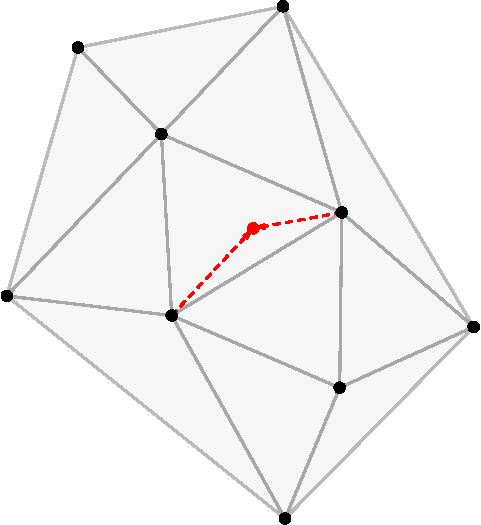
\includegraphics[width=0.45\textwidth]{Figures/schlenker/fundamentals/edgeCollapseACropped.pdf}}
\qquad
\subfloat[Situation nach der Operation]{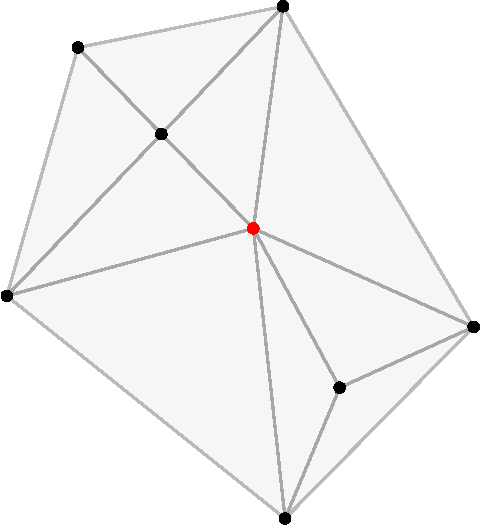
\includegraphics[width=0.45\textwidth]{Figures/schlenker/fundamentals/edgeCollapseBCropped.pdf}}
\caption{Beispiel einer Edge-Collapse-Operation. Die Zielposition der beiden an das Edge angrenzenden Vertices ist \emph{rot} markiert.}
\label{schlenke:fig:fundamentals:edgecollapse}
\end{figure}

Es verbleibt jedoch die Frage, welche Paare von Vertices verschmolzen werden sollen. Hierfür wird in \cite{garland1997} ein Verfahren vorstellt, das mithilfe von Quadriken jeder möglichen Edge-Collapse-Operation einen Wert für die damit verbundenen Kosten zuweist. Iterativ werden nun die Vertices aus Operationen mit den geringsten Kosten verschmolzen, woraufhin die Kosten der Operationen, die sich auf die umliegenden Vertices beziehen, aktualisiert werden müssen.

Der Algorithmus aus \cite{garland1997} ist jedoch nur auf nicht-texturierte Meshes anwendbar. Möchte man dieses Verfahren verwenden, um 3D"=Modelle mit Textur zu komprimieren, so müssen einerseits die Verschmelzungsoperationen auch auf die Texturkoordinaten angewandt werden, was insbesondere entlang von Texture Seams eine sehr sorgfältige Implementierung erfordert, andererseits müssen aber auch diese Texturkoordinaten in die Berechnung der Kosten für die jeweilige Operation miteinbezogen werden. Abweichungen in der resultierenden Oberfläche des 3D"=Modells haben hier Verzerrungen in der Textur zur Folge. Dies gilt auch für Texture Seams, bei welchen es darüber hinaus nicht vermeiden lässt, dass auch Bereiche der als Textur verwendeten Bilddatei für die Einfärbung der Faces verwendet werden, die im ursprünglichen Modell überhaupt nicht parametrisiert waren und somit beliebigen Inhalt aufweisen können. Es empfiehlt sich daher, die Ränder der Bereiche in der Bilddatei mit einem ähnlichen Farbton wie die eigentliche Textur zu färben, was bei den meisten Textur erzeugenden Programmen automatisch geschieht. Die daher notwendige Erweiterung des bestehenden Kompressions-Algorithmus auf texturierte Meshes wird in \cite{garland1998} vorgenommen, wobei Texture Seams dort kaum behandelt werden. Die für die Kompressions-Komponente erstellte Implementierung behandelt jedoch auch diese Bereiche auf eine sinnvolle Art und Weise.

\subsubsection{Kompression der Textur}

Während die Kompression der Modellgeometrie insbesondere bei texturierten Meshes nichttrivial ist, gestaltet sich die Kompression der Texturdaten relativ einfach. Die Textur wird in einer herkömmlichen Bilddatei gespeichert, deren Dateigröße direkt von der Auflösung des darin gespeicherten Bildes abhängt. Wird die Auflösung des Bildes verringert, was der Funktionsumfang eines jeden brauchbaren Bildbearbeitungsprogramms zulässt, schlägt sich dies auch in der Größe der Texturdatei nieder. Darüber hinaus sind weitere aus der Bildverarbeitung bekannte Kompressionsverfahren einsetzbar, wie zum Beispiel die JPEG-Komprimierung\footnote{https://www.ece.ucdavis.edu/cerl/reliablejpeg/compression/}.

Allerdings muss darauf geachtet werden, dass die zusammen mit der Modellgeometrie gespeicherten Texturkoordinaten auch nach der Kompression der Textur wohldefiniert sind. Besonders angenehm ist hier jedoch die Tatsache, dass diese Texturkoordinaten sich nicht auf die Pixel beziehen, sondern stets im Interval von null bis eins liegen, wobei sich null auf den oberen bzw. linken Rand und eins auf den unteren bzgl. rechten Rand der Texturdatei bezieht. Aus diesem Grund sind die Texturkoordinaten gänzlich unabhängig von der Auflösung der die Textur beinhaltenden Bilddatei und diese Datei kann ohne Modifizierung der Geometriedatei komprimiert werden. Diese Aussage gilt nicht nur für die Anpassung der Auflösung, sondern auch für andere Kompressionsverfahren aus der Bildverarbeitung.

\subsection{Voraussetzungen}

Die Kompressions-Komponente dient zur Kompression von Mediendaten, die im Dateimanagement auf dem Lokalen Anwendungsserver (LAS) registriert sind. Die Kompressions"=Komponente läuft innerhalb eines separaten Docker"=Containers auf dem Server, wofür die Software Docker\footnote{\url{https://www.docker.com/}} auf dem als Host"=System fungierenden Server installiert sein muss. Eine direkte Interaktion des Benutzers mit der Kompressions"=Komponente findet in der Regel nicht statt. Es wird jedoch eine Web"=Oberfläche zur Administration und Konfiguration des Systems bereitgestellt. 

Da die zu komprimierenden Dateien auf dem Host"=System gespeichert sind, worauf sowohl von der Medien"=Datenbank als auch von der Kompressions"=Komponente zugegriffen wird, ist es nicht möglich, das Kompressions"=System unabhängig von der Medien"=Datenbank auszuführen. Andernfalls würden in der Medien"=Datenbank hochgeladene Dateien der Kompressions"=Komponente nicht zur Verfügung stehen. 

\subsubsection{Hardwarevoraussetzungen}
\label{schlenke:chp:info:hardware}

Die Anforderungen an die Ressourcen, die sich für den LAS bzw. den Docker"=Container der Kompressions"=Komponente ergeben, hängen in erster Linie von der Größe der zu komprimierenden Mediendateien ab. Während die Prozessorleistung primär die Dauer der Kompressions"=Prozesse bedingt, beschränkt der zur Verfügung stehende Arbeitsspeicher die maximale Größe der Eingabedaten nach oben.
Da der Algorithmus zur Kompression von 3D-Modellen kaum Parallelisierungs"=Möglichkeiten bietet, werden die Berechnungen derzeit nicht auf mehrere Prozessorkerne oder auf die Grafikkarte verlagert. 
Experimente während der Implementierung haben gezeigt, dass Modelle mit ca. 8 Mio. Dreiecken auf einem aktuellen gut ausgestatteten Bürorechner (Intel-Core-i7-Prozessor, 32 GB RAM) komprimiert werden können. Da insbesondere der Arbeitsspeicher der limitierende Faktor ist, spielt jedoch der Speicherbedarf der anderen auf dem System laufenden Anwendungen eine wichtige Rolle.

\subsubsection{Softwarevoraussetzungen}

Die Kompressions-Komponente wurde in der Programmiersprache Java implementiert, weshalb zur Ausführung ein Java Runtime Environment (JRE) im Docker-Container installiert sein muss. Für die Kompression von Bild- und Texturdateien wird im Hintergrund die Software ImageMagick verwendet. Es ergeben sich also die folgenden beiden Software-Abhängigkeiten:
\begin{itemize}
\item Java Runtime Environment\footnote{\url{https://java.com/de/download/}} (getestet mit Version 1.8.0)
\item ImageMagick\footnote{\url{https://imagemagick.org/index.php}} (getestet mit Version 7.0.8)
\end{itemize}
Da diese Software"=Produkte jedoch bei der Installtion des entsprechenden Docker"=Containers automatisch installiert werden, muss dies nicht manuell durch den Benutzer vollzogen werden. 

\subsubsection{Abgrenzungskriterien}

Das Absetzen eines Kompressions-Auftrags wird in der Regel von der Medien"=Datenbank"=Komponente angestoßen. Dennoch wird eine Benutzeroberfläche zum manuellen Absetzen von Kompressions"=Aufträgen zur Verfügung gestellt, die jedoch aufgrund der Notwendigkeit der manuellen Angabe von Identifikatoren keinen hohen Bedienkomfort bietet.

An Medientypen werden Bilder und 3D-Modelle unterstützt. Andere Medientypen können mit dieser Komponente nicht komprimiert werden. An Bilddaten können alle Bildformate komprimiert werden, die von der Software ImageMagick unterstützt werden. An 3D"=Modellen können texturierte und nicht-texturierte Modelle komprimiert werden, die im OBJ"=Format\footnote{\url{http://www.martinreddy.net/gfx/3d/OBJ.spec}} gespeichert werden. Andere Dateien müssen zunächst manuell durch Drittsoftware in das OBJ-Format übersetzt werden. Pro Modell ist aufgrund von Limitierungen in der Medien"=Datenbank maximal eine Material- und eine Texturdatei zulässig. Genauere Informationen über die für ein 3D"=Modell notwendigen und möglichen Dateien sind in folgender \autoref{schlenke:tbl:3d-files} dargestellt. Der implementierte Algorithmus wäre jedoch prinzipiell in der Lage, auch Objekte mit mehreren Texturdateien zu komprimieren.

\begin{table}
\begin{center}
{\footnotesize
\begin{tabular}{llll}
Dateiendung & Informationen & Optional & Notwendigkeit \\
\hline
.obj & Geometriedaten & Nein & Genau eine Datei erforderlich \\
.mtl & Materialdefinitionen & Ja & Maximal eine Datei möglich \\
.jpg/.jpeg/.png & Texturdaten & Ja & Maximal eine Datei, nur falls auch \\
& & & MTL-Datei spezifiziert wird \\
\end{tabular}}
\caption{Für ein 3D"=Modell notwendige und optionale Dateien}
\label{schlenke:tbl:3d-files}
\end{center}
\end{table}

Die in Abschnitt \ref{schlenke:chp:info:hardware} benannten Hardware"=Voraussetzungen gilt es zu beachten.

Bei 3D-Modellen wird vorausgesetzt, dass die Eingabedaten den Voraussetzungen mannigfaltigen Meshes, wie sie in Abschnitt \ref{schlenke:chp:fundamentalsGeometry} beschrieben wurden, genügen. Für Modelle, welche diese Eigenschaft nicht aufweisen, wird keine Garantie bezüglich des Ergebnisses des Kompressionsvorgangs gegeben. Mögliche Konsequenzen sind ein Fehlschlagen des Kompressionsvorgangs oder unbrauchbare Resultate, auch wenn ein Fehlschlagen in den Experimenten nicht beobachtet wurde. Das Eingabemodell sollte möglichst ausschließlich aus Dreiecken bestehen. Faces höherer Ordnung werden beim Einlesen naiv in Dreiecke umgewandelt, wobei auch hier keine Garantie bezüglich der Qualität des Ergebnisses gegeben werden kann. 

Eine Darstellung der Eingangsdaten oder deren komprimierter Versionen findet innerhalb der Kompressions"=Komponente nicht statt. Die Resultate des Kompressionsvorgangs werden lediglich als Datei im System abgelegt.

Die Kompressions"=Komponente bietet keinerlei Benutzerauthentifizierung oder sonstige Zugriffsbeschränkungen. Die Komponente muss anderweitig vor dem Zugriff Dritter geschützt werden. Für den Zugriff auf die API und die Konfigurations- und Administrationsoberfläche kann lediglich eine Whitelist mit IP"=Adressen hinterlegt werden, für welche der Zugriff exklusiv gewährt wird.

\subsection{Funktionsweise}
\label{schlenke:chp:funktionsweise}

Die Kompressions"=Komponente dient zum Abarbeiten von Kompressions"=Aufträgen, wobei letztere die Kompression \emph{einer} medialen Repräsentation eines Objekts in \emph{mehreren} Auflösungsstufen umfasst. Die Medien"=Dateien stehen dem Kompressions"=System über das Dateisystem zur Verfügung. In der Regel wird ein Kompressions"=Auftrag direkt nach dem Hochladen einer Medien"=Datei in die ViSIT"=Medien"=Datenbank abgesetzt.

Bei der Abarbeitung eines Kompressions"=Auftrags werden zunächst die technischen Metadaten aus der Meta"=Datenbank abgerufen. Diese technischen Metadaten werden für jede mediale Repräsentation gespeichert und umfassen wichtige Informationen über die dazugehörigen Medien"=Dateien und die bestehenden Kompressionsstufen. Sie können außerdem Kontext"=Informationen über eine mediale Repräsentation beinhalten, so speichert beispielsweise die Kompressions"=Komponente bei 3D"=Modellen die Anzahl der Vertices und der Faces. Die technischen Metadaten liegen in der Meta"=Datenbank im JSON-Format\footnote{\url{http://www.ecma-international.org/publications/files/ECMA-ST/ECMA-404.pdf}} vor, wobei hierfür die in Listing \ref{schlenke:lst:technicalMetaSpec} dargestellte Spezifikation gilt. Im Anschluss wird unterschieden, ob es sich bei der zu komprimierenden Medien"=Datei um ein Bild oder ein 3D"=Modell handelt. Ausschlaggebend hierfür ist der im Kompressions"=Auftrag angegebene MIME"=Typ.

\begin{lstlisting}[float, caption={Spezifikation des die technischen Metadaten beinhaltenden JSON-Objekts},label=schlenke:lst:technicalMetaSpec]
{
		"title"	: string,
		"description" : string,
		"objectTripleID" : string,
		"objectTripleURL" : string,
		"mediaTripleID" : string,
		"mediaTripleURL" : string,
		"MIMEtype" : string
		"createDate" : timestamp,
		"creatorID" : string,
		"creatorName" : string,
		"rightholder" : string,
		"uploader" : string, 
		"files" : {
				"origin" : {
						"uploadDate" : timestamp,
						"accessLevel" : string,
						"license" : string,
						"fileSize" : long,
						"paths" : [string],
						"fileTypeSpecificMeta" : object
				},
				...
		}
}
\end{lstlisting}

Die beiden in diesem Objekt verwendeten URLs bezeichnen die ID des Metadatums, welches durch die mediale Repräsentation beschrieben wird, in der Meta"=Datenbank ({\ttfamily object\-Triple\-URL}) bzw. die ID der digitalen Repräsentation selbst ({\ttfamily media\-Triple\-URL}), wie in Abbildung \autoref{fig:digrep} veranschaulicht wird. Diese beiden Werte haben die Form einer URL und können somit nicht als Dateinamen verwendet werden, wie es in der Medien"=Datenbank geschieht. Jedoch verwenden alle in diesem Kontext auftretenden URLs das gleiche Präfix, wodurch die Eindeutigkeit auch bei einer Beschränkung auf das Suffix gewährleistet bleibt, welches sich als Dateiname eignet. Das Suffix der {\ttfamily object\-Triple\-URL} wird als {\ttfamily object\-Triple\-ID}, das der {\ttfamily media\-Triple\-URL} als {\ttfamily media\-Triple\-ID} bezeichnet. Ein Beispiel hierzu ist in Abbildung \ref{schlenke:fig:IdAndUrlExample} zu sehen.

\begin{figure}
\[\underbrace{\mbox{\ttfamily http://visit.de/metadb/}\underbrace{\mbox{\ttfamily 7dde4f1c-022f-4489-9f13-d568ab3c7905}}_{\mbox{mediaTripleID}}}_{\mbox{mediaTripleURL}}\] 
\caption{Beziehung von mediaTripleID und mediaTripleURL anhand eines Beispiels}
\label{schlenke:fig:IdAndUrlExample}
\end{figure}

Die Dateien werden in der Medien"=Datenbank im Format
\begin{lstlisting}[caption={Schema der Dateinamen in der Medien-Datenbank, das ebenfalls durch das Kompressions-System verwendet wird}]
objectTripleID.mediaTripleID.compressionLevelID.Dateiendung
\end{lstlisting}
abgespeichert, worauf ebenfalls durch das Kompressions"=System zugegriffen wird. Hierbei bezeichnet {\ttfamily compressionLevelID} die Bezeichnung für die jeweilige Kompressions"=Stufe. Für die Originaldatei wird hierbei {\ttfamily origin} verwendet, für 3D"=Modelle die Vertexanzahl und für Bilder der in der Konfiguration festgelegte Titel für die jeweilige Auflösungsstufe.

Im folgenden wird auf die Semantik der einzelnen Werte dieses JSON-Objekts eingegangen:
\begin{itemize}
\item {\ttfamily title}: Ein vom Benutzer festgelegter Titel des Objekts
\item {\ttfamily description}: Eine vom Benutzer festgelegte Beschreibung des Objekts
\item {\ttfamily objectTripleID}: Wie oben beschrieben
\item {\ttfamily objectTripleURL}: Wie oben beschrieben
\item {\ttfamily mediaTripleID}: Wie oben beschrieben
\item {\ttfamily mediaTripleURL}: Wie oben beschrieben
\item {\ttfamily createDate}: Der UNIX-Timestamp, an dem die Datei in die Medien"=Datenbank geladen wurde
\item {\ttfamily creatorID}: Die Syncthing-ID des Netzwerkteilnehmers, von dem die Datei hochgeladen wurde
\item {\ttfamily creatorName}: Der Name des Netzwerkteilnehmers, von dem die Datei hochgeladen wurde
\item {\ttfamily rightholder}: Der Rechteinhaber an der Medien"=Datei
\item {\ttfamily uploader}: Name der Person, welche die Datei in die Medien"=Datenbank geladen hat
\item {\ttfamily MIMEtype}: MIME-Typ der Medien-Datei (z.~B. \glqq{}image/png\grqq{} für ein PNG"=Bild oder \glqq{}text/plain\grqq{} für ein 3D"=Modell)
\item {\ttfamily files}: Ein Objekt, das für jede zur Verfügung stehende Kompressions"=Stufe (inklusive der Originaldatei) weiterführende Informationen bereitstellt. Diese werden als Objekt in einer Eigenschaft gespeichert, deren Titel der Bezeichnung der jeweiligen Kompressions"=Stufe entspricht, also beispielsweise {\ttfamily origin} für die Originaldatei. Dieses Objekt weist das folgende Schema auf:
	\begin{itemize}
	\item {\ttfamily uploadDate}: Der UNIX-Timestamp, an dem diese Kompressions"=Stufe erstellt wurde
	\item {\ttfamily accessLevel}: Zugriffsberechtigung für die Kompressions"=Stufe in der Medien"=Datenbank, kann entweder {\ttfamily public}, {\ttfamily private} oder {\ttfamily visit} sein
	\item {\ttfamily license}: Lizenz, unter der die Mediendatei in dieser Kompressions"=Stufe verfügbar ist
	\item {\ttfamily fileSize}: Größe der Mediendatei in Bytes (bei 3D"=Modellen mit mehreren Dateien die Summe aller Dateien)
	\item {\ttfamily paths}: Array mit den internen Dateinamen aller zu dieser medialen Repräsentation gehöriger Dateien
	\item {\ttfamily fileTypeSpecificMeta}: Weitere unspezifizierte Informationen zu dieser Kompressions"=Stufe
	\end{itemize}
\end{itemize}

\paragraph{Bilddatei}

Zur Kompression von Bildateien wird im Hintergrund die Software ImageMagick verwendet. Für jede der in der Konfiguration festgelegten Auflösungsstufen, die kleiner als die Originalgröße des Bildes ist, wird damit eine verkleinerte Version des Bildes erstellt. Laut den technischen Metadaten bereits existierende Auflösungsstufen werden dabei übersprungen. Die neu erstellten Auflösungsstufen werden nun den technischen Metadaten hinzugefügt und in die Meta"=Datenbank überführt.

\paragraph{3D-Modell}

Ein texturiertes 3D"=Modell besteht in der Regel aus drei Dateien. Die OBJ"=Datei mit den Geometriedaten verweist auf eine MTL"=Datei, welche die Materialeigenschaften der Oberfläche beschreibt und insbesondere auf vorhandene Textur"=Dateien referenziert. Beim Hochladen eines 3D"=Modells in die Medien"=Datenbank werden die Dateien dort automatisch umbenannt. Die Referenzen, die zwischen den Dateien bestehen, werden dabei jedoch nicht angepasst und daher ungültig. Im ersten Schritt der Kompression werden diese Verweise in den Originaldateien repariert, indem sie an die neuen Dateinamen angepasst werden. Auch die zum unkomprimierten Modell gehörenden technischen Metadaten werden angepasst.

Nachdem das unkomprimierte Modell repariert wurde, kann mit der eigentlichen Kompression begonnen werden. Zunächst werden die Geometriedaten (OBJ"=Dateien) und ggf. auch die Material"=Datei komprimiert und abgespeichert, wobei auch hier laut den technischen Metadaten bereits existierende Auflösungsstufen übersprungen werden. Nachdem alle Varianten der Geometriedaten erstellt wurden, erfolgt bei texturierten Modellen die Kompression der Textur separat für jede Auflösungsstufe, erneut unter der Zuhilfenahme der Software ImageMagick. Die zuvor erstellten Material"=Dateien verweisen bereits auf die nun erstellten Bilddateien. Wie bereits bei den Bilddateien werden abschließend die um die neuen Auflösungsstufen erweiterten technischen Metadaten an die Meta"=Datenbank übertragen.

\subsection{Installation und Steuerung }

\subsubsection{Installation}

Zur Installation des Kompressions"=Systems muss zunächst über den Befehl 
\begin{lstlisting}[caption=Befehl zum Erstellen des Docker-Images]
docker build -t "visitapp/compression" https://github.com/ViSIT-Dev/compressioncontainer.git
\end{lstlisting}
ein Docker"=Image erstellt werden. Nun muss ein Verzeichnis gewählt werden, über das von außen auf die das Kompressions"=System betreffende Dateien, wie die Log"=Dateien oder die Konfiguration zugegriffen wird. Hier werde beispielsweise das Verzeichnis {\ttfamily /etc/visit-compression} gewählt. Anschließend kann über den Befehl
\begin{lstlisting}[caption=Befehl zum Erstellen des Docker-Containers]
docker run -d --name compression -p 1613:1613 -v visit-p2p-private:/var/www/Private -v /etc/visit-compression:/root/compression visitapp/compression
\end{lstlisting}
aus dem soeben erstellten Docker"=Image ein ausführbarer Docker"=Container generiert werden, sofern {visit-p2p-private} das Docker"=Volume bezeichnet, in welchem die Medien"=Dateien gespeichert sind. Die einzelnen Bestandteile dieses Befehls werden im folgenden kurz erläutert:
\begin{itemize}
\item {\ttfamily docker run}: Dies ist der Befehl zum Erstellen eines Docker"=Images.
\item {\ttfamily -d}: Der Container soll im Hintergrund ausgeführt werden.
\item {\ttfamily -p 1613:1613}: Der Port 1613 innerhalb des Docker"=Containers soll zum Host"=System durchgeschleift werden. Sollen andere Ports verwendet werden, muss dieser Bestandteil entsprechend angepasst werden.
\item {\ttfamily -v visit-p2p-private:/var/www/Private}: Das beim Einrichten der Medien"=Datenbank erzeugte Docker"=Volume {\ttfamily visit-""p2p-""private}, in dem die Medien"=Dateien gespeichert sind, soll innerhalb des Docker"=Containers unter dem Pfad {\ttfamily /var/www/Private} verfügbar sein.
\item {\ttfamily -v /etc/visit-compression:/root/compression}: Auf dem Host"=System soll unter dem Verzeichnis {\ttfamily /etc/visit"=compression} auf die Dateien zugegriffen werden können, welche sich innerhalb des Docker"=Containers im Verzeichnis {\ttfamily /root/compression} befinden.
\item {\ttfamily visitapp/compression}: Dies ist die gewählte Bezeichnung für das eben erstellte Docker"=Image.
\end{itemize}
Nach dem Erstellen des Docker"=Containers wird dieser automatisch gestartet und kann, wie im folgenden Abschnitt erläutert wird, beendet oder neu gestartet werden. Bei gestartetem Container ist die Web"=Oberfläche in der Standardkonfiguration unter \url{http://localhost:1613} erreichbar, während die API unter \url{http://localhost:1613/api} zur Verfügung steht. Bevor die Kompressions"=Komponente vollständig funktionstüchtig ist, müssen jedoch die Konfigurationsoptionen geeignet angepasst werden, wobei hierfür auf Abschnitt \ref{schlenke:chp:configuration} verwiesen wird.

\subsubsection{Steuerung des Docker-Containers}

Der die Kompressions"=Komponente beinhaltende Docker"=Container kann wie jeder andere Container mit den Befehlen
\begin{lstlisting}[caption={Kommando zum Beenden des Docker-Containers der Kompressions-Komponente},label=schlenke:lst:dockerstop]
docker stop compression
\end{lstlisting}
gestoppt und mit dem Befehl
\begin{lstlisting}[caption={Kommando zum Starten des Docker-Containers der Kompressions-Komponente}]
docker start compression
\end{lstlisting}
wieder gestartet werden. Alle Einstellungen bleiben dabei erhalten. Über das bei der Installation angegebene Verzeichnis (standardmäßig {\ttfamily /etc/visit-compression}) kann auch außerhalb des Containers auf das Kompressions"=System betreffende Dateien zugegriffen werden. So kann durch Editieren der Datei {\ttfamily config.ini} die Konfiguration angepasst werden, wobei für ein Aktivieren der aktualisierten Einstellungen ein Neustart des Docker"=Containers erforderlich ist. Außerdem kann auf die Log"=Datei {compression.log} zugegriffen werden, die insbesondere bei fehlgeschlagenen Kompressions"=Aufträgen oder bei unerwartetem Beenden des Kompressions"=Systems wichtige Informationen über die zugrunde liegende Ursache liefern kann. Da die Ausgabe dieser Informationen zusätzlich über die Standardausgabe erfolgt, besteht eine weitere Möglichkeit des Zugriffs im Ausführen des Kommandos:
\begin{lstlisting}[caption={Kommando zum Anzeigen der Ausgaben des Kompressions-Systems}]
docker logs compression
\end{lstlisting}
Für fortgeschrittene Benutzer, welche Anpassungen direkt im Docker"=Container vornehmen möchten, kann über den Befehl
\begin{lstlisting}[caption={Befehl zum Öffnen einer Kommandozeile im Kompressions-Container}]
docker exec -it compression /bin/bash
\end{lstlisting}
eine Kommandozeile geöffnet werden.

\subsubsection{Steuerung der Kompressions-Komponente}
\label{schlenke:chp:componentcontrol}

Sämtliche Kommunikation mit der Kompressions"=Komponente selbst erfolgt über die bereitgestellte API. Die zur Verfügung stehende Web"=Oberfläche greift ebenfalls über diese API auf das System zu. Für Details zur Web"=Oberfläche und zur API wird auf die Abschnitte \ref{schlenke:chp:webui} und \ref{schlenke:chp:api} verwiesen.

Die Kompressions"=Komponente startet automatisch nach dem Start des entsprechenden Docker"=Containers. Je nach Konfiguration wird daraufhin unmittelbar mit dem Abarbeiten von Kompressions"=Aufträgen begonnen. 

Die Kompressions"=Komponente lässt sich über entsprechende API"=Aufrufe in unterschiedlichen Modi herunterfahren. Diese Modi umfassen
\begin{itemize}
\item das Abarbeiten aller noch ausstehender Aufträge vor dem Beenden,
\item das Abarbeiten nur des sich aktuell in Verarbeitung befindlichen Auftrags und
\item das sofortige Beenden des Systems ohne Rücksichtnahme auf die ausstehenden Kompressions"=Aufträge.
\end{itemize} 
In jedem Fall werden keine weiteren Kompressions"=Aufträge angenommen. Ausstehende Kompressionsaufträge bleiben beim erneuten Starten der Komponente erhalten. Jedoch wird ein etwaiger Auftrag, der sich während des Beendens in der Verarbeitung befand, als \glqq{}Fehlerhaft abgeschlossen\grqq{} markiert.

Diese Methode des Herunterfahrens erlaubt im Gegensatz zum Stoppen des Docker"=Containers die kontrollierte Handhabung noch ausstehender oder sich in Verarbeitung befindlicher Kompressions"=Aufträge. Allerdings wird durch das Herunterfahren der Kompressions"=Komponente der sie enthaltende Docker"=Container nicht automatisch mit beendet. Dies muss separat durch das Kommando in \autoref{schlenke:lst:dockerstop} erfolgen. Wird der Container mit diesem Kommando ohne vorheriges Herunterfahren des Kompressions"=Systems ausgeführt, entspricht dies dem sofortigen Beenden des Systems ohne Rücksichtnahme auf die ausstehenden Kompressions"=Aufträge.

\subsection{Konfiguration}
\label{schlenke:chp:configuration}

Beim Starten des Kompressions-Systems wird automatisch eine Konfigurationsdatei mit den Standardwerten  unter dem Pfad
\begin{lstlisting}
/root/compression/config.ini
\end{lstlisting} 
angelegt, sofern eine solche nicht bereits an dieser Position existiert. Einige der Werte lassen sich nur manuell über diese Datei anpassen. Auf die wichtigsten Konfigurationsmöglichkeiten kann jedoch auch von außen über die API und die Web-Oberfläche sowohl lesend als auch schreibend zugegriffen werden. Beim manuellen Anpassen der Konfigurationsdatei muss darauf geachtet werden, dass innerhalb der Variablenwerte die Zeichen \glqq{}:\grqq{}, \glqq{}=\grqq{} und \glqq{}\textbackslash\grqq{} mit einem vorgestellten Backslash versehen werden müssen, also beispielsweise durch \glqq{}https\textbackslash ://\grqq{}. Für Details diesbezüglich wird auf die entsprechende Java-Dokumentation\footnote{\url{https://docs.oracle.com/javase/7/docs/api/java/util/Properties.html\# load(java.io.Reader)}} verwiesen. \autoref{schlenke:tbl:configOptions} gibt Aufschluss über alle Konfigurationsmöglichkeiten, welche in den folgenden Abschnitten detailliert erläutert werden.

\begin{table}
\begin{center}
%\resizebox{\textwidth}{!}{
\begin{tabular}{lll}
\hline
Variable & Standard & Web\\
\hline
\multicolumn{3}{c}{Verwaltung von Kompressionsaufträgen} \\
\hline
{\lstinline|accessWhiteListIps|} & {\lstinline|[127.0.0.1,*]|} & {\footnotesize Ja} \\
{\lstinline|apiPort|} & {\lstinline|1613|} & {\footnotesize Ja} \\
{\lstinline|archiveDisplayLength|} & {\lstinline|250|} & {\footnotesize Nein} \\
{\lstinline|autostart|} & {\lstinline|true|} & {\footnotesize Ja} \\
{\lstinline|mediaFileRootDirectory|} & {\lstinline|/var/www/private|} & {\footnotesize Nein} \\
{\lstinline|queueMaxLength|} & {\lstinline|5000|} & {\footnotesize Ja} \\
\hline
\multicolumn{3}{c}{3D-Kompression} \\
\hline
{\lstinline|defaultLevels|} & {\footnotesize siehe Beschreibung} & {\footnotesize Ja} \\
{\lstinline|targetSizeBoundaryPenalty|} & {\lstinline|100.0|} & {\footnotesize Nein} \\
{\lstinline|targetSizeNormalDifferencePenalization|} & {\lstinline|1000.0|} & {\footnotesize Nein} \\
{\lstinline|targetSizeNormalDifferenceThreshold|} & {\lstinline|0.5|} & {\footnotesize Nein} \\
{\lstinline|targetSizePartitionPenalization|} & {\lstinline|10.0|} & {\footnotesize Nein} \\
{\lstinline|targetSizeQualityThreshold|} & {\lstinline|0.3|} & {\footnotesize Nein} \\
{\lstinline|textureLimits|} & {\lstinline|[5000, 50000]|} & {\footnotesize Ja} \\
{\lstinline|textureSizes|} & {\lstinline|[1024, 2048, 8192]|} & {\footnotesize Ja} \\
\hline
\multicolumn{3}{c}{Bildkompression} \\
\hline
{\lstinline|imageCompressionLevels|} & {\footnotesize siehe Beschreibung} & {\footnotesize Ja} \\

\hline
\multicolumn{3}{c}{Schnittstelle Meta-Datenbank} \\
\hline
{\lstinline|metadbApiAuthString|} & {\lstinline|Basic XX...XX\=\=|} & {\footnotesize Nein} \\
{\lstinline|metadbApiEndpointFetchUrl|} & {\lstinline|https\://DOMAIN/metadb-rest-api/digrep/media|} & {\footnotesize Nein} \\
{\lstinline|metadbApiEndpointSendUrl|} & {\lstinline|https\://DOMAIN/metadb-rest-api/digrep/media|} & {\footnotesize Nein} \\
{\lstinline|metadbApiMediaUidPrefix|} & {\lstinline|http\://DOMAIN/metadb/|} & {\footnotesize Nein} \\
\end{tabular}%}
\caption{Überblick über alle Konfigurationsmöglichkeiten der Kompressionskomponente und deren Verfügbarkeit über die Web"=Oberfläche}
\label{schlenke:tbl:configOptions}
\end{center}
\end{table}

\subsubsection{Verwaltung von Kompressionsaufträgen}

Zur Verwaltung der eingehenden Kompressionsaufträge und für die dazu notwendigen Einstellungen des Servers stehen die folgenden Konfigurationsmöglichkeiten zur Verfügung:

\paragraph{Zugriffsbeschränkung} Der Wert von {\ttfamily access\-White\-List\-Ips} beschreibt, über welche Rechner auf die API oder die Web-Oberfläche zugegriffen werden kann, indem die IP-Adressen dieser Rechner angegeben werden können. Generell sollte die Absicherung allerdings auf eine andere Art von außen vorgenommen werden. Die IP-Adressen werden in eckigen Klammern und durch Kommata getrennt notiert. Befindet sich ein Asterisk (\glqq{}$\ast$\grqq{}) in dieser Auflistung, wird der Zugriff für alle Rechner authorisiert. Der Standardwert für diese Eigenschaft ist  {\ttfamily [127.0.0.1, *]}, wodurch keine Beschränkung des Zugriffs erfolgt.

\paragraph{Serverport} Der Wert für die Variable {\ttfamily api\-Port} muss einer Ganzzahl im Intervall von 1 bis 65535 entsprechen und legt den Port fest, über welchen sowohl auf die API als auch auf die Web-Oberfläche der Kompressions-Komponente zugegriffen werden kann. Der Standardwert für diese Variable ist {\ttfamily 1613}.

\paragraph{Länge der Archiv-Anzeige} Über den Parameter {\ttfamily archive\-Display\-Leng\-th} lässt sich festlegen, wie viele Einträge in dem über die Web-Oberfläche zugänglichen Archiv der letzten Kompressions-Aufträge angezeigt werden sollen. Auch dieser Wert muss einer positiven Ganzzahl entsprechen und beträgt standardmäßig {\ttfamily 250}.

\paragraph{Automatischer Start} Der Wert der Eigenschaft {\ttfamily autostart} kann entweder {\ttfamily true} oder {\ttfamily false} entsprechen und legt fest, ob direkt nach dem Starten der Kompressions-Komponente mit der Abarbeitung eingehender Kompressions-Aufträge begonnen werden soll, wobei dieser Fall dem Standard entspricht.

\paragraph{Hauptverzeichnis für Medien-Dateien} Die Konfigurationsoption {\ttfamily media\-File\-Root\-Directory} legt fest, in welchem Verzeichnis innerhalb des Docker-Containers der Kompressions-Komponente die zu komprimierenden Mediendateien gespeichert sind. Etwaige Unterverzeichnisse können für jeden Kompressions-Auftrag separat angegeben werden. In ebendiesem Verzeichnis werden die komprimierten Versionen der Dateien nach der Ausführung des Auftrags auch abgelegt. Der Standardort für diese Dateien ist {\ttfamily /var/www/Private}.

\paragraph{Maximale Länge der Auftragsliste} Mithilfe der Option {\ttfamily queueMaxLength} lässt sich eine Beschränkung für die Länge der Liste der unbearbeiteten Kompressions-Aufträge festlegen. Sollte dieser Wert erreicht sein, werden etwaige eingehende Aufträge abgewiesen. Ist der Wert auf {\ttfamily 0} festgelegt, so erfolgt keine Beschränkung der Liste. Der Standardwert beträgt {\ttfamily 5000}.


\subsubsection{3D-Kompression}

Folgende Optionen stehen zur Konfiguration des Kompressions-Algorithmus für 3D-Modelle zur Verfügung:

\paragraph{Standard-Kompressionsstufen} Der Wert für die Option {\ttfamily default\-Levels} legt fest, welche Auflösungsstufen für 3D-Modelle standardmäßig erzeugt werden sollen. Jede Auflösungsstufe wird dabei durch eine Ganzzahl beschrieben, welche die gewünschte Anzahl an Vertices des komprimierten Modells festlegt. Diese Stufen werden durch Kommata voneinander getrennt und insgesamt von eckigen Klammern umrahmt, wie auch durch den in \autoref{schlenke:lst:defaultLevelsDefault} aufgeführten Standardwert 
\begin{lstlisting}[caption={Standardwert für die Konfigurationsoption {\ttfamily default\-Levels}},label=schlenke:lst:defaultLevelsDefault]
	[500, 1000, 5000, 20000, 50000, 200000, 500000, 2000000, 5000000, 20000000, 50000000]
\end{lstlisting}
 deutlich wird. Hat das ursprüngliche Modell bereits weniger Vertices als die angestrebte Anzahl einer Auflösungsstufe, so wird diese Stufe übersprungen anstatt ein Modell mit einer größeren Anzahl an Vertices zu erzeugen.

\paragraph{Bestrafungen von Abweichungen am Rand} Der Gleitkommawert für die Eigenschaft {\ttfamily target\-Size\-Boundary\-Penalty} ist nur für die Kompression von Meshes mit Rand, die also kein vollständiges Modell eines realen Objekts darstellen, relevant. Er legt fest, mit welchem Gewicht dieser Rand des ursprünglichen Modells beibehalten werden soll. Bei einem hohen Wert dieser Eigenschaft werden durch die Kompression kaum Änderungen an diesen Rändern vorgenommen, während bei einem niedrigen Wert viele Edge"=Collapse"=Operationen genau dort ausgeführt werden. Der Standardwert beträgt {\ttfamily 100.0}.

\paragraph{Bestrafungen bei Abweichungen der Oberflächennormale} Die Oberflächennormale ist eine Richtung, welche die Ausrichtung eines Face beschreibt und somit senkrecht zur Ebene, welche durch das Face erzeugt wird, verläuft. Über die beiden Eigenschaften {\ttfamily target\-Size\-Normal\-Difference\-Penalization} und {\ttfamily target\-Size\-Normal\-Difference\-Threshold} lässt sich festlegen, in welchem Ausmaß starke Veränderungen dieser Normalen vermieden werden sollen. Der Wert von {\ttfamily target\-Size\-Normal\-Difference\-Threshold} beschreibt dabei, ab welcher Abweichung der durch eine Edge"=Collapse"=Operation verursachten Veränderung von Oberflächennormalen eine Bestrafung erfolgt, welche die Ausführung dieser Operation unwahrscheinlicher macht, indem die Kosten der Operation mit dem Faktor {\ttfamily target\-Size\-Normal\-Difference\-Penalization} multipliziert werden. Perfekt übereinstimmende Normalen entsprechen dabei dem Wert {\ttfamily 1.0}, während zueinander senkrechte Normalen durch den Wert {\lstinline|0.0|} beschrieben werden. Entsteht durch eine Edge"=Collapse"=Operation ein Face, dessen Oberflächennormale eine Übereinstimmung mit der ursprünglichen Normale hat, die unter dem Wert von {\ttfamily target\-Size\-Normal\-Difference\-Threshold} liegt, so wird dieser Bestrafungsfaktor aktiviert.

\paragraph{Bestrafungen entlang von Texture Seams} Wie in Abschnitt \ref{schlenke:chp:fundamentals:geocomp} erläutert wurde, sorgen Edge"=Collapse"=Operationen entlang von Texture Seams nicht nur zu Verzerrungen in der Textur, sondern können auch die Darstellung von eigentlich nicht parametrisierten Bereichen in der Texturdatei zur Folge haben, was es möglichst zu vermeiden gilt. Aus diesem Grund werden Kompressionsoperationen entlang von Texture Seams mit einem Faktor bestraft, der sich im Wesentlichen aus dem Produkt des Quadrats der an die kollabierende Kante angrenzenden Texturpartitionen und des Werts der Eigenschaft {\ttfamily target\-Size\-Partition\-Penalization} ergibt, wobei letzterer standardmäßig auf {\ttfamily 10.0} festgelegt ist.

\paragraph{Schwellwert für die Begünstigung wohlgeformter Faces} Bei der Erzeugung von Meshes werden in der Regel möglichst gleichmäßige Faces angestrebt, während hingegen sehr lange aber dünne Dreiecke unerwünscht sind. Als Maß für diese \glqq{}Schönheit\grqq{} eines Faces wird der Quotient aus Fläche und maximaler Seitenlänge betrachtet. Die Kosten einer Edge"=Collapse"=Operation werden durch die minimale Qualität der durch diese Operation entstehenden Faces dividiert, wodurch allerdings bei sehr wohlgeformten Faces und demzufolge hoher Qualität die Kosten der gesamten Operation unerwünscht stark sinken können. Aus diesem Grund lässt sich durch den Paramter {\ttfamily target\-Size\-Quality\-Threshold} der Divisor nach oben beschränken, wobei der Standardwert {\ttfamily 0.3} beträgt und somit auch nicht perfekt geformte Dreiecke ohne Erhöhung der Kosten zulässt.

\paragraph{Texturkompression} Durch die Textur eines 3D"=Modells kann ein relevanter Anteil des insgesamt notwendigen Speicherbedarfs verursacht werden, weshalb es auch diesen Bestandteil zu komprimieren gilt. Dies sollte je nach gewählter Vertexanzahl in einem ähnlichen Ausmaß geschehen. Allerdings können viele Programme nur Texturdateien mit einer Zweierpotenz als Seitenlänge verarbeiten oder erweitern die gegebene Textur durch Padding zu einer solchen Größe. Aus diesem Grund ist eine pixelgenaue Wahl der Texturauflösung nur bedingt sinnvoll. Stattdessen kann einem bestimmten Intervall an Vertexanzahlen eine bestimmte Texturauflösung zugewiesen werden. Dies lässt sich über die beiden Parameter {\ttfamily texture\-Limits} und {\ttfamily textur\-Sizes} konfigurieren, wobei beide Parameter Listen mit ganzzahligen Einträgen als Werte akzeptieren. Die Einträge in diesen Listen werden wie bereits bei anderen Konfigurationsoptionen durch Kommata getrennt, während die ganze Liste durch eckige Klammern eingefasst wird. Zu beachten ist jedoch, dass die Anzahl an Einträgen in {\ttfamily texture\-Sizes} stets um genau eins größer sein muss, als die Anzahl der Einträge in {\ttfamily texture\-Limits}. 

Hat ein Modell nun weniger Vertices als der erste Eintrag in der Schwellwert-Liste {\ttfamily texture\-Limits}, so wird eine Textur erzeugt, deren Auflösung dem ersten Eintrag in {\ttfamily texture\-Sizes} entspricht. Hat es stattdessen mindestens so viele Vertices wie der erste Eintrag in {\ttfamily texture\-Limits}, jedoch weniger Vertices als der zweite Eintrag in {\ttfamily texture\-Limits} vorgibt, so wird eine Textur mit einer Seitenlänge entsprechend des zweiten Eintrags in {\ttfamily texture\-Sizes} erzeugt. Diese Regel gilt entsprechend für jeden Eintrag in {\ttfamily texture\-Limits}. Standardmäßig sind die Schwellwerte {\ttfamily texture\-Limits} festgelegt durch {\ttfamily [5000, 50000]}, während die dazugehörigen Auflösungen durch {\ttfamily [1024, 2048, 8192]} gegeben sind. Bei Bedarf lässt sich diese Konfiguration feiner gestalten und dabei insbesondere auch ein Intervall festlegen, das Texturdateien mit einer Seitenlänge von 4096 Pixeln erzeugt. \autoref{schlenke:tbl:textureResolutionExamples} veranschaulicht die resultierenden Texturauflösungen abhängig von unterschiedlichen Vertexanzahlen für die Standardkonfiguration. 

Ist die Auflösung der ursprünglichen Texturdatei jedoch kleiner als die sich bei der Kompression ergebende Größe, so wird die Textur nicht vergrößert, sondern es wird die Datei in der ursprünglichen Auflösung unverändert übernommen.

\begin{table}
\begin{center}
\begin{tabular}{ll}
Vertexanzahl & Texturauflösung \\
\hline
1000 & 1024 x 1024 \\
5000 & 2048 x 2048 \\
10000 & 2048 x 2048 \\
75000 & 8192 x 8192 \\
\end{tabular}
\caption{Beispiele für die sich bei unterschiedlichen Vertexanzahlen ergebenden Texturauflösungen bei der Standardkonfiguration.}
\label{schlenke:tbl:textureResolutionExamples}
\end{center}
\end{table}

\subsubsection{Bildkompression}

Ähnlich wie bei den 3D"=Modellen sollen auch bei Bildern unterschiedliche Auflösungen vorgehalten werden, um für verschiedene Anwendungsfälle eine passende Größe zur Verfügung zu haben. Welche Auflösungen bei der Kompression einer Bilddatei erstellt werden sollen, wird durch die Konfigurationsoption {\ttfamily image\-Compression\-Levels} festgelegt. Aufgrund der Komplexität dieses Parameters muss dieser im JSON"=Format\footnote{\url{http://www.ecma-international.org/publications/files/ECMA-ST/ECMA-404.pdf}} angegeben werden. Der Wert der Konfigurationsoption muss einem Array aus Objekten entsprechen, wobei jedes Objekt die in \autoref{schlenke:tbl:imageCompressionLevelDecl} dargestellten Eigenschaften aufzuweisen hat. Jeder Eintrag des Arrays definiert auf diese Art eine Kompressions-Stufe für ein Bild. Ist das Bild in mindestens einer Dimension kleiner als eine bestimmte Kompressionsstufe, so wird die Erzeugung einer Version mit dieser Auflösung komplett übersprungen, es wird also im Gegensatz zur Texturkompression nicht die ursprüngliche Auflösung verwendet. Der Standardwert für diesen Parameter ist in \autoref{schlenke:lst:imageCompressionLevelsDefault} dargestellt.

\begin{table}
\begin{center}
\begin{tabular}{lll}
Name & Wertebereich & Beispiel \\
\hline
maxWidth & Positive Ganzzahl & 1920 \\
maxHeight & Positive Ganzzahl & 1080 \\
title & A bis Z, a bis z, Binde-, Unterstriche & \glqq{}FullHD\grqq{} \\
\end{tabular}
\caption{Pro Kompressionsstufe notwendige Parameter bei der Bildkompression}
\label{schlenke:tbl:imageCompressionLevelDecl}
\end{center}
\end{table}

\begin{lstlisting}[caption={Standardwert für die Konfigurationsoption {\ttfamily image\-Compression\-Levels}},label=schlenke:lst:imageCompressionLevelsDefault]
	[{"maxWidth"\:3840,"maxHeight"\:2160,"title"\:"UHD"}, {"maxWidth"\:1920,"maxHeight"\:1080,"title"\:"FullHD"}, {"maxWidth"\:800,"maxHeight"\:600,"title"\:"Mittel"}, {"maxWidth"\:120,"maxHeight"\:120,"title"\:"Klein"}]
\end{lstlisting}

\subsubsection{Schnittstelle Meta-Datenbank}

Um die während des Kompressionsvorgangs erstellen Modelle im ViSIT"=System zu registrieren, müssen die zu der Mediendatei gehörigen technischen Metadaten, die in Listing \ref{schlenke:lst:technicalMetaSpec} spezifiziert wurden, in der Meta"=Datenbank aktualisiert werden. Hierzu muss auf diese Datenbank zugegriffen werden können, wofür die nachfolgend erläuterten Parameter anzugeben sind. Alle in diesem Abschnitt angegebenen Konfigurations"=Optionen müssen nach der Installation angepasst werden, um die Integration in das Gesamtsystem zu ermöglichen. In sämtlichen Standardwerten ist {\ttfamily DOMAIN} durch die jeweilige Domain, über welche auf die Meta"=Datenbank zugegriffen werden kann, zu ersetzen.

\paragraph{Authorisierung zum Zugriff auf die Metadaten} Um die Meta-Datenbank durch unbefugten Zugriff zu schützen, müssen sich zugelassene Benutzer oder Systeme authentifizieren. Diese Authentifizierung erfolgt durch das \emph{HTTP Basic Authentication}-Verfahren \footnote{\url{https://tools.ietf.org/html/rfc2617}}. Der dafür notwendige Base64-codierte Authentifizierungs-String, dem die Zeichenfolge \glqq{}{\ttfamily Basic }\grqq{} vorausgeht, muss in der Konfigurationsoption {\ttfamily metadb\-Api\-Auth\-String} angegeben werden, welche nach der Installation der Kompressions-Komponente auf einen gültigen Wert zu setzen ist. Der (ungültige) Standardwert ist in \autoref{schlenke:lst:metadbApiAuthStringDefault} dargestellt.

\begin{lstlisting}[caption={Standardwert für die Konfigurationsoption {\ttfamily metadb\-Api\-Auth\-String}},label=schlenke:lst:metadbApiAuthStringDefault]
	Basic XXXXXXXXXXXXXXXXXXXXXXXXXXXXXX\=\=
\end{lstlisting}

\paragraph{Endpunkt zum Abrufen der Metadaten} In der Konfigurationsoption {\ttfamily metadb\-Api\-Endpoint\-Fetch\-Url} kann der Endpunkt der API zur Meta-Datenbank spezifiziert werden, über den technische Metadaten abgerufen werden können. Dieser Wert ist standardmäßig festgelegt auf {\ttfamily https\textbackslash ://DOMAIN/metadb-rest-api/digrep/media}.

\paragraph{Endpunkt zum Schreiben der Metadaten} Mithilfe der Konfigurationsoption {\ttfamily metadb\-Api\-Endpoint\-Send\-Url} kann der Endpunkt der API zur Meta-Datenbank spezifiziert werden, über den technische Metadaten gespeichert werden können. Auch hier wird der Wert {\ttfamily https\textbackslash ://DOMAIN/metadb-rest-api/digrep/media} als Standard verwendet, da er in der Regel mit dem Wert für {\ttfamily metadb\-Api\-Endpoint\-Fetch\-Url} übereinstimmt.

\paragraph{Präfix der Medien-UIDs} Jede in der Meta-Datenbank registrierte mediale Repräsentation wird durch eine eindeutige sogenannte UID identifiziert. Jede UID beginnt mit einem allen Mediendateien gemeinsamen Präfix, auf welches ein für das Objekt spezifischer alphanummerischer Identifikator folgt. Da zum Starten eines Kompressionsvorgangs durch die Medien-Datenbank nur das alphanummerische Suffix übermittelt wird, muss in der Konfigurationsoption {\ttfamily metadb\-Api\-Media\-Uid\-Prefix} das konstante Präfix festgelegt werden. Der Standardwert, der gegeben ist durch {\ttfamily http\textbackslash ://DOMAIN/metadb/}, muss vor dem ersten Start der Kompressionskomponente geeignet angepasst werden.

\subsection{Zugriff über die Web-Oberfläche}
\label{schlenke:chp:webui}

Auf die Web"=Oberfläche kann über jeden Browser zugegriffen werden, indem eine Verbindung mit dem Docker"=Container auf dem in der Konfiguration festgelegten Port aufgebaut wird. Auf dem Server kann beispielsweise in der Standardkonfiguration, und sofern der Port durch die Docker"=Konfiguration nicht umgeleitet wird, durch die Eingabe der in \autoref{schlenke:lst:webAccessUrl} dargestellten Zeichenfolge die Startseite der Kompressions"=Komponente aufgerufen werden.
\begin{lstlisting}[caption={Zugriff auf die Web-Oberfläche der Kompressions-Komponente},label=schlenke:lst:webAccessUrl]
	http://localhost:1613
\end{lstlisting}
Die Web-Oberfläche bietet vier verschiedene Ansichten, welche im Folgenden erläutert werden. Zwischen diesen Ansichten kann über die Navigation in der linken Seitenleiste bzw. über das Aufklapp"=Menü auf der linken Seite gewechselt werden.

\subsubsection{Startseite}

Die Startseite hat zwei wichtige Funktionen. Zum einen erlaubt sie das Pausieren oder Fortführen der Auftragsverarbeitung und das Herunterfahren des Systems in den in Abschnitt \ref{schlenke:chp:componentcontrol} beschriebenen Modi, zum anderen gibt sie einen Überblick über die aktuell ausstehenden Kompressions-Aufträge, die sich dort auch abbrechen lassen. Wie in \autoref{schlenke:fig:webuiOverview} deutlich wird, werden zu jedem ausstehenden Auftrag mehrere Informationen angezeigt. Diese umfassen neben dem aktuellen Status des Auftrags den Titel, UID und Dateityp des Objekts, die gewünschten Kompressionsstufen, sowie die Zeitpunkte der Absetzung des Auftrags und der letzten Statusänderung. Über die rote Schaltfläche im rechten oberen Bereich eines Auftrags wird dieser nach dem Bestätigen einer Sicherheitsabfrage abgebrochen, sofern sich dieser noch nicht in Verarbeitung befindet. Kompressionsaufträge, die bereits ausgeführt werden, lassen sich nicht abbrechen. Die Auflistung der ausstehenden Kompressionsaufträge erfolgt aufsteigend nach dem Zeitpunkt der Absetzung.

\begin{figure}
\begin{center}
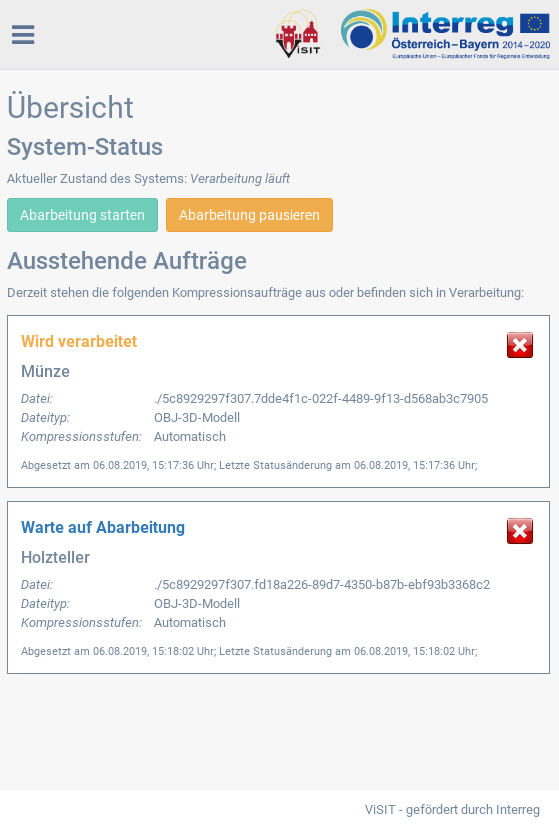
\includegraphics[width=0.55\textwidth]{Figures/schlenker/webui/overview.png}
\caption{Startseite, unter anderem mit einem Überblick über die laufenden und anstehenden Kompressions-Aufträge}
\label{schlenke:fig:webuiOverview}
\end{center}
\end{figure}

\subsubsection{Neuer Auftrag}

Über diese Seite, welche in \autoref{schlenke:fig:webuiDispatch} dargestellt ist, lassen sich manuelle Kompressionsaufträge absetzen, wobei dies normalerweise direkt beim Hochladen der Medien"=Datei von der Medien"=Datenbank übernommen wird. Soll dennoch manuell ein Auftrag abgesetzt werden, so müssen in dieser Ansicht die UID des Metadatums (Objekt-Identifikator, {\ttfamily objectID}) und die UID der digitalen Repräsentation (Medien-Identifikator, {\ttfamily mediaID}), deren Beziehung in Abbildung \autoref{fig:digrep} veranschaulicht wird, angegeben werden. Zusätzlich kann ein Unterverzeichnis angegeben werden (Basis-Pfad), in dem sich die zu komprimierende Datei befindet, wobei dieser Pfad stets in Bezug auf das in der Konfiguration angegebene {\ttfamily media\-File\-Root\-Directory} interpretiert wird. Außerdem muss ein Titel für die Datei angegeben werden, der beliebig gewählt werden kann und lediglich zur leichteren Identifizierung des Auftrags innerhalb des Kompressions-Systems dient. Des weiteren ist der Dateityp zu spezifizieren, wobei hier die Optionen PNG"=Bild, JPEG"=Bild und OBJ"=3D"=Modell zur Auswahl stehen. 

Für den Fall, dass ein 3D"=Modell komprimiert wird, können im darauffolgenden Abschnitt die gewünschten Kompressionsstufen festgelegt werden. Zum Einen steht die Option \glqq{}Automatisch\grqq{} zur Verfügung, die standardmäßig ausgewählt ist und alle in der Konfiguration spezifizierten Standard"=Kompressionsstufen umfasst. Weitere oder alternative Auflösungsstufen können durch die Wahl des Eintrags \glqq{}Feste Größe\grqq{} und die Angabe der gewünschten Vertex"=Anzahl hinzugefügt werden. Sämtliche derzeit angegebenen Auflösungsstufen werden aufgelistet und lassen sich mit Klick auf das Mülltonnen"=Symbol wieder entfernen.

\begin{figure}
\begin{center}
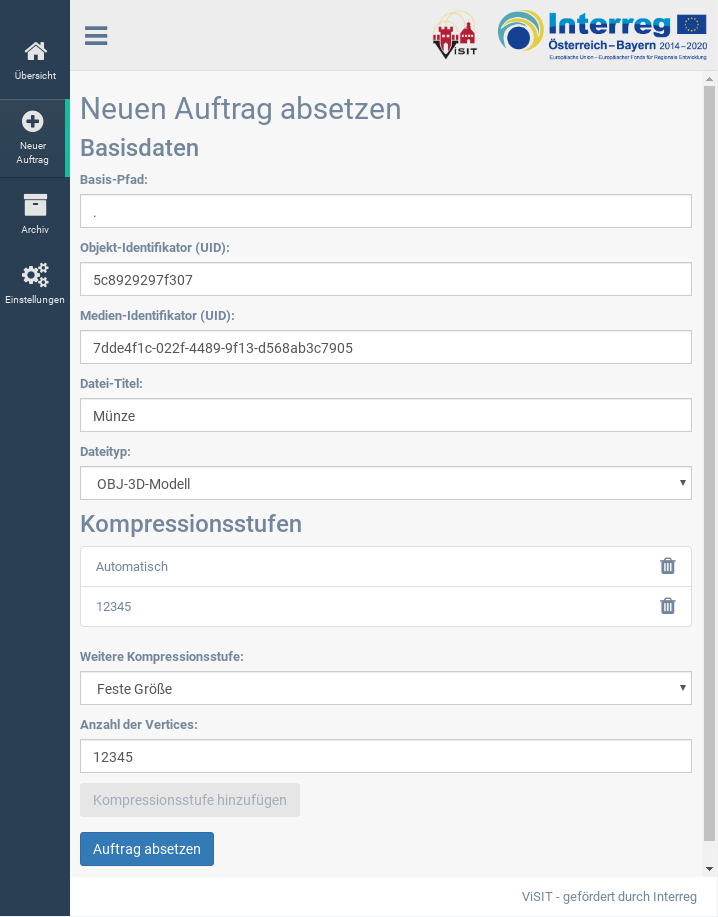
\includegraphics[width=0.55\textwidth]{Figures/schlenker/webui/dispatch2.png}
\caption{Ansicht zum Absetzen eines neuen Kompressions-Auftrags}
\label{schlenke:fig:webuiDispatch}
\end{center}
\end{figure}

\subsubsection{Archiv}

Über diese Ansicht lässt sich ein Überblick über die zuletzt abgearbeiteten Kompressions"=Aufträge erhalten, unabhängig davon, ob die Ausführung erfolgreich war oder fehlgeschlagen ist. Die Einträge werden nach der letzten Statusänderung absteigend sortiert, wobei die Anzahl der dargestellten Einträge in der Konfiguration festgelegt werden kann. Ein Beispiel für diese Ansicht ist in \autoref{schlenke:fig:webuiArchive} zu sehen.

\begin{figure}
\begin{center}
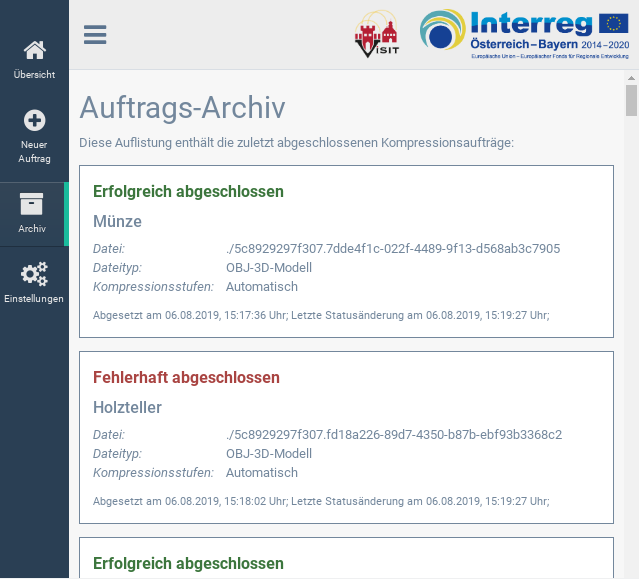
\includegraphics[width=0.55\textwidth]{Figures/schlenker/webui/archive.png}
\caption{Archiv-Ansicht mit einem Überblick über die ausgeführten Kompressions-Aufträge}
\label{schlenke:fig:webuiArchive}
\end{center}
\end{figure}

\subsubsection{Einstellungen}

Auf dieser Seite lassen sich die wichtigsten Konfigurations"=Optionen anpassen, wie in \autoref{schlenke:fig:webuiConfig} zu sehen ist. Alle Einstellungen, die auf dieser Seite nicht verfügbar sind, müssen manuell in der Konfigurationsdatei angepasst werden. Für Details zu den einzelnen Optionen wird auf Abschnitt \ref{schlenke:chp:configuration} verwiesen.

Die über die Web"=Oberfläche verfügbaren Konfigurationsmöglichkeiten werden im Folgenden aufgeführt, wobei auch die Entsprechung in der Konfigurationsdatei benannt wird. Sämtliche Angaben werden jedoch erst durch das Betätigen der Schaltfläche \glqq{}Einstellungen speichern\grqq{} am Ende der Seite zum Server übertragen und übernommen.
\begin{itemize}
\item \emph{Portnummer der API-Schnittstelle: } {\ttfamily apiPort}
\item \emph{Maximale Länge der Auftragsliste: } {\ttfamily queueMaxLength}
\item \emph{Abarbeitung automatisch beim Starten des Servers beginnen: } {\ttfamily autostart}
\item \emph{API"=Zugriffsberechtigte IP-Adressen: }{\ttfamily access\-White\-List\-Ips}. Die berechtigten IP-Adressen sind einzeln anzugeben und über die Schaltfläche \glqq{}IP-Adresse hinzufügen\grqq{} zu bestätigen. Durch einen Klick auf das Mülltonnen"=Symbol können Einträge wieder entfernt werden. Auch hier entspricht die Angabe eines Asterisks (\glqq{}$\ast$\grqq{}) einer Zugriffsgenehmigung für alle Hosts.
\item \emph{Standard-Kompressionsstufen für 3D-Modelle: }{\ttfamily defaultLevels}. Die Anzahl der Vertices der komprimierten Modelle, die bei der Kompression von 3D"=Modellen standardmäßig erstellt werden sollen, sind an dieser Stelle einzeln anzugeben und über die Schaltfläche \glqq{}Kompressionsstufe hinzufügen\grqq{} hinzuzufügen. Auch hier können einzelne Kompressionsstufen durch Betätigen des Mülleimer"=Symbols entfernt werden.
\item \emph{Kompression der Textur von 3D-Modellen: }{\ttfamily textureLimits}, {\ttfamily textureSizes}. Die Anzahl der Schwellwerte und demzufolge unterschiedlicher Textur-Auflösungen lässt sich über die beiden Schaltflächen \glqq{}Unterscheidung hinzufügen\grqq{} bzw. \glqq{}Unterscheidung entfernen\grqq{} kontrollieren. Die Texturgröße ist als Anzahl der Pixel pro Dimension zu verstehen.
\item \emph{Aktionen für die Kompression von Bildern: }{\ttfamily imageCompressionLevels}. Die für eingehende Bild"=Kompressions"=Aufträge zu erstellenden Auflösungsstufen sind hier aufgelistet, wobei sich einzelne Einträge durch das Betätigen des Mülleimer"=Symbols entfernen lassen. Weitere Kompressionsstufen lassen sich durch die Angabe eines beliebigen Titels, der nur aus Groß- oder Kleinbuchstaben, Ziffern und Binde- oder Unterstrichen bestehen darf, sowie der maximalen Breite und maximalen Höhe des komprimierten Bildes in Pixeln und anschließendes Betätigen der Schaltfläche \glqq{}Kompressionsstufe hinzufügen\grqq{} hinzufügen.
\end{itemize}

\begin{figure}
\centering
\subfloat{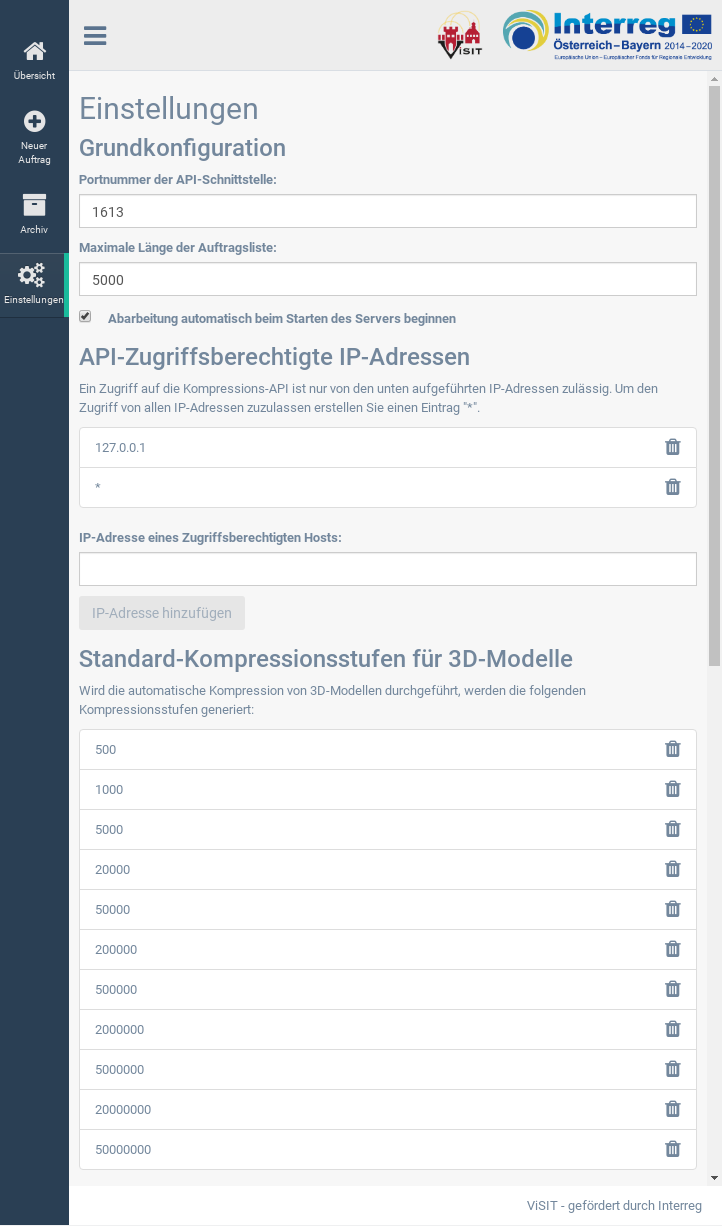
\includegraphics[width=0.45\textwidth]{Figures/schlenker/webui/config1.png}}
\qquad
\subfloat{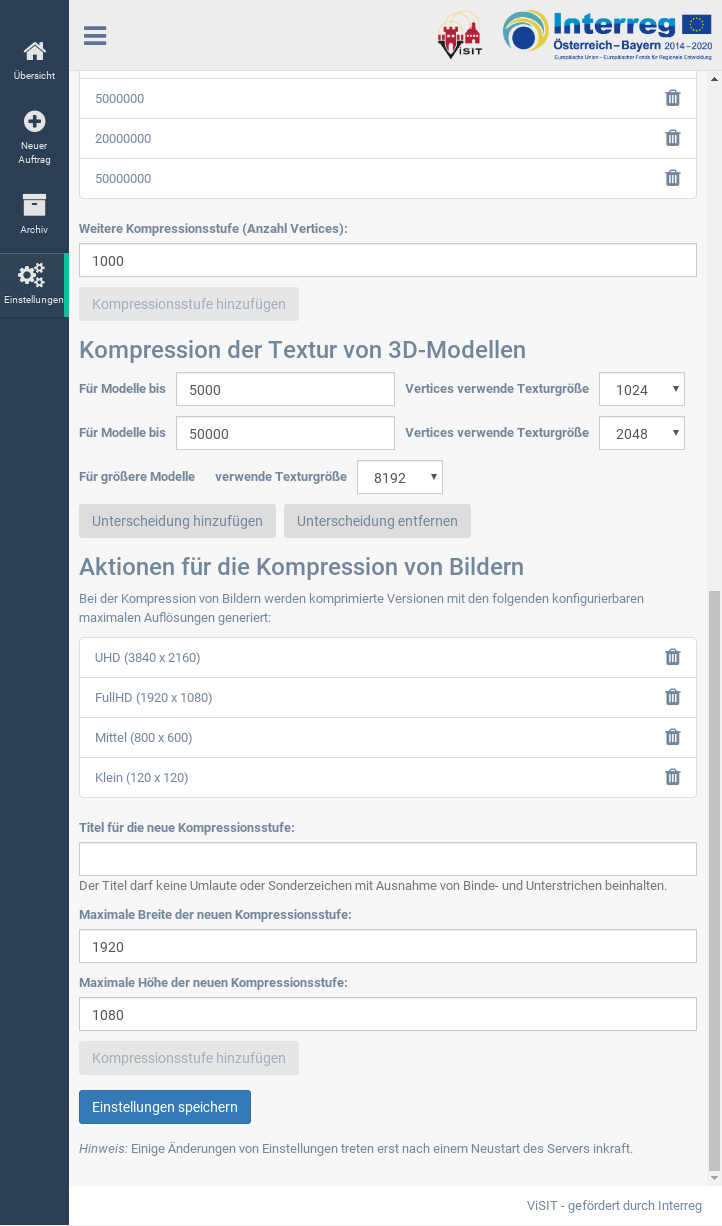
\includegraphics[width=0.45\textwidth]{Figures/schlenker/webui/config2.png}}
\caption{Einstellungsmöglichkeiten über die Web-Oberfläche}
\label{schlenke:fig:webuiConfig}
\end{figure}

\subsection{Zugriff über die API}
\label{schlenke:chp:api}

Sämtliche Funktionen der API stehen bei der standardmäßigen Konfiguration unter dem Basispfad \url{http://localhost:1613/api} zur Verfügung. Die API bietet unterschiedliche Module an, auf deren Funktionen in diesem Abschnitt eingegangen wird. POST"=Parameter sind stets als JSON"=Objekt zu übergeben, ebenso erfolgt die Antwort in Form eines JSON"=Objekts. 

\subsubsection{Aktuelle Kompressions-Aufträge}

Für Informationen zu den IDs, dem MIME"=Typen oder den Kompressions"=Stufen wird auf Abschnitt \ref{schlenke:chp:funktionsweise} verwiesen. Beim Absetzen wird jedem Kompressions"=Auftrag eine ID zugewiesen, welche zum Löschen des Auftrags angegeben werden muss. Der Status eines Auftrags kann einen der folgenden Werte annehmen:
\begin{itemize}
\item {\ttfamily ENQUEUED}: Der Auftrag wurde abgesetzt, mit der Abarbeitung wurde jedoch noch nicht begonnen.
\item {\ttfamily PROCESSING}: Der Auftrag wurde abgesetzt und befindet sich derzeit in Verarbeitung.
\item {\ttfamily ERROR}: Die Verarbeitung des Auftrags wurde fehlerhaft abgeschlossen.
\item {\ttfamily COMPLETED}: Die Verarbeitung des Auftrags wurde erfolgreich abgeschlossen.
\end{itemize}

\noindent\textbf{Funktion: }Absetzen eines Kompressions-Auftrags\\
\textbf{HTTP-Methode: } {\ttfamily POST} \\
\textbf{Pfad: } {\ttfamily /jobs/dispatch} \\
\textbf{POST-Paramter: }
\begin{lstlisting}[caption={POST-Parameter zum Absetzen eines Kompressions-Auftrags}]
{
		basePath : string, 	/* Unterverzeichnis, in welchem die Datei abgelegt ist, ansonsten "" */
		objectUid : string, /* objectTripleID (nicht objectTripleURL) der Medien-Datei */
		mediaUid : string, 	/* mediaTripleID (nicht mediaTripleURL) der zu komprimierenden Medien-Datei */
		title : string, 	  /* Beliebiger Titel zur Identifizierung des Kompressions-Auftrags */
		mimeType : string, 	/* MIME-Typ der zu komprimierenden Datei */
		levels : [string], 	/* Array mit den Bezeichnern aller gewuenschten Kompressions-Stufen */
}
\end{lstlisting}
\textbf{Antwort: }
\begin{lstlisting}[caption={Antwort auf das Absetzen eines Kompressions-Auftrags}]
{
		success : boolean,
		message : string
}
\end{lstlisting}

\noindent\textbf{Funktion: }Auflisten aller noch nicht abgeschlossenen Kompressions-Aufträge\\
\textbf{HTTP-Methode: } {\ttfamily GET} \\
\textbf{Pfad: } {\ttfamily /jobs/dispatch} \\
\textbf{Antwort: }
\begin{lstlisting}[caption={Antwort auf das Auflisten nicht abgeschlossener Kompressions-Aufträge}]
{
		success : boolean,
		message : string,
		items : [{
				job : {
						basePath : string, 	/* Unterverzeichnis, in welchem die Datei abgelegt ist, ansonsten "" */
						objectUid : string, /* objectTripleID (nicht objectTripleURL) der Medien-Datei */
						mediaUid : string, 	/* mediaTripleID (nicht mediaTripleURL) der Medien-Datei */
						title : string, 	  /* Beliebiger Titel zur Identifizierung des Kompressions-Auftrags */
						mimeType : string, 	/* MIME-Typ der zu komprimierenden Datei */
						levels : [string], 	/* Array mit den Bezeichnern aller gewuenschten Kompressions-Stufen */
				},
				receivedOn : timestamp,     /* UNIX-Timestamp, an dem der Auftrag abgesetzt wurde */
				id : int,                   /* Vom Kompressions-System vergebene ID fuer den Auftrag */
				state : string,             /* Aktueller Status des Auftrags, kann entweder ENQUEUED, PROCESSING, ERROR oder COMPLETED sein */
				lastStateChange : timestamp /* UNIX-Timestamp der letzten Statusaenderung des Auftrags */
		}]
}
\end{lstlisting}

\noindent\textbf{Funktion: }Löschen eines Kompressions-Auftrags\\
\textbf{HTTP-Methode: } {\ttfamily DELETE} \\
\textbf{Pfad: } {\ttfamily /jobs/cancel/\{ID\}}, mit \{ID\} der ID des Kompressions"=Auftrags \\
\textbf{Antwort: }
\begin{lstlisting}[caption={Antwort auf das Löschen eines Kompressions-Auftrags}]
{
		success : boolean,
		message : string
}
\end{lstlisting}

\subsubsection{Abgeschlossene Kompressions"=Aufträge}

\noindent\textbf{Funktion: }Auflisten der letzten abgeschlossenen Kompressions"=Aufträge\\
\textbf{HTTP-Methode: } {\ttfamily GET} \\
\textbf{Pfad: } {\ttfamily /archive/jobs/} \\
\textbf{Antwort: }
\begin{lstlisting}[caption={Antwort auf das Auflisten abgeschlossener Kompressions-Aufträge}]
{
		success : boolean,
		message : string,
		items : [{
				job : {
						basePath : string, 	/* Unterverzeichnis, in welchem die Datei abgelegt ist, ansonsten "" */
						objectUid : string, /* objectTripleID (nicht objectTripleURL) der Medien-Datei */
						mediaUid : string, 	/* mediaTripleID (nicht mediaTripleURL) der Medien-Datei */
						title : string, 	  /* Beliebiger Titel zur Identifizierung des Kompressions-Auftrags */
						mimeType : string, 	/* MIME-Typ der zu komprimierenden Datei */
						levels : [string], 	/* Array mit den Bezeichnern aller gewuenschten Kompressions-Stufen */
				},
				receivedOn : timestamp,     /* UNIX-Timestamp, an dem der Auftrag abgesetzt wurde */
				id : integer,               /* Vom Kompressions-System vergebene ID fuer den Auftrag */
				state : string,             /* Aktueller Status des Auftrags, kann entweder ENQUEUED, PROCESSING, ERROR oder COMPLETED sein */
				lastStateChange : timestamp /* UNIX-Timestamp der letzten Statusaenderung des Auftrags */
		}]
		
}
\end{lstlisting}

\subsubsection{Status des Kompressions-Systems}

Der Zustand des Kompressions"=Systems kann einen der folgenden Werte annehmen:
\begin{itemize}
\item {\ttfamily STARTUP:} Das System wird hochgefahren, mit der Abarbeitung von Kompressions"=Aufträgen wurde noch nicht begonnen.
\item {\ttfamily RUNNING:} Das System ist hochgefahren und bearbeitet Kompressions"=Aufträge oder ist bereit dazu.
\item {\ttfamily PAUSED:} Das System ist hochgefahren, die Abarbeitung von Kompressions"=Aufträgen wurde jedoch pausiert.
\item {\ttfamily SHUTTINGDOWN:} Das System wird heruntergefahren, weshalb das Absetzen weiterer Aufträge nicht möglich ist. Jedoch werden noch Kompressions"=Aufträge verarbeitet.
\item {\ttfamily SHUTDOWN:} Das System wurde heruntergefahren. Es können keine weiteren Aufträge abgesetzt oder verarbeitet werden.
\end{itemize}

Zum Setzen des Zustands des Kompressions"=Systems kann einer der folgenden Werte verwendet werden:
\begin{itemize}
\item {\ttfamily RUN:} Setze den Zustand auf {\ttfamily RUNNING} und beginne mit der Bearbeitung von Kompressions"=Aufträgen. Dieses Kommando ist nur in den Zuständen {\ttfamily PAUSED} oder {\ttfamily STARTUP} zulässig.
\item {\ttfamily PAUSE:} Setze den Zustand auf {\ttfamily PAUSED} und pausiere damit die Abarbeitung der Kompressions"=Aufträge nach dem Abschließen des aktuellen Auftrags. Dieses Kommando ist nur im Zustand {\ttfamily RUNNING} zulässig.
\item {\ttfamily SHUTDOWN\_PROCESS\_QUEUE:} Setze den Zustand auf {\ttfamily SHUTTINGDOWN}, verarbeite aber vor dem Herunterfahren die gesamte Auftragsliste. Dieses Kommando ist nur im Zustand {\ttfamily STARTUP}, {\ttfamily RUNNING} oder {\ttfamily PAUSED} zulässig.
\item {\ttfamily SHUTDOWN\_IMMEDIATELY:} Setze den Zustand auf {\ttfamily SHUTTINGDOWN}, schließe aber vor dem Herunterfahren den sich aktuell in Verarbeitung befindlichen Auftrag ab.  Dieses Kommando ist nur im Zustand {\ttfamily STARTUP}, {\ttfamily RUNNING} oder {\ttfamily PAUSED} zulässig.
\item {\ttfamily KILL}: Setze den Zustand auf {\ttfamily SHUTDOWN}, fahre das System herunter ohne Rücksicht auf ausstehende oder sich in Verarbeitung befindliche Kompressions"=Aufträge.
\end{itemize}

\noindent\textbf{Funktion: }Abrufen des Systemzustands \\
\textbf{HTTP-Methode: } {\ttfamily GET} \\
\textbf{Pfad: } {\ttfamily /control/state} \\
\textbf{Antwort: }
\begin{lstlisting}[caption={Antwort auf das Abrufen des Systemzustands}]
{
		success : boolean,
		message : string,
		state : string		/* {STARTUP | RUNNING | PAUSED | SHUTTINGDOWN | SHUTDOWN} */
}
\end{lstlisting}

\noindent\textbf{Funktion: }Setzen des Systemzustands \\
\textbf{HTTP-Methode: } {\ttfamily PUT} \\
\textbf{Pfad: } {\ttfamily /control/state} \\
\textbf{POST-Paramter: }
\begin{lstlisting}[caption={POST-Parameter zum Setzen des Systemzustands}]
{
		state : string   	/* {RUN | PAUSE | SHUTDOWN_PROCESS_QUEUE | SHUTDOWN_IMMEDIATELY | KILL} */
}
\end{lstlisting}
\textbf{Antwort: }
\begin{lstlisting}[caption={Antwort auf das Setzen des Systemzustands}]
{
		success : boolean,
		message : string
}
\end{lstlisting}

\subsubsection{Konfiguration des Kompressions"=Systems}

Für Details zu den einzelnen Konfigurationsoptionen wird auf Abschnitt \ref{schlenke:chp:configuration} verwiesen.

\noindent\textbf{Funktion: }Abrufen der Systemkonfiguration \\
\textbf{HTTP-Methode: } {\ttfamily GET} \\
\textbf{Pfad: } {\ttfamily /settings/config} \\
\textbf{Antwort: }
\begin{lstlisting}[caption={Antwort auf das Abrufen der Systemkonfiguration}]
{
		success : boolean,
		message : string,
		config : {
				apiPort : integer,
				apiAccessWhitelist : [string],
				autostart : boolean,
				queueMaxLength : integer,
				defaultLevels : [string],
				textureLevelLimits : [integer],
				textureLevelSizes : [integer]
				imageCompressionLevels : [{
						maxWidth : integer,
						maxHeight : integer,
						title : string
				}]
		}
		
}
\end{lstlisting}

\noindent\textbf{Funktion: }Setzen der Systemkonfiguration \\
\textbf{HTTP-Methode: } {\ttfamily PUT} \\
\textbf{Pfad: } {\ttfamily /settings/config} \\
\textbf{POST-Paramter: } 
\begin{lstlisting}[caption={POST-Parameter zum Setzen der Systemkonfiguration}]
{
		apiPort : integer,
		apiAccessWhitelist : [string],
		autostart : boolean,
		queueMaxLength : integer,
		defaultLevels : [string],
		textureLevelLimits : [integer],
		textureLevelSizes : [integer]
		imageCompressionLevels : [{
				maxWidth : integer,
				maxHeight : integer,
				title : string
		}]
}
\end{lstlisting}
\textbf{Antwort: }
\begin{lstlisting}[caption={Antwort auf das Setzen der Systemkonfiguration}]
{
		success : boolean,
		message : string
}
\end{lstlisting}






\section{ViSIT Metadaten und die Semantische Datenbank}\label{sec:semantics}

Brainstorm, things to write about:

\begin{itemize}
	\item theoretischer background: rdf daten, CIDOC, Vismo
	\item datenbank: infrastruktur (hosting, allgemeiner zugriff von aussen), drupal, wisski (allgemein), grundfunktionalität
	\item wisski: rdf daten, pfade, konfiguration
	\item REST API: allgemeine beschreibung
	\item zusatzfeatures: copy and paste, excel import
\end{itemize}

\subsection{Theoretische Grundlagen für die Semantische Datenbank}\label{sec:theoreticalBackground}

Dieses Unterkapitel gibt Einblicke in Teilbereiche des Semantic Webs, um eine theoretische Grundlage für die folgenden technischen Entwicklungen zu geben. Nachdem diese erläutert wurden, wird ebenfalls auf eine spezielle Ausprägung eines Metadatenmodells eingegangen, welches die Struktur für die im ViSIT Projekt verwendeten Metadaten vorgibt: das ViSIT Model \textbf{VisMo}.

Die hier angeführten Ausführungen beschränken sich jedoch nur auf jeweilige Grundlagen der Themenkomplexe, welche an manchen Stellen um weiterführende Informationen erweitert werden, wenn dies für den weiteren Verlauf von Nöten ist. Dennoch, falls angestrebt, verweisen wir für ein tieferes Verständnis auf weitere Fachliteratur, wie z.B. \cite{Hitzler-SemanticWeb-2007}.

\paragraph{Semantic Web und RDF Daten}

Das Semantic Web ist eine Art Erweiterung zum eigentlichen World Wide Web, wie wir es aktuell kennen. Dieses ist primär für Menschen ausgelegt, die durch Homepages browsen und dabei entsprechende Informationen durch betrachten und lesen der Homepages erlangen. Diese Informationen sind dadurch jedoch nur für Menschen vorhanden, Maschinen oder Computer können auf die Informationen nicht zugreifen, um mit den entsprechenden Daten arbeiten zu können. Genau hier setzt das Semantic Web an, welches Standardisierungen, Regeln und Prozesse vorgibt, um Homepages und Applikationen so anzupassen, dass eben genau eine (semi-) automatische Informationsverarbeitung für Maschinen möglich wird.
 
Eine dieser Standardisierungen ist das Resource Description Framework \textbf{RDF} \cite{Manola-RDFPrimer1.0-2004}, welches der de-facto Standart im Semantic Web ist, um Metadaten zu beschreiben. Daten in RDF werden als Graph modelliert und persistiert, welcher aus Knoten und Kanten besteht. Dabei entsteht eine Wissensbasis gefüllt an Informationen. Die Knoten sind hierbei die \q{Akteure}, also diejenigen Entitäten, Sachen, Objekte, Dinge etc., ausgehend vom jeweiligen Anwendungsfall, auf die sich die im Graphen enthaltenen Informationen beziehen (diese Dinge werden im Folgenden weiterhin als \q{Metadatenentität} bezeichnet). Die Kanten im Graphen beschreiben Beziehungen zwischen den gegebenen Knoten und Eigenschaften der Knoten. Weiterhin sind die Knoten und Kanten durch das Grundprinzip eines \textbf{Statements} verbunden, welches eine Kapselung einer elementaren Aussage darstellt. Das Statement ist, ähnlich dem deutschen Satzbau, immer bestehend aus drei Teilen:

\begin{description}
	\item[Subjekt] Die Metadatenentität repräsentiert als ein Knoten im Graphen, von der die Aussage - und damit das Prädikat - des Statements ausgeht.
	\item[Prädikat] Die Semantik oder die Bedeutung der Aussage.
	\item[Objekt] Zweierlei Konzepte können das Objekt des Statements bilden: ein weiterer Knoten im Graphen, um das Ziel der Aussage und damit des Prädikats, um eine Relation zwischen zwei Metadatenentitäten/Knoten darzustellen, oder ein fester Wert, um eine Eigenschaft einer Metadatenentitäten/eines Knotens zu charakterisieren.
\end{description}

Zur Verständlichkeit für die Thematik der Aussagen und Statements im Semantic Web Kontext, soll hier ein kurzes, erfundenes Beispiel erläutert werden. Folgende Aussagen bilden die Wissensbasis:

\begin{itemize}
	\item Peter ist vom Beruf Baumeister.
	\item Peter ist 40 Jahre alt.
	\item Peter war am Bau des Steinschlosses beteiligt.
	\item Das Steinschloss besteht aus Stein.
	\item Das Steinschloss ist 10 Jahre alt.
\end{itemize}

Wie oben beschrieben, bestehen die Aussagen jeweils aus Subjekt, Prädikat und Objekt. Als Subjekte agieren die beiden Metadatenentitäten \q{Peter} und das \q{Steinschloss}, während die Objekte der Aussagen der Beruf \q{Baumeister}, das Material \q{Stein}, zwei \q{Altersangaben}, sowie das \q{Steinschloss} selbst sind. Semantisch sind die Subjekte und Objekte über die Beziehungen bzw. Eigenschaften einer \q{Berufszuordnung}, zwei \q{Alterszuordnungen}, einer \q{Materialzuweisung} sowie der \q{Erbauung} eines Objekts verbunden.

Diese Aussagen können nun in einen Graphen zusammengefasst werden, dessen high-level Illustration in \autoref{fig:statements} zu sehen ist.

\begin{figure}[htb]
    \centering
    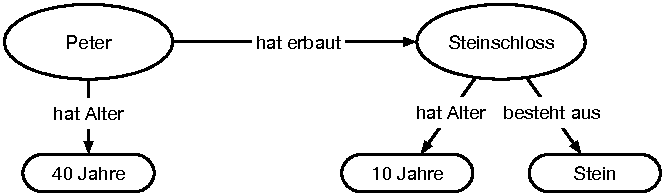
\includegraphics[width=\textwidth]{Figures/berndl/statements}
    \caption{\label{fig:statements} Informationen aus obigen Aussagen, kombiniert als Graph.}
\end{figure}

\paragraph{Linked Open Data Gedanke}

Ein weiterer Eckpfeiler des Semantic Web ist ein weiteres Konzept, das unter dem Namen \textbf{Linked Open Data - LOD} bekannt ist. Oft wird dieser Name ebenfalls für das Semantic Web selbst benutzt, die punktgenauen Definitionen überschneiden und ergänzen sich.

Einfach übersetzt zielt LOD auf öffentlich zugängliche Daten ab, die untereinander vernetzt und verlinkt sind. Somit soll es möglich sein, verteilte Datenbanken mit ihren eigenen entsprechenden Wissensbasen, miteinander zu verbinden, um so jedem Beteiligten mehr Informationen zur Verfügung zu stellen, da durch die Verlinkung einzelner Graphen ein großer Gesamtgraph entsteht. Auf diese Weise macht es Sinn, dass jede Wissensbasis ihren eigenen spezialisierten Kontext besitzt. Sollte eine Wissensbasis weitere Informationen aus einem anderen Kontext benötigen, müssen diese Daten nicht auf eigene Hand erforscht und aufbereitet werden, da eine LOD Verbindung zu einer anderen Wissensbasis hergestellt werden kann. Zur weiteren Veranschaulichung dieser Thematik und dessen Vorteile, zeigt der folgende Paragraph zwei Anwendungsfälle im geschichtswissenschaftlichen Kontext.

\paragraph{Zwei Anwendungsfälle für RDF im Geschichtswissenschaftlichen Kontext}

Ein erster Anwendungsfall, von dem geisteswissenschaftliche Wissensbasen profitieren können, ist oben bereits kurz angedeutet worden: das Verbinden einer eigenen Wissensbasis mit externen, bereits bestehenden Wissensbasen. Das Erforschen und Erkunden von Wissen benötigt generell in jeglichem Kontext sehr viel Zeit und ebenfalls Pflege der Daten. Daher kommt diesem Anwendungsfall der LOD Gedanke entgegen, da bereits erstellte Wissensbasen und deren Datenbanken öffentlich zugänglich sind.

Gerade generelle Themen oder Kontexte wie Personen, Städte oder Orte werden in vielen geschichtswissenschaftlichen Projekten benötigt, und gerade diese sind in öffentlichen Datenbanken zugänglich. Daher ist es für diese Anwendungsfälle sinnvoll, den eigens entwickelten Anwendungsfall an diese Datenbanken zu knüpfen. Dadurch wird der eigene Zeitaufwand erheblich reduziert und die angebundenen Daten genießen in der Regel außerdem einen hohen Standard, da bereits viele potenzielle Reviews von anderen Nutzern bestehen.

Ein zweiter großer Vorteil davon, geschichtswissenschaftliche Daten in Form von Metadaten und RDF zu persistieren, ist das mögliche Erschließen von vorher nicht bekannten oder erforschten Zusammenhänge der persistierten Objekte. Dazu folgendes (frei erfundenes) Beispiel: Ausgehend von der eigenen Wissensbasis, die die Daten aus \autoref{fig:statements} enthält, sollen nun zwei weitere Wissensbasen angekoppelt werden, welche auf der einen Seite weitere Informationen über Personen und vor allem deren familiärer Beziehungen beinhaltet, und auf der anderen Seite eine Wissensbasis, die mehr Informationen über Gebäude und deren Geschichte beinhaltet. Dies ist in \autoref{fig:extendedStatements} visualisiert.

\begin{figure}[htb]
    \centering
    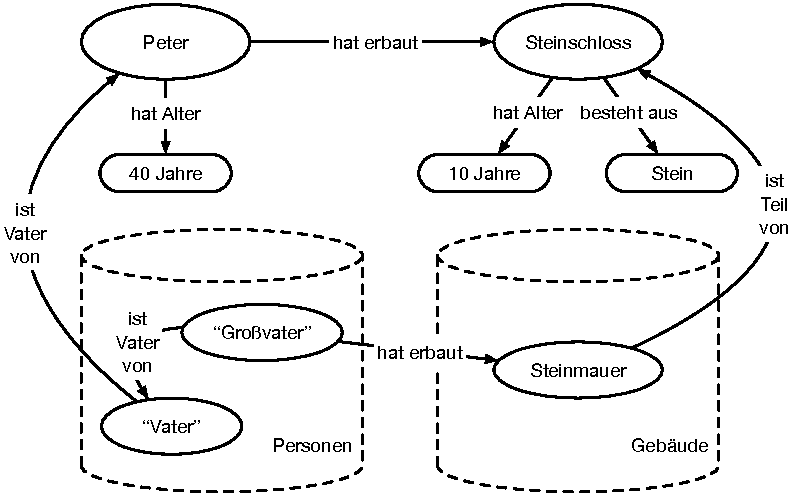
\includegraphics[width=\textwidth]{Figures/berndl/extendedStatements}
    \caption{\label{fig:extendedStatements} Grundlegende eigene Wissensbasis (oben), erweitert um zwei externe Wissensbasen (unten).}
\end{figure}

In dem Beispiel beinhaltet die eigene Wissensbasis Informationen über \q{Peter} und das \q{Steinschloss}. Durch die beiden hinzugenommenen Wissensbasen wird Peter aus dem Anwendungsbeispiel mit seinem \q{Vater}, und dieser wiederum mit seinem \q{Großvater} verbunden (die Namen sind hier zur Einfachheit ersetzt). Zudem wird die \q{Steinmauer} als ein Teil des Steinschlosses deklariert. Die beiden neuen Wissensbasen enthalten darüber hinaus bereits implizit eine eigene Verbindung, die semantisch besagt, dass der \q{Großvater} am Bau der Steinmauer beteiligt ist.

Dadurch erweitern die beiden externen Wissensbasen die eigenen Informationen durch die neu erstellten Relationen. Darüber hinaus jedoch lässt sich so ebenfalls eine neue Erkenntnis in den Daten schliessen: sowohl \q{Peter} als auch dessen \q{Großvater} sind direkt oder indirekt am Bau des \q{Steinschlosses} beteiligt.

\paragraph{Das Contextual Reference Model - CIDOC CRM}

Bisher war die technische Beschreibung der semantischen Daten im ViSIT Kontext aus Gründen der Einfachheit sehr flach gehalten. Gemäß den Semantic Web Standards basieren die Metadaten jedoch auf einem Datenmodell, um die Anforderungen des Semantic Webs zu genügen und ebenfalls technische Verabeitbarkeit zu gewährleisten.

In ViSIT ist die Wahl hierbei auf das \textbf{Contextual Reference Model CIDOC CRM} \cite{CIDOC-Doerr-2003} gefallen, da dies eine der bekanntesten und vorherrschendsten Ontologien im Bereich des kulturellen Erbes ist. Diese Ontologie wird als Basis benutzt, die im folgenden Paragraphen erweitert für den ViSIT Kontext beschrieben wird. Der größte Vorteil dieser Ontologie ist, dass sie sich nicht auf einen speziellen Bereich des kulturellem Erbes fokussiert ist, sondern auf generische Weise komplexe Zusammenhänge und verschiedene Themengebiete abbildet. Zudem solle es möglich sein, andere Ontologien oder Modelle aus dem selben Bereich in diese Ontologie zu überführen, um eine gemeinsam verständliche Wissensbasis zu kreieren.

Das CIDOC CRM wird seit mittlerweile über 10 Jahren von der CIDOC Documentation Standards Working Group\footnote{\url{http://network.icom.museum/cidoc/working-groups/overview/}} und der CIDOC CRM SIG\footnote{\url{http://network.icom.museum/cidoc/working-groups/crm-special-interest-group/}} entwickelt, welche beide Arbeitsgruppen von CIDOC\footnote{\url{http://network.icom.museum/cidoc/}} sind. Das CIDOC CRM ist 2000 als \q{Working Draft} bei der ISO/TC46/SC4\footnote{\url{https://www.iso.org/committee/48798.html}} akzeptiert worden, welcher 2006 schliesslich auch als offizieller Standard \cite{CIDOCCRM-iso21127:2006} akzeptiert wurde, und 2014 in eine überarbeitete Version \cite{CIDOCCRM-iso21127:2014} überführt wurde.

In der aktuellen Hauptversion 6.2\footnote{\url{http://www.cidoc-crm.org/Version/version-6.2}}, die im Mai 2015 veröffentlicht wurde, enthält die Ontologie 89 RDF Klassen und 149 einzigartige Relationen und Eigenschaften, die sich in einer mehrfach ineinander- sowie auseinander verzweigenden Struktur einordnen. Laufend werden ebenfalls Nebenversionen veröffentlicht - die aktuellste Versionsnummer lautet 6.2.3\footnote{\url{http://www.cidoc-crm.org/Version/version-6.2.3}}.

\paragraph{Das ViSIT Model - VisMo}

Aufbauend auf dem CIDOC CRM wurde eine Ontologie entwickelt, die den kompletten Anwendungsfall des ViSIT Projekt abbilden kann: das \textbf{ViSIT Model VisMo}. Der Fokus liegt dabei auf der Darstellung von Architektur-Objekten und Ausstellungsobjekten, die mit Personen oder Gruppen von Personen, Orten sowie zeitlichen Events in Verbindung gesetzt werden, um eine Wissensbasis zu kreieren.

Diesbezüglich sind die Hauptentitäten, die in der \visit Datenbank angelegt werden können, die folgenden:

\begin{description}
	\item[Ereignis (Activity):] Diese Entität umfasst alle vergangenen und zukünftigen Vorgänge und Geschehnisse in kulturellen, sozialen und physischen Systemen, analog zum \texttt{\q{E5\_Event}}\footnote{\url{http://www.cidoc-crm.org/Entity/E5-Event/Version-6.2}} des CIDOC CRM.
	\item[Bauwerk (Architecture):] Diese Entität bezeichnet alle Arten von Bauten, die wie die Objekte als Informationsträger (vgl. \texttt{\q{E84\_\-In\-for\-ma\-tion\_Car\-rier}}\footnote{\url{http://www.cidoc-crm.org/Entity/E84-Information-Carrier/Version-6.2}} des CIDOC CRM) betrachtet werden.
	\item[Gruppe (Group):] Diese Entität bezeichnet mehrere Personen, die sich zu einer Gruppierung zusammengeschlossen haben und durch eine gleiche oder ähnliche Tätigkeit miteinander verbunden sind (vgl. \texttt{\q{E74\_\-Group}}\footnote{\url{http://www.cidoc-crm.org/Entity/E74-Group/Version-6.2}} des CIDOC CRM).
	\item[Institution (Institution):] Diese Entität bezeichnet hier alle Arten von organisierten Einrichtungen, die keine natürlichen Personen oder Personengruppen sind, z.B. Museen, Archive, Bibliotheken, Universitäten usw.
	\item[Objekt (Object):] Diese Entität bezeichnet alle Arten von Ausstellungsobjekten aus den Sammlungen von musealen oder museumsähnlichen Institutionen, Archiven etc. , die wie Bauwerke als Informationsträger betrachtet werden (vgl. \texttt{\q{E84\_\-In\-for\-ma\-tion\_Car\-rier}}\footnote{\url{http://www.cidoc-crm.org/Entity/E84-Information-Carrier/Version-6.2}} des CIDOC CRM).
	\item[Person (Person):] Diese Entität bezeichnet analog zur Definition im CIDOC CRM der \texttt{\q{E21\_Person}}\footnote{\url{http://www.cidoc-crm.org/Entity/E21-Person/Version-6.2)}} alle natürlichen Personen, die leben oder bereits verstorben sind sowie Personen, von denen angenommen wird, dass sie lebten. Dazu zählen historische Persönlichkeiten als auch Personen aus Legenden, Mythen und Sagen.
	\item[Ort (Place):] Diese Entität bezeichnet hier ausschließlich über Koordinaten lokalisierbare verschwundene und bestehende Dörfer und Städte.
	\item[Literatur (Reference):] Diese Entität bezeichnet alle Arten von niedergeschriebenen und veröffentlichen Texten.
\end{description}

Dabei erfüllt VisMo genau den Zweck, den sich das CIDOC CRM als Ziel gesetzt hat: als eine semantische \q{Erweiterung} des CIDOC CRM ist der Inhalt, der für VisMo produziert wird, direkt zum größten Teil verständlich und Leser oder Benutzer des Modells können dies intuitiver, auf der Basis der Beschreibungen des CIDOC CRM, verstehen, lesen und benutzen. Dies ist dadurch begründet, dass alle Klassen und viele der Relationen und Eigenschaften durch Vererbung speziellere Konzepte der CIDOC CRM Klassen und Relationen/Eigenschaften sind. Nur einzelne Teile des VisMo sind speziell für die Ontologie hinzugefügt worden, immer wenn kein Konzept aus dem CIDOC CRM passend für eine Vererbung war. \autoref{fig:modelworkflow} visualisiert den Entwicklungsprozess hinter VisMo.

\begin{figure}[htb]
    \centering
    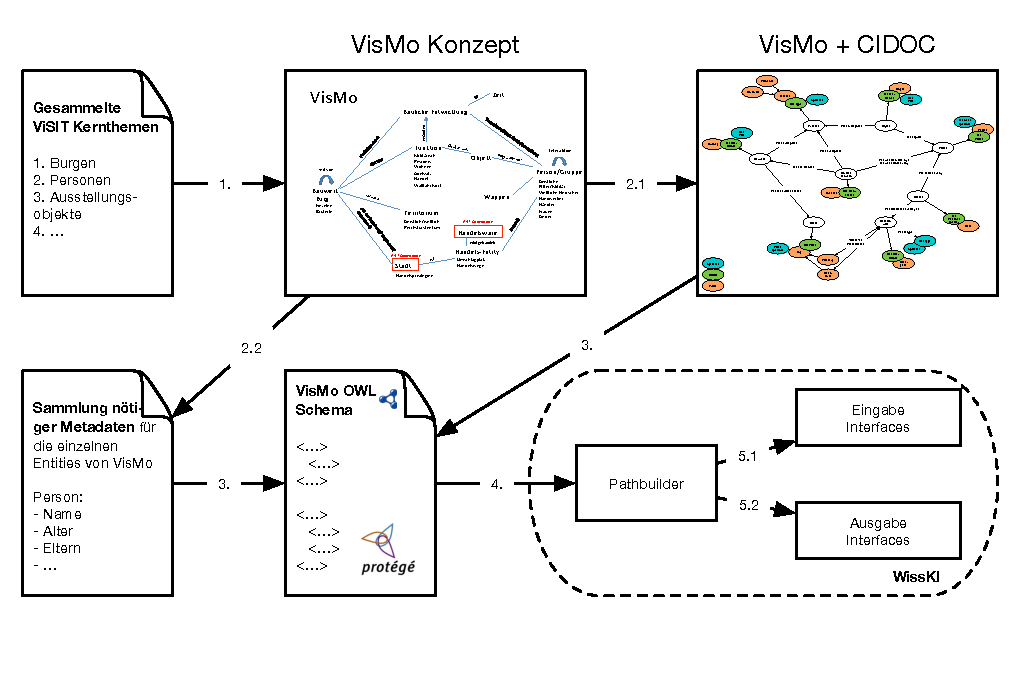
\includegraphics[width=\textwidth]{Figures/berndl/modelworkflow}
    \caption{\label{fig:modelworkflow} Arbeitsprozess hinter der Entwicklung des ViSIT Modells.}
\end{figure}

Der erste Schritt bestand dabei in der Sammlung der Kernthemen, die in ViSIT behandelt werden. Aus diesen konnte dann im nächsten Schritt ein grobes Konzept entwickelt werden, welches anschließend in RDF übertragen werden konnte. Wie oben beschrieben, wurde hierbei von CIDOC CRM Grundklassen und Relationen bzw. Eigenschaften ausgegangen, welche dann für den ViSIT Kontext erweitert und angepasst wurden. Als nächstes konnten dann die erstmals groben Konzepte und Entitäten mit benötigten Metadaten bzw. dessen Anforderungen erweitert werden. Die Ergebnisse der vorherigen Schritte konnten dann letztendlich in dem Ontologie-Editor \textbf{protegé}\footnote{\url{https://protege.stanford.edu/}} zusammengeführt werden, um eine RDF/OWL Ontologie zu erstellen. Diese ist in ihrer letzten offiziellen Version in \autoref{lst:vismo} im Appendix zu sehen.

Ebenfalls ist in \autoref{fig:modelworkflow} visualisiert, wie und an welcher Stelle die VisMo Ontologie technisch zum Einsatz kommt: sie dient als Input für das sogenannte \wisski Modul, um aus der Ontologie Ein- sowie Ausgabemasken zu generieren, welche letztendlich vom Endnutzer des ViSIT Systems benutzt werden, um einerseits Daten in die semantische Datenbank einzutragen und diese dann auch wieder auszulesen und anzuzeigen. Der große Vorteil an diesem Prozess ist, dass der Endnutzer keinerlei Wissen über das Semantic Web und seine Technologien benötigt, da der oben beschriebene Prozess davon abstrahiert. Damit schreiben und lesen die Endnutzer im Endeffekt RDF, ohne davon zu wissen. Technische Details zu diesem Prozess sowie \wisski werden in folgenden Unterkapiteln gegeben.

\subsection{Technische Details zur Semantischen Datenbank}\label{sec:technicalBackground}

Nachdem \autoref{sec:theoreticalBackground} die theoretische Grundlage für die Semantische Datenbank beschrieben hat, fokussiert sich dieses Unterkapitel auf die technischen Aspekte der Datenbank. Dazu zählt in erster Linie die \textbf{allgemeine Infrastruktur}, das \textbf{Hosting} an der Universität Passau, der \textbf{allgemeine Zugriff auf die Datenbank}, getroffene Entscheidungen bezüglich \textbf{Security und Zertifizierungen}, sowie die anschließende Beschreibung einzelner Komponenten: dem \textbf{CMS Drupal}, dessen Modul \textbf{\wisski}, die \textbf{ViSIT REST API}, der unterliegende RDF Triplestore \textbf{RDF4J} und dessen generelle Funktionalität.

Für die semantische Datenbank wurde zur Projektlaufzeit aus Testzwecken ebenfalls eine Testinstanz ins Leben gerufen, welche eine komplette Spiegelung des damals aktuellen Systems ist. Die beiden Haupt-URLs der Server sind:

\begin{itemize}
	\item \texttt{https://database.visit.uni-passau.de/}
	\item \texttt{https://database-test.visit.uni-passau.de/}
\end{itemize}

Von diesen beiden Base-URLs ausgehend sind die weiteren Komponenten über folgende URL-Zusätze zu erreichen:

\begin{itemize}
	\item \textbf{Drupal/\wisski:} Base URL + \texttt{/drupal}
	\item \textbf{RDF4J:} Base URL + \texttt{/rdf4j-workbench}
	\item \textbf{Tomcat:} Base URL (ohne Zusatz)
	\item \textbf{ViSIT REST API:} Base URL + \texttt{/metadb-rest-api}
	\item \textbf{API Beschreibung:} Base URL + \texttt{/metadb-test-api/swagger-ui.html}
\end{itemize}

\paragraph{Infrastruktur}

Die Semantische Datenbank des ViSIT Projekts ist auf einem virtuellen Server an der Universität Passau installiert. Die allgemeine Infrastruktur ist in \autoref{fig:infrastructure} zu sehen.

\begin{figure}[htb]
    \centering
    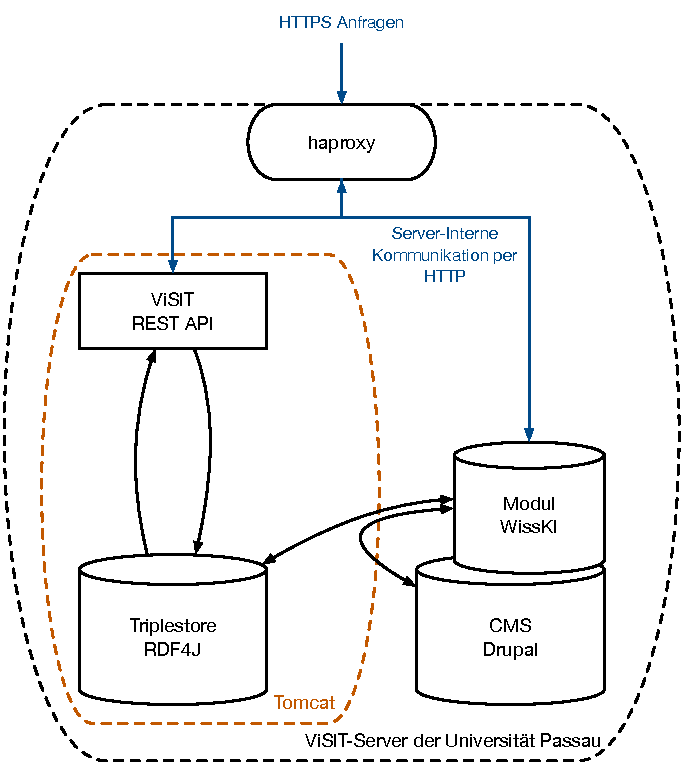
\includegraphics[width=\textwidth]{Figures/berndl/infrastructure}
    \caption{\label{fig:infrastructure} Technische Infrastruktur der Semantischen Datenbank des ViSIT Projekts.}
\end{figure}

Dessen Hauptkomponenten mit Beschreibung oder Verweis auf das ausführliche Unterkapitel sind die folgenden:

\begin{description}
	\item[haproxy] Dem virtuellen Server für die ViSIT Infrastruktur ist ein \textbf{haproxy}\footnote{\url{http://www.haproxy.org/}} vorgeschaltet. Dieser ist dafür da, die per HTTPS verschlüsselten Anfragen von aussen an den Server entgegen zu nehmen, und intern an die richtigen Komponenten weiterzuleiten. Prinzipiell kann dieser haproxy ebenfalls Anfragen per HTTP entgegen nehmen, leitet diese dann aber automatisch auf den Port für HTTPS weiter. Damit ist sicher gestellt, dass nach aussen nur verschlüsselte Daten versandt werden. Dem haproxy sind für die benötigte Funktionalität zwei backends bekannt: eines für den Tomcat (ViSIT REST API und Triplestore RDF4J) und eines für Drupal bzw. \wisski (welche hintergründig auf einem Apache laufen). Die Verschlüsselung ist durch ein SSL Zertifikat der Universität gewährleistet. Die Konfiguration zum haproxy is am Server zu finden unter \texttt{/etc/haproxy}.
	\item[Tomcat] Zur Installation weiterer Komponenten am Server, ist ein \textbf{Apache Tomcat}\footnote{\url{http://tomcat.apache.org/}} in der Version 8.5.24 installiert. Am Server ist dieser zu finden unter \texttt{/opt/tomcat8/apache-tomcat-8.5.24}.
	\item[ViSIT REST API] Diese API wurde eigens für ViSIT entwickelt, um eine Abstraktionsschicht für die unterliegenden Metadaten zu bieten. Während \wisski diese Abstraktion für die wissenschaftlichen Benutzer der Metadaten bildet, ist die API für die technische Anbindung der restlichen Komponenten des ViSIT Projekts zuständig. Die API bietet in erster Linie die Möglichkeit, die RDF Metadaten aus dem Triplestore zu lesen. Zurückgegeben wird das Ergebnis im JSON Format, um eine möglichst breite Verständnis und damit direkte Verwendbarkeit zu gewährleisten. Der zweite große Teil behandelt das Schreiben, Auslesen und Updaten der sogenannten technischen Metadaten: Metadaten, die Informationen zu einem Medien-Objekt im ViSIT Kontext geben. Die REST API ist als eigenständiges Java-Projekt implementiert, welches auf dem ViSIT Server bzw. in dessen Tomcat Installation deployed wird. Eine ausführliche Beschreibung wird in \autoref{sec:rest} gegeben.
	\item[Triplestore RDF4J] Der Triplestore ist für die Persistierung der RDF Daten zuständig. Im ViSIT Kontext ist die Wahl hierfür auf die \textbf{RDF4J}\footnote{\url{http://rdf4j.org/}} Datenbank gefallen, dieser ist jedoch durch jeglichen gleichwertigen Triplestore ersetzbar. Wie bei der REST API beschrieben, wird im ViSIT Kontext weitestgehend möglich von den RDF Daten abstrahiert. Dies wird sowohl durch die REST API und dem \wisski Modul bewerkstelligt. Der RDF4J Triplestore ist am Server bzw. in dessen Tomcat Installation deployed.
	\item[Drupal und \wisski] Die letzte Komponente der Infrastruktur der Semantischen Datenbank ist eine Kombination aus dem Content Management System \textbf{Drupal}\footnote{\url{https://www.drupal.org/}} und dessen Modul \textbf{\wisski - Wissenschaftliche KommunikationsInfrastruktur}\footnote{\url{http://wiss-ki.eu/}}. Als Modul baut \wisski auf der Implementierung von Drupal auf und benutzt dessen Funktionalität zum Persistieren von Entities als Inhalt. Zudem, da \wisski aber ebenfalls mit RDF Daten arbeitet, wird ein Triplestore benötigt - wie oben beschrieben. \wisski übernimmt dabei die Synchronisation zwischen den Entities in Drupal und den RDF Daten, sowohl beim Speichern als auch beim Auslesen von Daten. Weiterhin bietet \wisski die Möglichkeit, ein eigenes Datenmodell zu definieren, welches den gesamten Datenfluss eine Struktur vorgibt. Aus diesem werden ebenfalls einfache Interfaces generiert, um auf der einen Seite die Daten anzulegen, und auf der anderen Seite auf eine einfache Weise darzustellen. Weitere Details hierzu werden in \autoref{sec:wisski} beschrieben.
\end{description}

Im Zusammenspiel der obig genannten Komponenten erlaubt das gesamte System der Semantischen Datenbank das Management der semantischen Daten, die für den Kontext des ViSIT Projekts benötigt werden. Der Workflow der Datenbank sieht dabei in etwa wie folgt aus:

\begin{itemize}
	\item Über die einfachen \wisski Eingabe-Interfaces geben die Kuratoren bzw. Geisteswissenschaftler Informationen und Metadaten in das Gesamtsystem ein.
	\item Diese Metadaten werden mit der \wisski Funktionalität automatisch ebenfalls in RDF Daten übersetzt, die dem Schema entsprechen, welches bei Installation und Konfiguration des Gesamtsystems erstellt wird (siehe \autoref{sec:theoreticalBackground} für das Metadatenmodell CIDOC + VisMo, \autoref{sec:wisski} für die Konfiguration von \wisski).
	\item Für Forschungszwecke können diese angelegten Metadaten dann mit den \wisski Ausgabe-Interfaces betrachtet werden, was ebenfalls die Graphstrukturen hinter den Daten hervorhebt, da in den Interfaces zwischen den einzelnen Entitäten navigiert werden kann.
	\item Die ViSIT REST API dient zur technischen Anbindung weiterer ViSIT Komponenten, indem die Metadaten auf standardisierte Weise abgefragt werden können.
\end{itemize}

\subsection{\wisski - Wissenschaftliche KommunikationsInfrastruktur}\label{sec:wisski}

Das \wisski Modul bietet die Möglichkeiten, sowohl RDF Daten zu lesen und zu schreiben - aber auf eine einfache Weise über simpel gehaltene Eingabe- und Ausgabeinterfaces, um den Zugang für Forscher und die Geisteswissenschaftler im \visit Kontext zu gewährleisten. Um dies jedoch zu bewerkstelligen, benötigt das Modul verschiedene Konfigurationen und Einstellungen. Unter anderem das wichtigste ist das Definieren der semantischen Struktur der Daten, wie es bereits oben beschrieben wurde.

Für den \visit Anwendungsfall ist das technische System der semantischen Datenbank, beschrieben in \autoref{sec:semantics}, vollständig konfiguriert und betriebsbereit. Nichtsdestotrotz werden in den folgenden Unterabschnitten die Einstellungen für \wisski erläutert, um für potenziell zukünftige Änderungen eine grundlegende Beschreibung zu geben. Diese Beschreibungen können jedoch nie eine Tiefe und Genauigkeit erreichen, wie sie von den \wisski Entwicklern gegeben werden kann. Deswegen sei hier ebenfalls auf \url{http://wiss-ki.eu/} verwiesen.

\paragraph{\wisski Salz Adapter}

Wie ebenfalls bereits in \autoref{sec:technicalBackground} beschrieben, regelt das \wisski System das Persistieren und Auslesen der im Gesamtsystem angewandten semantischen Daten. Als ein Modul für das CMS Drupal, werden die Daten auf der einen Seite im CMS als Entitäten gespeichert, auf der anderen Seite - da die Daten auf Semantic Web Standards basieren sollen - als RDF Daten in einem Triplestore. \wisski führt hier automatisch die Konvertierung zwischen den beiden Datenbanken durch, ohne dass der Nutzer hier aktiv werden müsste.

Die Verbindung mit dem Drupal CMS geschieht automatisch mit der Installation des \wisski Moduls. Was jedoch konfiguriert werden muss ist die Verbindung des Moduls zum zu verwendenden Triplestore. Dies passiert im sogenannten \textbf{\wisski Salz Adapter}.  

Wenn das Menü zum bearbeiten der Adapter geöffnet wird, erscheint eine Liste der aktuell definierten Adapter. Für das \visit Projekt ist bereits ein Adapter eingerichtet mit dem Namen \texttt{visittestrepo}. Grundsätzlich reicht für einen Anwendungsfall wie \visit ein Adapter, es können aber natürlich beliebig viele Adapter definiert werden. \autoref{fig:adapter1} und \autoref{fig:adapter2} im Appendix zeigen die Konfigurationsmöglichkeiten eines \wisski Salz Adapters, bzw. die Einstellungen die für \visit getätigt wurden.

Die wichtigsten Endpunkte bzw. Konfigurationsmöglichkeiten sind die folgenden (die hier nicht erwähnten Punkte können in der Regel auf der Standardkonfiguration bzw. leer gelassen werden):

\begin{description}
	\item[Adapter Name:] Der Name des Adapters, mit dem dieser eindeutig identifiziert werden kann.
	\item[Writeable und Preferred Local Store:] Diese beiden Checkboxen sollten in der Regel immer gesetzt sein, wenn es sich um den Adapter bzw. Triplestore handelt, der hauptsächlich mit dem System arbeiten soll. \q{Writeable} bedeutet, dass Daten auf dem Triplestore geschrieben werden dürfen, \q{Preferred Local Store} weißt das System an, diesen entsprechenden Adapter als Hauptadapter zu benutzen, falls mehrere definiert sein sollten.
	\item[Read und Write URL:] Dies sind die beiden Einstellungen, die \wisski mit dem Triplestore verbinden. Es sind die beiden URLs des entsprechenden Triplestore, auf die bei diesem lesend bzw. schreibend zugegriffen werden kann. Nur wenn diese beide gesetzt sind, kann das System richtig in Betrieb genommen werden. Die beiden URLs, die in den Bildern gesetzt sind, zeigen also auf den Triplestore, der in der Infrastruktur für die semantische Datenbank installiert wurde. (Zusätzliche Hintergrundinformation: die URLs zeigen hier auf \q{\texttt{http://lo\-cal\-host:\-8081/...}} und damit auf eine lokale Installation, da sowohl das \wisski/CMS System und der Triplestore auf dem selben Server installiert ist. Die beiden Komponenten kommunizieren lokal miteinander.)
	\item[Default Graph URI:] Für RDF Daten werden eindeutige URI Bezeichner für die Knoten und Kanten des RDF Graphen benötigt. In der Regel erhalten die Knoten, wenn sie für Instanzen bzw. Entitäten stehen, eine zufällig generierte Zeichenkette als URI. Die Default Graph URI wird dann verwendet, um vor diese Zeichenkette gesetzt zu werden. Somit entstehen URI Bezeichner, die auf die Semantic Web Standards passen und auch den eigenen Anwendungsfall besser repräsentieren: so wie im Beispiel für das \visit Projekt mit \q{\texttt{http://visit.de/data}}. Eine beispielhafte URI wäre also \q{\texttt{http://visit.de/data/5c62c9aab4666}}.
	\item[Reiter Compute Type and Property Hierarchy:] Ein weiterer wichtiger Punkt im Bezug auf das Modell und damit die Struktur der semantischen Daten befindet sich im Reiter mit dem Namen \q{\texttt{Compute Type and Property Hierarchy and Domains and Ranges}}. Öffnet man den Reiter, erhält man die Möglichkeit (nachdem die Checkbox \q{\texttt{Re-Compute results}} betätigt wurde), durch den Button \q{\texttt{Start Reasoning}} einen sogenannten Reasoning Prozess zu starten. Einfach formuliert  betrachtet dieser die aktuell definierten Modelle des Systems, um potenziell zusätzliche Informationen hinzuzufügen. Dadurch kann das System auf schnellere Weise arbeiten, da diese Informationen nicht erst im produktiv laufenden Zustand des Systems hinzugefügt werden müssen. Diesen Prozess zu starten ist sehr wichtig, wenn ein \textbf{Update oder eine Änderung des Metadatenmodells passiert ist}. Der Prozess kann einige Minuten in Anspruch nehmen, bis er vollständig durchgeführt wurde.
\end{description}

\paragraph{\wisski Ontology}

In diesem Teil der Konfiguration kann die unterliegende Ontologie bzw. das Metadatenmodell für das System definiert werden. Dazu wird zunächst in einem Drop-Down Menu der Adapter ausgewählt, für den dies getan werden soll. Weiterhin muss dann eine RDFS oder OWL Schema Datei in das \wisski System hochgeladen werden. Dazu ist ein entsprechender Button vorgesehen.

Wenn bereits eine Ontologie für einen Adapter existiert, wird diese bzw. vielmehr dessen enthaltene Namensräume angezeigt. Zusätzlich gibt es dann die Möglichkeit, die aktuelle Ontologie zu löschen, womit wieder zum ursprünglichen Zustand - einer nicht vorhandenen Ontologie samt Upload Button - zurückgekehrt wird.

Auf diese Weise kann eine Ontologie ausgetauscht werden. Vorsicht jedoch hier: Beim Austauschen einer Ontologie sollte darauf geachtet werden, dass die alte Ontologie in der neuen Ontologie enthalten ist, damit die aktuell definierten Pfade (siehe nächsten Unterabschnitt) nicht invalidiert werden.

Ein Beispiel für das VisMo Modell, welches für das \visit Projekt im entsprechenden \wisski Modul definiert ist, ist in \autoref{fig:wisskiontology} im Appendix zu sehen.

\paragraph{Pathbuilders}

Die Pfade des \wisski Moduls bilden das eigentliche Herzstück, da ausgehend von diesen Pfaden alle weiteren Komponenten, wie zum Beispiel die Eingabe- sowie Ausgabeinterfaces, generiert werden. Dieser Unterabschnitt wird einen Einblick in die Konfiguration des \visit Projekts geben. Wie eingangs zu diesem Kapitel jedoch bereits erwähnt, kann dieser Einblick nie alle Details des Moduls abdecken. Deswegen sei hier nochmals auf \url{http://wiss-ki.eu/} für detailliertere und ausführlichere Erklärungen verwiesen.

Die erste Übersicht beim Navigieren auf das Pathbuilders Menü listet alle vorhandenen Pathbuilder auf, die aktuell im entsprechenden \wisski System definiert sind. Genauso wie für die Salz Adapter und die Ontologie genügt es aber auch hier, einen Pathbuilder zu benutzen. Der für das \visit Projekt konfigurierte Pathbuilder trägt den Namen \texttt{\q{visittestrepo\_pathes}}.

Wird dieser editiert, gelangt man in die Übersicht aller in diesem Pathbuilder befindlichen Pfade. Dies ist beispielhaft in \autoref{fig:pathbuilder} zu sehen.

Ein \wisski Pfad kann intern eine Gruppe (zur Gruppierung mehrerer Pfade für das selbe Objekt) oder ein wirklicher Pfad sein und besteht prinzipiell aus drei wichtigen Komponenten:

\begin{description}
	\item[ID] Eindeutiger Identifikator für den gesamten Pfad innerhalb des \wisski Sytems.
	\item[Pfad] Einzelner Knoten für eine Gruppe, oder eine Folge von RDF Knoten, Relationen und Eigenschaften, die den Pfad im RDF Graphen widerspiegeln sollen.
	\item[Datentyp] Definition des Werts des jeweiligen Pfades. Bei primitiven Datentypen endet der Pfad in einer RDF Eigenschaft, während eine sogenannte \texttt{\q{entity reference}} eine Relation, also einer Verbindung zu einem weiteren Knoten bzw. einer \wisski Entität entspricht.
\end{description}

Drei Beispiele sollen diesen Sachverhalt weiter erklären. \autoref{fig:paths1} zeigt zwei Pfade, wie sie für das \visit Projekt definiert wurden: der obere \q{Pfad} ist eine Gruppe für das allgemeine Museumsobjekt. Dessen ID ist \texttt{\q{Object}}, während der Pfad nur auf \texttt{\q{http://\-visit.\-de/\-ont\-o\-lo\-gies/\-vis\-mo/\-Ob\-ject}} gesetzt ist. Dies lässt sich dadurch erklären, dass die Gruppe für den Ursprungsknoten eines dieser Entitäten steht, welcher den RDF Typen \texttt{\q{http://\-visit.\-de/\-ont\-o\-lo\-gies/\-vis\-mo/\-Ob\-ject}} besitzen soll. Weiterhin benötigt eine Gruppe keinen Datentypen.

\begin{figure}[htb]
    \centering
    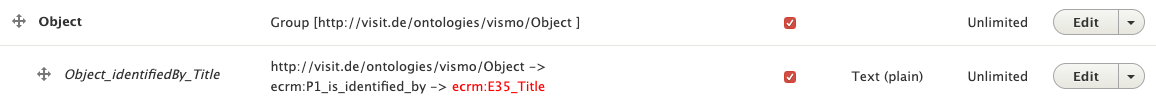
\includegraphics[width=\textwidth]{Figures/berndl/paths1}
    \caption{\label{fig:paths1} Zwei Beispiel-Pfade aus der \wisski Konfiguration des \visit Projekts.}
\end{figure}

Der zweite Pfade in \autoref{fig:paths1} ist nun ein wirklicher Pfad und steht high-level für den bezeichnenden Titel eines Ausstellungsobjekts. Die ID des Pfads ist \texttt{\q{Object\_identifiedBy\_Title}}, während der Pfad aus zwei Knoten und einer Relation besteht:

\begin{itemize}
	\item Da sich der Pfad bzw. der zugehörige Titel auf ein Ausstellungsobjekt beziehen soll, ist der erste Knoten von dem der Pfad ausgeht \texttt{\q{http://\-visit.\-de/\-ont\-o\-lo\-gies/\-vis\-mo/\-Ob\-ject}}.
	\item An diesen Knoten schließt sich dann die Relation \texttt{\q{ecrm:P1\_is\_i\-den\-ti\-fied\_by}} an.
	\item Der Zielknoten dieses Pfads ist ein weiterer Knoten: \texttt{\q{ecrm:E35\_Title}}.
\end{itemize}

Was für den zweiten Pfad noch fehlt ist der zugehörige Datentyp, welcher in der Ansicht in \autoref{fig:paths1} ebenfalls zu sehen ist: da ein Titel angegeben werden soll, definiert der Pfad eine Eigenschaft am Ende des Pfades (nicht in der Übersicht zu sehen) und benötigt damit einen primitiven Datentypen \texttt{\q{text/plain}}. Editiert man diesen Pfad, öffnet sich die Maske, die in \autoref{fig:pathsDetails1} zu sehen ist. Dort können viele Einstellungen zum Pfad editiert werden und zusätzlich ist die Angabe der letztendlichen Eigenschaft durch die Eingabe \texttt{\q{Datatype Property}} möglich. In diesem Beispiel ist der letzte Teil des Pfads somit \texttt{\q{http://erlangen-crm.org/170309/P3\_has\_note}}.

\begin{figure}[htb]
    \centering
    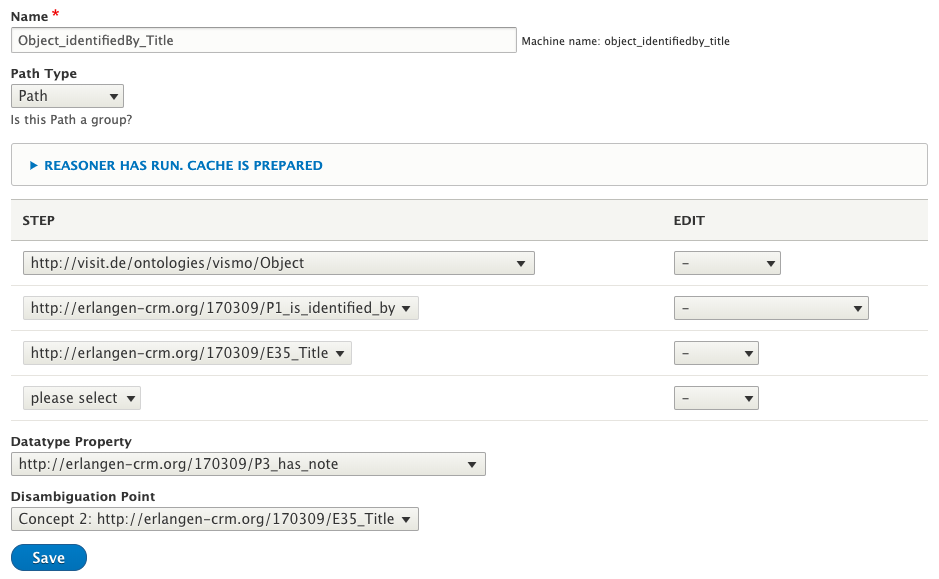
\includegraphics[width=\textwidth]{Figures/berndl/pathsDetails1}
    \caption{\label{fig:pathsDetails1} Erste Maske zum Editieren eines \wisski Pfads.}
\end{figure}

Wird die aktuelle Einstellung des Pfads gespeichert, öffnet sich die zweite Maske zur Konfiguration eines \wisski Pfads. Ausgehend von dem aktuellen Beispiel eines Objekt-Titels ist dies in \autoref{fig:pathsDetails2} zu sehen. Die ersten vier Einstellungen werden automatisch vom System gesetzt, und sollten in der Regel nicht angepasst werden müssen. Wichtig sind die vier unteren Einstellungen, welche den Datentypen des aktuell betrachteten Pfads definieren, indem zuerst der allgemeine Datentyp gesetzt wird und in den folgenden drei Einstellungen lässt sich einstellen, wie dieser Datentyp später in der Eingabemaske des \wisski Systems aussehen soll. In unserem Beispiel kann ein Text in einem einfachen Textfeld angelegt werden. Zusätzlich dazu kann die Kardinalität für das entsprechende Feld festgelegt werden.

\begin{figure}[htb]
    \centering
    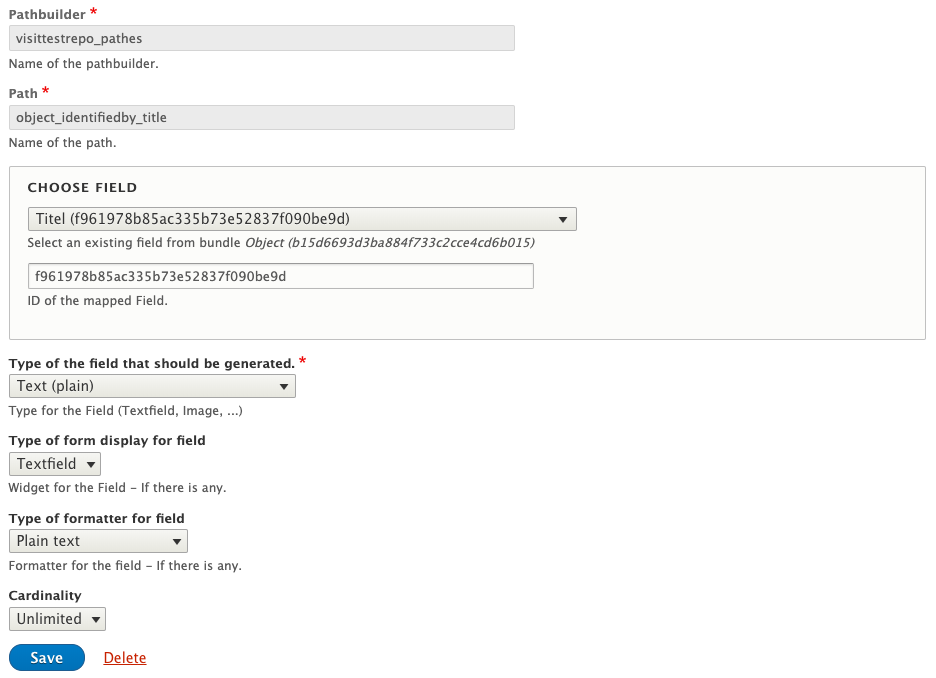
\includegraphics[width=\textwidth]{Figures/berndl/pathsDetails2}
    \caption{\label{fig:pathsDetails2} Zweite Maske zum Editieren eines \wisski Pfads.}
\end{figure}

\autoref{fig:paths2} zeigt weiterhin ein Beispiel für einen Pfad, welcher eine Relation zwischen zwei Datenbankobjekten definiert. In diesem Falle handelt es sich semantisch um eine Beziehung zwischen Teilobjekten, also dass ein Objekt ein Teil eines zweiten Objekts ist. Um dies zu tun ist der Datentyp \texttt{\q{Entity reference}} nötig, und dass der Pfad in der entsprechend zu referenzierenden Klasse endet: wie in diesem Fall \texttt{\q{http://\-visit.\-de/\-ont\-o\-lo\-gies/\-vis\-mo/\-Ob\-ject}}.

\begin{figure}[htb]
    \centering
    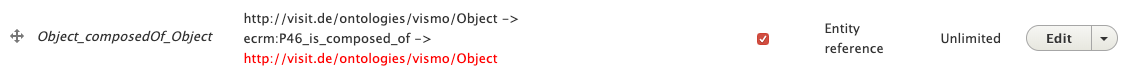
\includegraphics[width=\textwidth]{Figures/berndl/paths2}
    \caption{\label{fig:paths2} Beispiel-Pfad aus der \wisski Konfiguration des \visit Projekts für eine Relation zwischen zwei Entitäten der Datenbank.}
\end{figure}

Zwei weitere wichtige Punkte der \wisski Konfiguration sind in obigen Beispielen zu sehen:

\begin{description}
	\item[Anordnung der Pfade] Die Anordnung der Pfade spielt eine wichtige Rolle in der Konfiguration eines \wisski Systems. Dies ist auf der linken Seite in \autoref{fig:pathbuilder} und der Übersicht der Pfade eines Pathbuilders zu sehen. Die Pfade können dort (durch drag\&drop der \q{Kreuzchen} links neben einer Pfad-ID) in verschiedene Reihenfolgen bzw. Gruppierungen gebracht werden, um somit die Zugehörigkeit eines Pfads zu einer Gruppe, bzw. sogar einer Gruppe zu einer Obergruppe zu definieren. Dies wird getan, indem ein Pfad \q{unter} und dann \q{eine Ebene nach rechts} geschoben wird, wie dies im Beispiel für die ersten beiden Pfade zu sehen ist (ebenfalls in \autoref{fig:paths1} zu sehen). Eine Untergruppe zum Objekt bildet zum Beispiel der Pfad mit der ID \texttt{\q{Object\_Dating}}, welche ihrerseits wieder vier Pfade unter sich zusammen führt. Dies ist wichtig, da das Setzen eines dieser Pfade nicht jeweils einen eigenen Zwischenknoten (mit dem RDF Typen \texttt{\q{http://\-visit.\-de/\-ont\-o\-lo\-gies/\-vis\-mo/\-Da\-ting}}) erzeugen soll, sondern alle vier Pfade den selben Zwischenknoten benutzen sollen.
	\item[Disambiguierung] Die Disambiguierung bezieht sich - seicht formuliert - ähnlich wie die oben beschriebene Anordnung und Untergruppen indirekt auf die korrekte Zuweisung von Knoten zu ihren entsprechenden Objekten. Die Disambiguierung ist in den Pfaden durch die rot geschriebenen Teile zu sehen. Sie weißt das hinterliegende System an, dass alles was ab diesem Punkt im Pfad definiert ist, einzigartig im System gespeichert werden soll. Dadurch können keine Duplikate mit genau der selben Konfiguration entstehen. Dies lässt sich einfach am obigen Beispiel erläutern: die Disambiguierung für den Objekttitel beginnt ab dem \texttt{\q{ecrm:E35\_Title}} Knoten, der weiterhin nur die RDF Eigenschaft \texttt{\q{http://erlangen-crm.org/170309/P3\_has\_note}} besitzt. Durch die Disambiguierung an dieser Stelle wird das System keinen zweiten Knoten erstellen, der den selben Titel in der Notiz-Eigenschaft besitzt. Damit wird sichergestellt, dass zum Beispiel keine zwei Objekte mit dem Titel \q{Mona Lisa} erstellt werden können. Technisch verweist das System im Hintergrund bei verweis auf diesen Knoten somit immer auf genau diesen einen Knoten - wie beschrieben werden \textit{keine} Duplikate davon erstellt. Die Disambiguierung eines Pfads kann in der Maske mit dem Feld \texttt{\q{Disambiguation Point}} vorgenommen werden, die in \autoref{fig:pathsDetails1} zu sehen ist.
\end{description}

Die Informationen und die Konfiguration des Pathbuilders wird vom \wisski System weiterhin genutzt, um Ein- sowie Ausgabeinterfaces für die Hauptobjekte des Pathbuilders zu erzeugen. Über die Create-Seite des \wisski Systems (zu sehen in \autoref{fig:wisskiCreate} im Appendix) ist unter anderem das Eingabe-Interface für die Ausstellungsobjekte (Object) zu erreichen, dieses ist in \autoref{fig:wisskiCreateObject} im Appendix zu sehen. Nachdem Objekte über dieses erstellt wurden, können diese per Navigate- und Find-Seite des \wisski Systems eingesehen werden. Ein Beispiel für das Ausgabeinterface einer Partisane aus dem \visit Projekt ist in \autoref{fig:wisskiViewObject} im Appendix zu sehen.

\subsection{Technischer Zugang zu den Metadaten - die ViSIT REST API}\label{sec:rest}

Das oben beschriebene \wisski System ist entworfen, um im \visit Kontext Zugang für Geisteswissenschaftler, Museumsmitarbeiter und allgemein forschenden Personen zu schaffen. Weiterhin war es im \visit Projekt aber ebenfalls nötig, einen technischen Zugang zu den über \wisski erzeugten Daten zu gewährleisten. Diesen technischen Zugang verwenden weiter verarbeitende Komponenten des Projekts, beschrieben in den Kapiteln 4 bis 8. Ziel ist es ebenfalls, die Informationen der RDF Daten zu vermitteln, ohne dass der Empfänger mit RDF oder anderen semantischen Technologien in Berührung kommen muss.
% TODO insert \autoref{} bis \autoref{}.

Um dies auf standardisierte Weise durchzuführen, ist die Wahl auf eine serverseitige REST API gefallen, die mit den weiteren technischen Komponenten via HTTP kommunizieren kann. Die REST API ist in Java geschrieben und mit dem Spring Framework\footnote{\url{https://spring.io/}} umgesetzt. Die Entwicklung ist in einem Repository im allgemeinen \visit Projekt Bitbucket: \url{https://bitbucket.org/visit2016/metadb-rest-api/}. Eine direkte Kommunikation der aktuell installierten Version der REST API ist stets (sowohl auf dem produktiven Server als auch dem Testsystem) unter der URL Endung \texttt{\q{.../\-me\-ta\-d\-b-rest-api/\-swagger-ui.html}} zu finden.

Dieses Kapitel beschreibt weiterhin die allgemeine Umsetzung der API, dessen Hintergründe, sowie technische Eigenheiten wie Datenmodelle usw. Jedoch sind \textit{die wichtigsten technischen Details zur Verwendung der \visit REST API} in \autoref{sec:features} beschrieben. Dort werden unter anderem wichtige Skripte zur Inbetriebnahme der API erklärt, sowie der Prozess des Deployments erläutert.

Thematisch lässt sich die REST API in folgende Teile aufteilen, die unterschiedliche Aufgabenbereiche übernehmen:

\begin{description}
	\item[Digital Representations:] Die Digital Representations - zu deutsch digitale Repräsentationen - stellen die Verbindungen zwischen Metadaten und zugehörigen Mediendaten dar. Hierzu sind sie ein Eintrag in der Metadatenbank, die zu entsprechenden Entitäten hinzugefügt werden, und dabei verschiedene technische Details zu den Mediendaten beinhaltet. Die REST API bietet hierfür die Möglichkeiten, über HTTP entsprechende Digital Representations zu erzeugen, schreiben, bearbeiten, und zu löschen. Den Repräsentationen liegt folgendes (RDF) Modell, aufgezeigt in \autoref{fig:digrep}, zugrunde:
	
	\begin{figure}[htb]
    	\centering
	    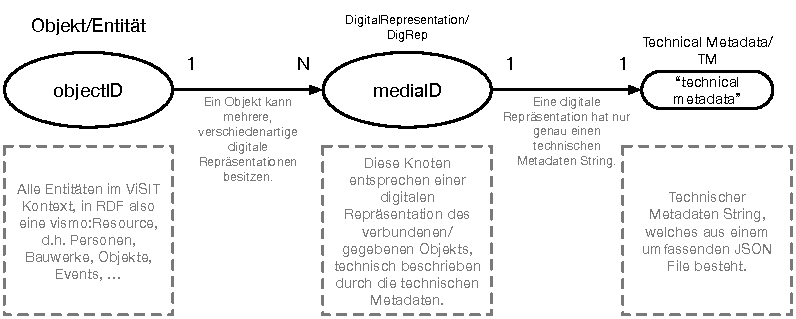
\includegraphics[width=\textwidth]{Figures/berndl/digrep}
    	\caption{\label{fig:digrep} Modell der digitalen Repräsentationen.}
	\end{figure}
	
	Die möglichen API Funktionen sind, in \autoref{tab:digrepapi} die folgenden (die API Pfade sind relativ zur jeweiligen REST API angegeben):
	
	\begin{table}[htb]
		\centering
		\begin{tabular}{|l|l|p{1.5cm}|p{5cm}|}
			\hline
			\texttt{HTTP} & \texttt{API Pfad} & \texttt{Request Params} & \texttt{Kurzbeschreibung} \\
			\hline
			\hline
			GET & /digrep/media & id & Gibt TM String des mit der \q{id} spezifizierten DigRep Knotens zurück. \\
			\hline
			PUT & /digrep/media & id, newData & Updated den TM String durch \q{newData} des per \q{id} spezifizierten DigRep Knotens. \\
			\hline
			DELETE & /digrep/media & id & Löscht den durch die \q{id} spezifizierten DigRep Knoten. \\
			\hline
			GET & /digrep/object & id & Gibt alle TM Strings und deren DigRep Knoten IDs zurück. \\
			\hline
			POST & /digrep/object & id & Legt einen neuen DigRep Knoten für das Objekt mit der gegebenen \q{id} an. \\
			\hline
			DELETE & /digrep/object & mediaId, objectId & Löscht den DigRep Knoten mit der ID \q{mediaID}, zugehörig zum Objekt mit der ID \q{objectID}. \\
			\hline
		\end{tabular}
		\caption{API Funktionen für die Digital Representations.}
		\label{tab:digrepapi}
	\end{table}

	\item[Objekte:] Dieser Bereich der API dient hauptsächlich zum Auslesen der Datenbankobjekte bzw. Entitäten, die über \wisski in der Metadatenbank angelegt wurden. Diese API Schnittstelle erfüllt die Anforderung, die bereits am Anfang dieses Unterkapitels beschrieben wurde: die Gewährleistung des technischen Auslesens der Metadaten in einem \textit{nicht}-Semantic Web Format, in diesem Falle JSON. Dieses JSON beinhaltet alle Informationen, die entsprechend als RDF Metadaten auf der Datenbank vorhanden sind. \autoref{lst:json} im Appendix gibt eine Art Schema für diesen Output an. Dort werden alle möglichen Felder mit ID, Datentyp und den potenziell referenzierten Typen einer Referenz angegeben. Zum Auslesen der Objekte bietet die API zwei mögliche API Funktionen aus \autoref{tab:objectapi}:
	
	\begin{table}[htb]
		\centering
		\begin{tabular}{|l|l|p{2cm}|p{5cm}|}
			\hline
			\texttt{HTTP} & \texttt{API Pfad} & \texttt{Request Params} & \texttt{Kurzbeschreibung} \\
			\hline
			\hline
			GET & /object & id & Gibt die JSON Repräsentation des Objekts mit der ID \q{id} zurück. \\
			\hline
			GET & /wisskiobject & wisskipath & Gibt die JSON Repräsentation des Objekts zurück, welches dem \wisski View Path \q{wisskipath} entspricht. \\
			\hline
		\end{tabular}
		\caption{API Funktionen zum Auslesen von Objekten.}
		\label{tab:objectapi}
	\end{table}
	
	Wichtig zu wissen beim Auslesen der Objekte ist, dass die angesprochene ID der API die RDF ID des Knotens der entsprechenden Entität ist (z.B. \texttt{\q{http://visit.de/data/5c4ae02a2d569}}), während der sogenannte \q{\wisski View Path} derjenige URL Pfad ist, der angezeigt wird, wenn eine Entität per \wisski Oberfläche betrachtet wird (z.B. \texttt{\q{https://\-da\-ta\-base.\-vi\-sit.\-u\-ni-pas\-sau.\-de/\-dru\-pal/\-wis\-ski/\-na\-vi\-gate/\-405/\-view}}).
	
	Weiterhin bietet dieser Bereich der API noch ein zusätzliches Quality of Life Feature: das Zurückgeben der Anzahl an vorhandenen Digital Representations und damit vorhandenen Mediendaten, bezogen auf ein Objekt. Dieses Objekt kann der API, wie beim Auslesen, per RDF ID oder per \wisski View Pfad übergeben werden.
	
	\item[(Upload und Download für Excel:)] TODO add?
\end{description}

Für die REST API ist eine Verschlüsselung umgesetzt, die dem Konzept der \q{basic authentication}\footnote{Erklärt z.B. auf \url{https://swagger.io/docs/specification/authentication/basic-authentication/}} folgt. Mit dieser werden die sogenannten \q{unsicheren} Operationen der API, also diejenigen, die Daten verändern, erzeugen, und löschen dürfen, von unzulässigem Zugriff geschützt. Diese sind im \visit Kontext diejenigen Operationen, die sich auf die DigitalRepresentations beziehen. Alle rein lesenden Zugriffe auf die Metadatenbank sind gemäß dem Linked Open Data Gedanken offen nach aussen.

Für die gesicherten Zugänge der API sind auf dem \visit Server verschiedene \q{User} samt Passwort angelegt, welche auf die jeweils verarbeitenden Applikationen gemünzt werden, dementsprechend die Tablet und Fernrohr Apps, sowie die Kompressions-Komponente. Diese Liste an Usern und Passwort sind am entsprechenden Server im eigenen Bereich des \q{visit} Accounts zu finden und nur für entsprechende Administratoren zugänglich. Die Datei hat den Namen \texttt{\q{users.csv}} und muss \textbf{vor dem Start bzw. dem Deployment} der REST API vorhanden sein, damit diese darauf Zugriff hat.

\subsection{Wichtige Technische Charakteristika der Entwicklung und den Betrieb der Semantischen Datenbank}\label{sec:features}

In diesem Unterabschnitt werden wichtige technische Details zum Betrieb der \visit REST API erläutert. Diese sind wichtig für die Nutzung der API.

\paragraph{Python Script zum Generieren der SPARQL Query Templates}

\textbf{WICHTIG:} Das im Folgenden beschriebene Script muss \textbf{vor} Deployment der REST API ausgeführt werden.

Für den Betrieb der REST API, vor allem zum Auslesen der unterliegenden Metadaten, sind sogenannte SPARQL Query Templates von Nöten. Diese können als Vorlagen für die Abfrage aus der Metadatenbank verstanden werden. Diese Query Templates werden automatisch aufbauend auf dem in \wisski definierten Paths erstellt. So kann, wenn sich die \wisski Pfad Konfiguration ändert, das Script erneut angestoßen werden, um auf die Veränderung zu reagieren und damit die neu hinzugefügten Pfade mit in die Anfragen aufgenommen werden. Dieser Prozess ist in einem Phyton Script gekapselt, welches auf dem \visit Server ausgeführt werden kann.

Wichtigste Information die das Script benötigt sind die Pfad Konfigurationen des \wisski Systems. Diese können als Datei direkt im \wisski System, im Pathbuilder downgeloadet werden. \autoref{fig:download} zeigt diese Funktionalität mit dem \texttt{\q{Create Exportfile}} Button.

	\begin{figure}[htb]
    	\centering
	    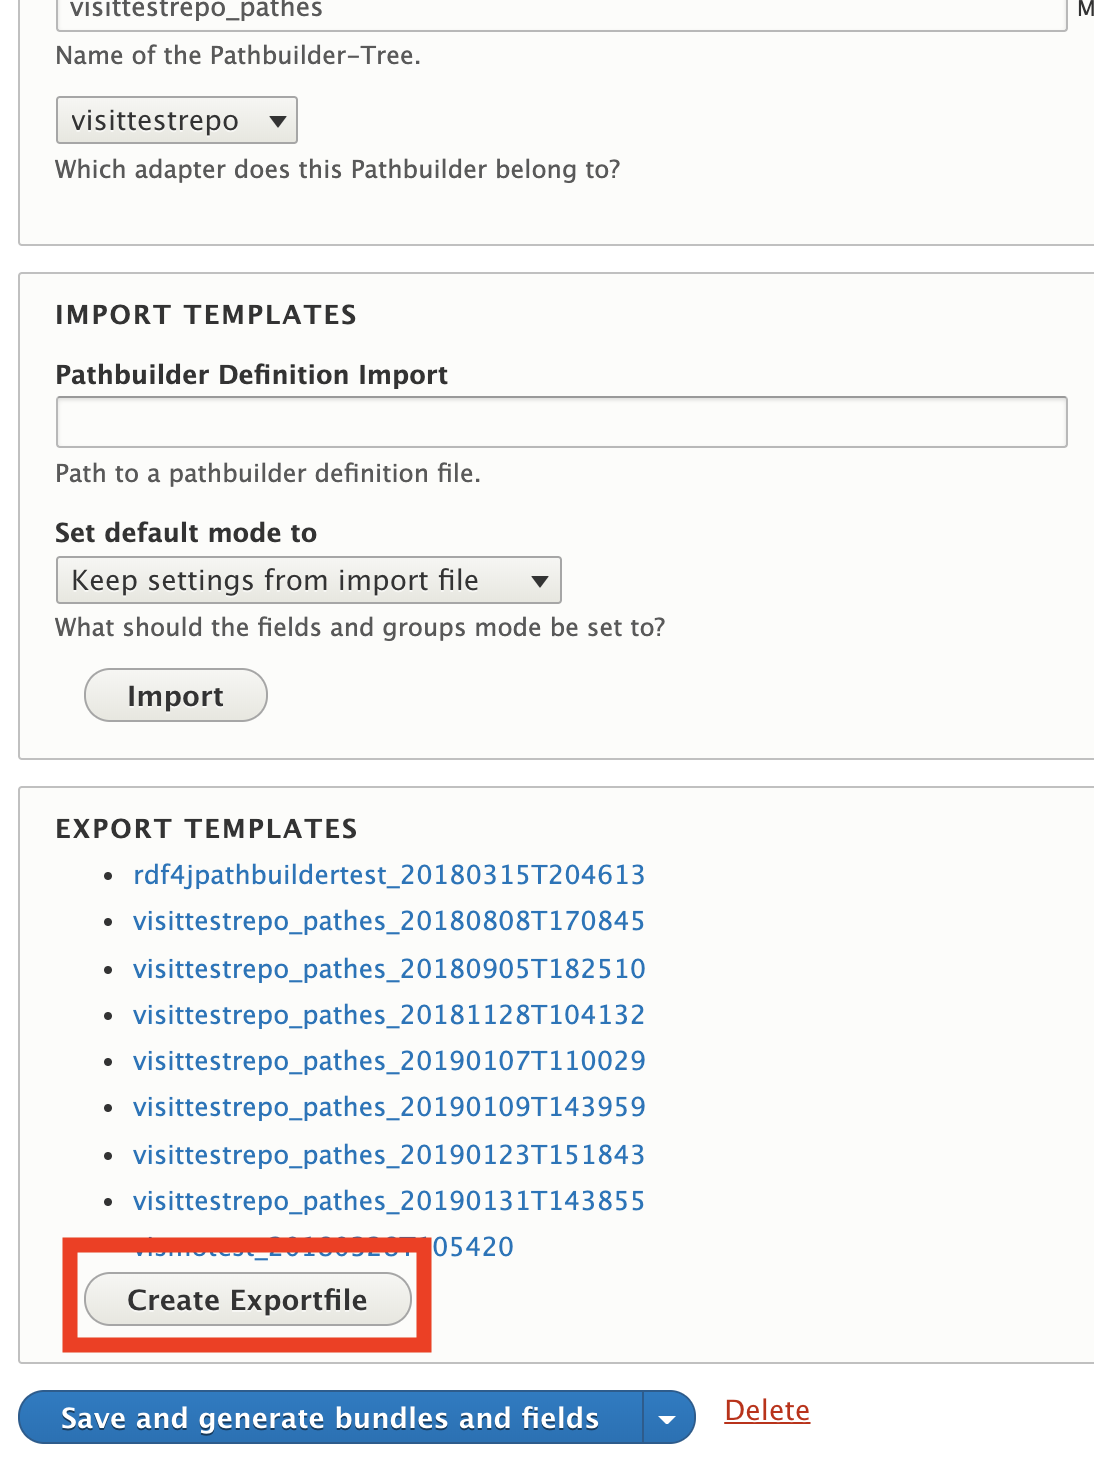
\includegraphics[width=\textwidth]{Figures/berndl/wisskiPathDownload}
    	\caption{\label{fig:download} \wisski Pathbuilder Ansicht, die den Download der Pfad-Datei anbietet.}
	\end{figure}
	
Nach Betätigen des Buttons wird eine aktuelle Datei in die darüber stehende Liste aufgenommen. Durch Drücken dieser kann die Datei anschließend gespeichert werden.

Das Python Script befindet sich auf dem Server im Account \texttt{\q{visit}} im Ordner \texttt{\q{python}} und heißt \texttt{\q{CreateSPARQLTemplatesFromPathsXML.py}}. \textbf{Die Pfad-Datei muss umbenannt werden zu \texttt{\q{paths.xml}} und muss sich im selben Ordner befinden}. Das Ausführen des Scripts kann mit folgendem Befehl ausgeführt werden:

\begin{lstlisting}[style=MyBashStyle, caption={Befehl zum Starten des Python Script zum Erstellen der Query Templates der \visit Metadatenbank.}]
sudo python3 CreateSPARQLTemplatesFromPathsXML.py
\end{lstlisting}

Die Ergebnisse des Scripts werden automatisch in den Ordner \texttt{\q{Templates}} im Hauptordner des Accounts \texttt{\q{visit}} gespeichert, und automatisiert von der REST API benutzt.

\paragraph{Einstellungen zum Deployment der REST API}

Wie oben bereits beschrieben, ist die REST API in einem Repository\footnote{\url{https://bitbucket.org/visit2016/metadb-rest-api/src/master/}} des \visit Haupt-Repositories angelegt.

In der Regel ist das entsprechende Projekt in einem \q{offline Teststatus} bezüglich seiner Konfiguration. Dies bedeutet, dass lokale Tests ausgeführt werden können, um die Funktionen der API lokal zu überprüfen. Sollte die REST API produktiv auf einem Server deployed werden, müssen folgende Änderungen in der Konfiguration durchgeführt werden:

\begin{itemize}
	\item Einbinden der springframework Dependency: In der \texttt{\q{pom.xml}} Maven Konfigurationsdatei des Projekts muss die Dependency für das Artefakt \texttt{\q{spring-boot-starter-tomcat}} auf den scope \texttt{\q{provided}} gesetzt werden. Die entsprechende Einstellung ist in \autoref{fig:springdependency} zu sehen. Wichtig ist, dass Zeile 4 \textbf{nicht} kommentiert ist.
	
	\begin{figure}[htb]
    	\centering
	    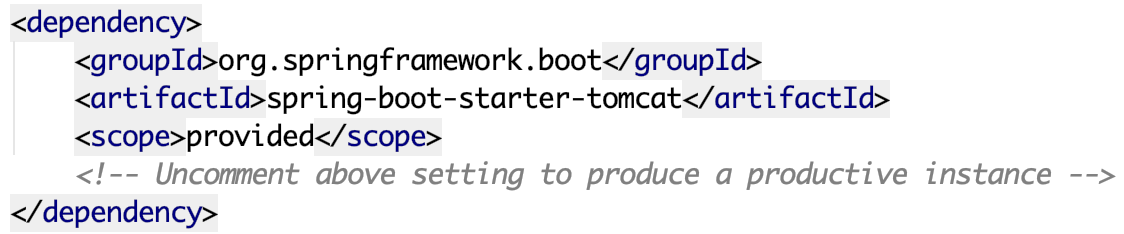
\includegraphics[width=\textwidth]{Figures/berndl/springDependency}
    	\caption{\label{fig:springdependency} pom.xml Konfiguration zum produktiven Deployment der REST API.}
	\end{figure}
	
	\item Verbindung zum entsprechenden Triplestore: Weiterhin ist es nötig, die REST API mit dem Triplestore zu verbinden, mit dem das aktuell verwendete System, im speziellen das \wisski System, arbeitet. Diese Verbindung wird in der REST API in der Konfigurationsdatei \texttt{\q{application.properties}} gesetzt. Dabei muss der query und der update Endpunkt URLs des jeweiligen Triplestores angegeben werden. Im offline Modus sind die beiden URLs auf \texttt{\q{none}} gesetzt, während sie für den Produktiv-Modus der API auf den entsprechenden Triplestore eingestellt werden müssen. In \autoref{fig:triplestoreconfig} ist die Konfiguration für den offline Modus zu sehen, während ebenfalls zwei vordefinierte URL Pärchen zu sehen sind, welche für den \visit Test- und Produktiv-Server stehen.
	
	\begin{figure}[htb]
    	\centering
	    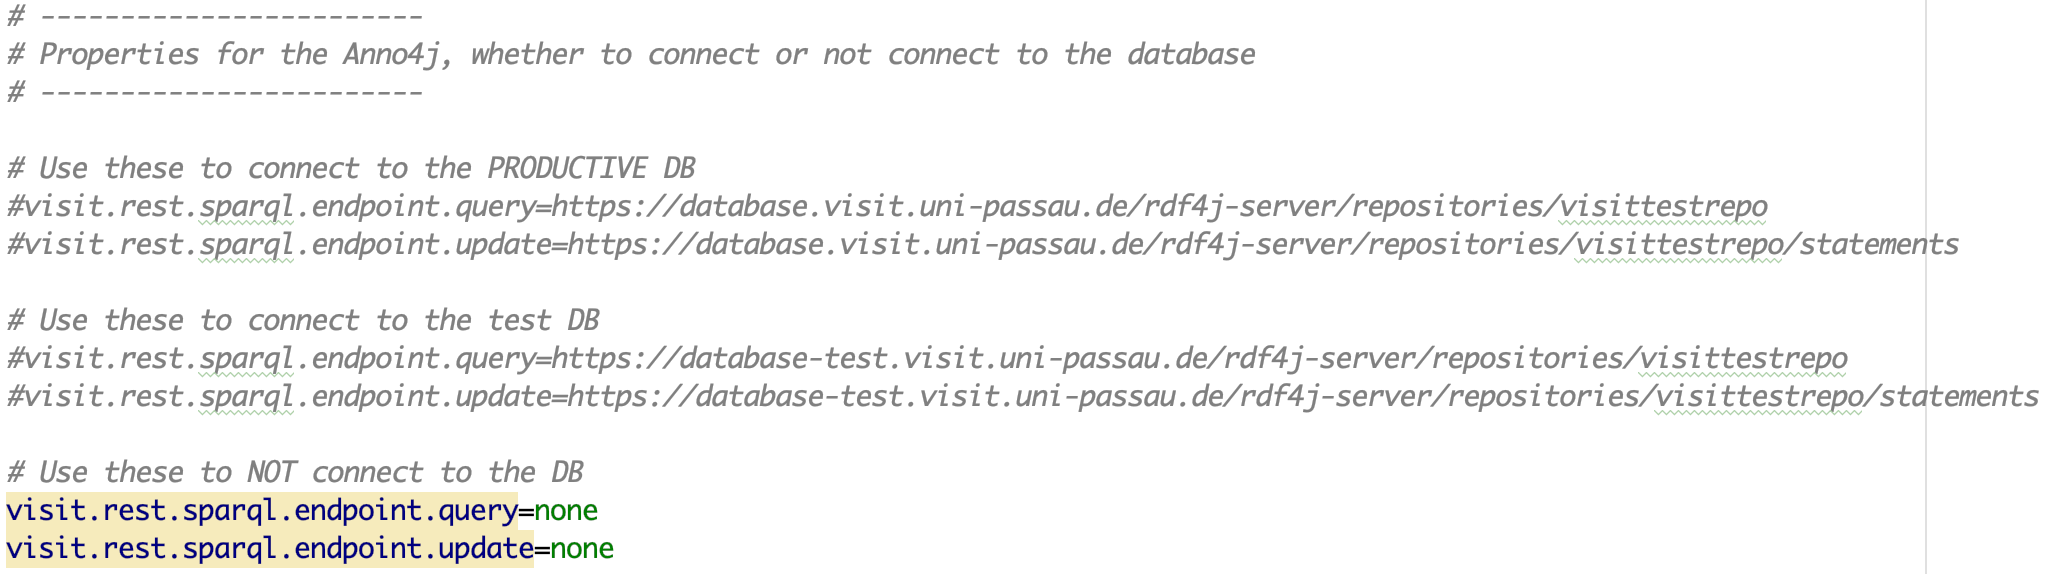
\includegraphics[width=\textwidth]{Figures/berndl/triplestoreConfig}
    	\caption{\label{fig:triplestoreconfig} Einstellungen zum Verbinden des Triplestores.}
	\end{figure}
\end{itemize}

\subsection{Zusatzfeatures - Erweiterung der Bedienbarkeit der Semantischen Datenbank}\label{sec:additional_features}

copy and paste feature

excel importer

\subsection{Semantische Datenbank - FAQ und häufig auftretende Probleme}\label{sec:faqSW}

generell gut: flush von wisski cashes sowie drupal per drush cc/cr

neue ontologie in wisski eingefügt: zum adapter gehen und recompute hierarchy

drupal update (manuell per hand und composer, manchmal per update dialog von drupal automatisch möglich)

seite schaltet sich selbst in maintenance mode -> meistens ein wichtiges drupal update -> drupal per composer updaten, dann sollte wieder gehen. wenn nicht, seite per drush aus maintenance nehmen, dann ist wieder zugreifbar

rdf4j zugriff: manchmal kommt der \q{connect to rdf4j Server} prompt, bevor man auf den triplestore kann. hier kann man normal nur \q{change} drücken, um fortzufahren. da die rdf4j jedoch lokal am server läuft, passt die URL oben nicht -> http auf https ändern, dann geht











\section{Schluss}\label{sec:schluss}

blub

\section{Appendix}\label{sec:appendix}

\begin{lstlisting}[caption={VisMo Ontologie in der letzten (englischen) Version.},label={lst:vismo},captionpos=b,language=xml]
<?xml version="1.0"?>
<rdf:RDF xmlns="http://visit.de/ontologies/vismo/"
     xml:base="http://visit.de/ontologies/vismo/"
     xmlns:rdf="http://www.w3.org/1999/02/22-rdf-syntax-ns#"
     xmlns:ns="http://www.w3.org/2003/06/sw-vocab-status/ns#"
     xmlns:owl="http://www.w3.org/2002/07/owl#"
     xmlns:xml="http://www.w3.org/XML/1998/namespace"
     xmlns:xsd="http://www.w3.org/2001/XMLSchema#"
     xmlns:skos="http://www.w3.org/2004/02/skos/core#"
     xmlns:rdfs="http://www.w3.org/2000/01/rdf-schema#"
     xmlns:wot="http://xmlns.com/wot/0.1/"
     xmlns:foaf="http://xmlns.com/foaf/0.1/"
     xmlns:dc="http://purl.org/dc/elements/1.1/">
    <owl:Ontology rdf:about="http://visit.de/ontologies/vismo/">
        <owl:versionIRI rdf:resource="http://visit.de/ontologies/vismo/0.4.5/"/>
        <owl:imports rdf:resource="http://erlangen-crm.org/170309/"/>
        <owl:imports rdf:resource="http://xmlns.com/foaf/0.1/"/>
    </owl:Ontology>
    


    <!-- 
    ///////////////////////////////////////////////////////////////////////////////////////
    //
    // Object Properties
    //
    ///////////////////////////////////////////////////////////////////////////////////////
     -->

    


    <!-- http://visit.de/ontologies/vismo/containsEntry -->

    <owl:ObjectProperty rdf:about="http://visit.de/ontologies/vismo/containsEntry">
        <rdfs:subPropertyOf rdf:resource="http://www.w3.org/2002/07/owl#topObjectProperty"/>
        <owl:inverseOf rdf:resource="http://visit.de/ontologies/vismo/isEntryIn"/>
        <rdfs:domain rdf:resource="http://visit.de/ontologies/vismo/Reference"/>
        <rdfs:range rdf:resource="http://visit.de/ontologies/vismo/ReferenceEntry"/>
        <rdfs:comment>Reference from a vismo:Reference to a contained vismo:ReferenceEntry.</rdfs:comment>
        <rdfs:label>contains entry</rdfs:label>
    </owl:ObjectProperty>
    


    <!-- http://visit.de/ontologies/vismo/employsTraderoute -->

    <owl:ObjectProperty rdf:about="http://visit.de/ontologies/vismo/employsTraderoute">
        <rdfs:subPropertyOf rdf:resource="http://www.w3.org/2002/07/owl#topObjectProperty"/>
        <owl:inverseOf rdf:resource="http://visit.de/ontologies/vismo/forTrade"/>
        <rdfs:domain rdf:resource="http://visit.de/ontologies/vismo/Trade"/>
        <rdfs:range rdf:resource="http://visit.de/ontologies/vismo/Traderoute"/>
        <rdfs:comment>Refers from a vismo:Trade to the vismo:TradeRoute that the trade is fullfilled on.</rdfs:comment>
        <rdfs:label>employs traderoute</rdfs:label>
    </owl:ObjectProperty>
    


    <!-- http://visit.de/ontologies/vismo/endLocation -->

    <owl:ObjectProperty rdf:about="http://visit.de/ontologies/vismo/endLocation">
        <rdfs:subPropertyOf rdf:resource="http://visit.de/ontologies/vismo/routeLocation"/>
        <rdfs:comment>Refers from a traderoute to the vismo:City that represents the ending point for the route.</rdfs:comment>
        <rdfs:label>end location</rdfs:label>
    </owl:ObjectProperty>
    


    <!-- http://visit.de/ontologies/vismo/entryIsAbout -->

    <owl:ObjectProperty rdf:about="http://visit.de/ontologies/vismo/entryIsAbout">
        <rdfs:subPropertyOf rdf:resource="http://www.w3.org/2002/07/owl#topObjectProperty"/>
        <owl:inverseOf rdf:resource="http://visit.de/ontologies/vismo/referencedByEntry"/>
        <rdfs:domain rdf:resource="http://visit.de/ontologies/vismo/ReferenceEntry"/>
        <rdfs:range rdf:resource="http://visit.de/ontologies/vismo/Resource"/>
        <rdfs:comment>Reference from a vismo:ReferenceEntry to a vismo:Resource, associating the describing nature of the associated vismo:Reference.</rdfs:comment>
        <rdfs:label>entry is about</rdfs:label>
    </owl:ObjectProperty>
    


    <!-- http://visit.de/ontologies/vismo/forTrade -->

    <owl:ObjectProperty rdf:about="http://visit.de/ontologies/vismo/forTrade">
        <rdfs:subPropertyOf rdf:resource="http://www.w3.org/2002/07/owl#topObjectProperty"/>
        <rdfs:domain rdf:resource="http://visit.de/ontologies/vismo/Traderoute"/>
        <rdfs:range rdf:resource="http://visit.de/ontologies/vismo/Trade"/>
        <rdfs:comment>Refers from a vismo:TradeRoute to the vismo:Trade resource that illustrates the trading on the given route.</rdfs:comment>
        <rdfs:label>for trade</rdfs:label>
    </owl:ObjectProperty>
    


    <!-- http://visit.de/ontologies/vismo/hasDigitalRepresentation -->

    <owl:ObjectProperty rdf:about="http://visit.de/ontologies/vismo/hasDigitalRepresentation">
        <rdfs:subPropertyOf rdf:resource="http://www.w3.org/2002/07/owl#topObjectProperty"/>
        <owl:inverseOf rdf:resource="http://visit.de/ontologies/vismo/representsDigitally"/>
        <rdfs:domain rdf:resource="http://visit.de/ontologies/vismo/Resource"/>
        <rdfs:range rdf:resource="http://visit.de/ontologies/vismo/DigitalRepresentation"/>
        <rdfs:comment>Links from a vismo:Resource (so an object that can be further specified in the ViSIT context) to a digital representation of it, e.g. a picture that shows the respective resource, a 3D model, etc.</rdfs:comment>
        <rdfs:label>has digital representation</rdfs:label>
    </owl:ObjectProperty>
    


    <!-- http://visit.de/ontologies/vismo/interactionSource -->

    <owl:ObjectProperty rdf:about="http://visit.de/ontologies/vismo/interactionSource">
        <rdfs:subPropertyOf rdf:resource="http://www.w3.org/2002/07/owl#topObjectProperty"/>
        <rdfs:domain rdf:resource="http://visit.de/ontologies/vismo/MiscellaneousInteraction"/>
        <rdfs:range rdf:resource="http://visit.de/ontologies/vismo/Resource"/>
        <rdfs:label>interaction source</rdfs:label>
    </owl:ObjectProperty>
    


    <!-- http://visit.de/ontologies/vismo/interactionTarget -->

    <owl:ObjectProperty rdf:about="http://visit.de/ontologies/vismo/interactionTarget">
        <rdfs:subPropertyOf rdf:resource="http://www.w3.org/2002/07/owl#topObjectProperty"/>
        <rdfs:domain rdf:resource="http://visit.de/ontologies/vismo/Resource"/>
        <rdfs:range rdf:resource="http://visit.de/ontologies/vismo/MiscellaneousInteraction"/>
        <rdfs:label>interaction target</rdfs:label>
    </owl:ObjectProperty>
    


    <!-- http://visit.de/ontologies/vismo/interstation -->

    <owl:ObjectProperty rdf:about="http://visit.de/ontologies/vismo/interstation">
        <rdfs:subPropertyOf rdf:resource="http://visit.de/ontologies/vismo/routeLocation"/>
        <rdfs:comment>Refers from a traderoute to the vismo:City that represents a interstation for the route.</rdfs:comment>
        <rdfs:label>interstation</rdfs:label>
    </owl:ObjectProperty>
    


    <!-- http://visit.de/ontologies/vismo/isEntryIn -->

    <owl:ObjectProperty rdf:about="http://visit.de/ontologies/vismo/isEntryIn">
        <rdfs:subPropertyOf rdf:resource="http://www.w3.org/2002/07/owl#topObjectProperty"/>
        <rdfs:domain rdf:resource="http://visit.de/ontologies/vismo/ReferenceEntry"/>
        <rdfs:range rdf:resource="http://visit.de/ontologies/vismo/Reference"/>
        <rdfs:comment>Reference from a vismo:ReferenceEntry to its encompassing vismo:Resource.</rdfs:comment>
        <rdfs:label>is entry in</rdfs:label>
    </owl:ObjectProperty>
    


    <!-- http://visit.de/ontologies/vismo/partOfTradeRoute -->

    <owl:ObjectProperty rdf:about="http://visit.de/ontologies/vismo/partOfTradeRoute">
        <rdfs:subPropertyOf rdf:resource="http://www.w3.org/2002/07/owl#topObjectProperty"/>
        <owl:inverseOf rdf:resource="http://visit.de/ontologies/vismo/routeLocation"/>
        <rdfs:domain rdf:resource="http://visit.de/ontologies/vismo/Place"/>
        <rdfs:range rdf:resource="http://visit.de/ontologies/vismo/Traderoute"/>
        <rdfs:comment>Refers from a vismo:City to a/multiple vismo:TradeRoute resource, indicating the given city is part of a trade route and therefore its associated trade.</rdfs:comment>
        <rdfs:label>part of trade route</rdfs:label>
    </owl:ObjectProperty>
    


    <!-- http://visit.de/ontologies/vismo/reference -->

    <owl:ObjectProperty rdf:about="http://visit.de/ontologies/vismo/reference">
        <rdfs:subPropertyOf rdf:resource="http://www.w3.org/2002/07/owl#topObjectProperty"/>
        <owl:inverseOf rdf:resource="http://visit.de/ontologies/vismo/referencedBy"/>
        <rdfs:domain rdf:resource="http://visit.de/ontologies/vismo/Resource"/>
        <rdfs:range rdf:resource="http://visit.de/ontologies/vismo/Reference"/>
        <rdfs:comment>Issues that the referenced vismo:Reference contains further and descriptive information about the given vismo:Resource entity.</rdfs:comment>
        <rdfs:label>reference</rdfs:label>
    </owl:ObjectProperty>
    


    <!-- http://visit.de/ontologies/vismo/referencedBy -->

    <owl:ObjectProperty rdf:about="http://visit.de/ontologies/vismo/referencedBy">
        <rdfs:subPropertyOf rdf:resource="http://www.w3.org/2002/07/owl#topObjectProperty"/>
        <rdfs:domain rdf:resource="http://visit.de/ontologies/vismo/Reference"/>
        <rdfs:range rdf:resource="http://visit.de/ontologies/vismo/Resource"/>
        <rdfs:comment>Refers to the vismo:Resource entities that reference this vismo:Reference and therefore this entity contains further and descriptive information about the resource entities.</rdfs:comment>
        <rdfs:label>referenced by</rdfs:label>
    </owl:ObjectProperty>
    


    <!-- http://visit.de/ontologies/vismo/referencedByEntry -->

    <owl:ObjectProperty rdf:about="http://visit.de/ontologies/vismo/referencedByEntry">
        <rdfs:subPropertyOf rdf:resource="http://www.w3.org/2002/07/owl#topObjectProperty"/>
        <rdfs:domain rdf:resource="http://visit.de/ontologies/vismo/Resource"/>
        <rdfs:range rdf:resource="http://visit.de/ontologies/vismo/ReferenceEntry"/>
        <rdfs:comment>Reference from a vismo:Resource to a given vismo:ReferenceEntry, indicating that the associated vismo:Reference contains information about the former.</rdfs:comment>
        <rdfs:label>referenced by entry</rdfs:label>
    </owl:ObjectProperty>
    


    <!-- http://visit.de/ontologies/vismo/representsDigitally -->

    <owl:ObjectProperty rdf:about="http://visit.de/ontologies/vismo/representsDigitally">
        <rdfs:subPropertyOf rdf:resource="http://www.w3.org/2002/07/owl#topObjectProperty"/>
        <rdfs:domain rdf:resource="http://visit.de/ontologies/vismo/DigitalRepresentation"/>
        <rdfs:range rdf:resource="http://visit.de/ontologies/vismo/Resource"/>
        <rdfs:comment>Refers from a given digital representation (a picture, 3D model, etc.) back to the vismo:Resource that it originally represents.</rdfs:comment>
        <rdfs:label>represents digitally</rdfs:label>
    </owl:ObjectProperty>
    


    <!-- http://visit.de/ontologies/vismo/routeLocation -->

    <owl:ObjectProperty rdf:about="http://visit.de/ontologies/vismo/routeLocation">
        <rdfs:subPropertyOf rdf:resource="http://www.w3.org/2002/07/owl#topObjectProperty"/>
        <rdfs:domain rdf:resource="http://visit.de/ontologies/vismo/Traderoute"/>
        <rdfs:range rdf:resource="http://visit.de/ontologies/vismo/Place"/>
        <rdfs:comment>Refers (with different sub-properties) from a vismo:TradeRoute to a vismo:City that is located on said route.</rdfs:comment>
        <rdfs:label>route location</rdfs:label>
    </owl:ObjectProperty>
    


    <!-- http://visit.de/ontologies/vismo/startLocation -->

    <owl:ObjectProperty rdf:about="http://visit.de/ontologies/vismo/startLocation">
        <rdfs:subPropertyOf rdf:resource="http://visit.de/ontologies/vismo/routeLocation"/>
        <rdfs:comment>Refers from a traderoute to the vismo:City that represents the starting point for the route.</rdfs:comment>
        <rdfs:label>start location</rdfs:label>
    </owl:ObjectProperty>
    


    <!-- 
    ///////////////////////////////////////////////////////////////////////////////////////
    //
    // Data properties
    //
    ///////////////////////////////////////////////////////////////////////////////////////
     -->

    


    <!-- http://visit.de/ontologies/vismo/buildingHistory -->

    <owl:DatatypeProperty rdf:about="http://visit.de/ontologies/vismo/buildingHistory">
        <rdfs:subPropertyOf rdf:resource="http://www.w3.org/2002/07/owl#topDataProperty"/>
        <rdfs:domain rdf:resource="http://visit.de/ontologies/vismo/Architecture"/>
        <rdfs:range rdf:resource="http://www.w3.org/2000/01/rdf-schema#Literal"/>
        <rdfs:comment>Property used to (freely) describe the building history of a vismo:Architecture entity.</rdfs:comment>
        <rdfs:label>building history</rdfs:label>
    </owl:DatatypeProperty>
    


    <!-- http://visit.de/ontologies/vismo/comment -->

    <owl:DatatypeProperty rdf:about="http://visit.de/ontologies/vismo/comment">
        <rdfs:subPropertyOf rdf:resource="http://www.w3.org/2002/07/owl#topDataProperty"/>
        <rdfs:domain rdf:resource="http://visit.de/ontologies/vismo/Resource"/>
        <rdfs:range rdf:resource="http://www.w3.org/2000/01/rdf-schema#Literal"/>
        <rdfs:comment rdf:datatype="http://www.w3.org/2001/XMLSchema#string">This is a comment about a given vismo entity.</rdfs:comment>
        <rdfs:isDefinedBy rdf:datatype="http://www.w3.org/2001/XMLSchema#string">http://visit.de/ontologies/vismo</rdfs:isDefinedBy>
        <rdfs:label rdf:datatype="http://www.w3.org/2001/XMLSchema#string">comment</rdfs:label>
    </owl:DatatypeProperty>
    


    <!-- http://visit.de/ontologies/vismo/description -->

    <owl:DatatypeProperty rdf:about="http://visit.de/ontologies/vismo/description">
        <rdfs:subPropertyOf rdf:resource="http://www.w3.org/2002/07/owl#topDataProperty"/>
        <rdfs:domain rdf:resource="http://visit.de/ontologies/vismo/Resource"/>
        <rdfs:range rdf:resource="http://www.w3.org/2000/01/rdf-schema#Literal"/>
        <rdfs:comment rdf:datatype="http://www.w3.org/2001/XMLSchema#string">This property defines a (historical) description for a vismo entity.</rdfs:comment>
        <rdfs:isDefinedBy rdf:datatype="http://www.w3.org/2001/XMLSchema#string">http://visit.de/ontologies/vismo/</rdfs:isDefinedBy>
        <rdfs:label rdf:datatype="http://www.w3.org/2001/XMLSchema#string">description</rdfs:label>
    </owl:DatatypeProperty>
    


    <!-- http://visit.de/ontologies/vismo/entryPages -->

    <owl:DatatypeProperty rdf:about="http://visit.de/ontologies/vismo/entryPages">
        <rdfs:subPropertyOf rdf:resource="http://www.w3.org/2002/07/owl#topDataProperty"/>
        <rdfs:domain rdf:resource="http://visit.de/ontologies/vismo/ReferenceEntry"/>
        <rdfs:range rdf:resource="http://www.w3.org/2000/01/rdf-schema#Literal"/>
        <rdfs:comment>The range of pages that a given vismo:ReferenceEntry references of a vismo:Reference entity.</rdfs:comment>
        <rdfs:label>entry pages</rdfs:label>
    </owl:DatatypeProperty>
    


    <!-- http://visit.de/ontologies/vismo/helpfulLinks -->

    <owl:DatatypeProperty rdf:about="http://visit.de/ontologies/vismo/helpfulLinks">
        <rdfs:subPropertyOf rdf:resource="http://www.w3.org/2002/07/owl#topDataProperty"/>
        <rdfs:domain rdf:resource="http://visit.de/ontologies/vismo/Resource"/>
        <rdfs:range rdf:resource="http://www.w3.org/2000/01/rdf-schema#Literal"/>
        <rdfs:comment>This property is used to conveniently collect links to online resources that contain further information of the associated vismo:Resource.</rdfs:comment>
        <rdfs:label>helpful links</rdfs:label>
    </owl:DatatypeProperty>
    


    <!-- http://visit.de/ontologies/vismo/iconography -->

    <owl:DatatypeProperty rdf:about="http://visit.de/ontologies/vismo/iconography">
        <rdfs:subPropertyOf rdf:resource="http://www.w3.org/2002/07/owl#topDataProperty"/>
        <rdfs:domain rdf:resource="http://visit.de/ontologies/vismo/Resource"/>
        <rdfs:range rdf:resource="http://www.w3.org/2000/01/rdf-schema#Literal"/>
        <rdfs:comment>A property to associate iconography to a given vismo:Resource entity.</rdfs:comment>
        <rdfs:label>iconography</rdfs:label>
    </owl:DatatypeProperty>
    


    <!-- http://visit.de/ontologies/vismo/innerDescription -->

    <owl:DatatypeProperty rdf:about="http://visit.de/ontologies/vismo/innerDescription">
        <rdfs:subPropertyOf rdf:resource="http://www.w3.org/2002/07/owl#topDataProperty"/>
        <rdfs:domain rdf:resource="http://visit.de/ontologies/vismo/Architecture"/>
        <rdfs:range rdf:resource="http://www.w3.org/2000/01/rdf-schema#Literal"/>
        <rdfs:comment>Property used to describe the interior of a vismo:Architecture entity.</rdfs:comment>
        <rdfs:label>inner description</rdfs:label>
    </owl:DatatypeProperty>
    


    <!-- http://visit.de/ontologies/vismo/keyword -->

    <owl:DatatypeProperty rdf:about="http://visit.de/ontologies/vismo/keyword">
        <rdfs:subPropertyOf rdf:resource="http://www.w3.org/2002/07/owl#topDataProperty"/>
        <rdfs:domain rdf:resource="http://visit.de/ontologies/vismo/Resource"/>
        <rdfs:range rdf:resource="http://www.w3.org/2000/01/rdf-schema#Literal"/>
        <rdfs:comment>This property is used to address keywords for a vismo:Resource entity. These refer to more general topics that can be addressed to anything out of the VisMo domain, for example &quot;Trade&quot;, &quot;War&quot;/&quot;Peace&quot;, or overall temporal associations.</rdfs:comment>
        <rdfs:label>keyword</rdfs:label>
    </owl:DatatypeProperty>
    


    <!-- http://visit.de/ontologies/vismo/literature -->

    <owl:DatatypeProperty rdf:about="http://visit.de/ontologies/vismo/literature">
        <rdfs:subPropertyOf rdf:resource="http://www.w3.org/2002/07/owl#topDataProperty"/>
        <rdfs:domain rdf:resource="http://visit.de/ontologies/vismo/Resource"/>
        <rdfs:range rdf:resource="http://www.w3.org/2000/01/rdf-schema#Literal"/>
        <rdfs:comment rdf:datatype="http://www.w3.org/2001/XMLSchema#string">This property defines a literature entry that contains further information about the given vismo entity.</rdfs:comment>
        <rdfs:isDefinedBy rdf:datatype="http://www.w3.org/2001/XMLSchema#string">http://visit.de/ontologies/vismo/</rdfs:isDefinedBy>
        <rdfs:label rdf:datatype="http://www.w3.org/2001/XMLSchema#string">literature</rdfs:label>
    </owl:DatatypeProperty>
    


    <!-- http://visit.de/ontologies/vismo/outerDescription -->

    <owl:DatatypeProperty rdf:about="http://visit.de/ontologies/vismo/outerDescription">
        <rdfs:subPropertyOf rdf:resource="http://www.w3.org/2002/07/owl#topDataProperty"/>
        <rdfs:domain rdf:resource="http://visit.de/ontologies/vismo/Architecture"/>
        <rdfs:range rdf:resource="http://www.w3.org/2000/01/rdf-schema#Literal"/>
        <rdfs:comment>Property used to describe the exterior of a vismo:Architecture entity.</rdfs:comment>
        <rdfs:label>outer description</rdfs:label>
    </owl:DatatypeProperty>
    


    <!-- http://visit.de/ontologies/vismo/pages -->

    <owl:DatatypeProperty rdf:about="http://visit.de/ontologies/vismo/pages">
        <rdfs:subPropertyOf rdf:resource="http://www.w3.org/2002/07/owl#topDataProperty"/>
        <rdfs:domain rdf:resource="http://visit.de/ontologies/vismo/Reference"/>
        <rdfs:range rdf:resource="http://www.w3.org/2000/01/rdf-schema#Literal"/>
        <rdfs:comment>Number of pages of a given vismo:Reference entity.</rdfs:comment>
        <rdfs:label>pages</rdfs:label>
    </owl:DatatypeProperty>
    


    <!-- http://visit.de/ontologies/vismo/publisher -->

    <owl:DatatypeProperty rdf:about="http://visit.de/ontologies/vismo/publisher">
        <rdfs:subPropertyOf rdf:resource="http://www.w3.org/2002/07/owl#topDataProperty"/>
        <rdfs:domain rdf:resource="http://visit.de/ontologies/vismo/Reference"/>
        <rdfs:range rdf:resource="http://www.w3.org/2000/01/rdf-schema#Literal"/>
        <rdfs:comment>The publisher of the given vismo:Reference entity.</rdfs:comment>
        <rdfs:label>publisher</rdfs:label>
    </owl:DatatypeProperty>
    


    <!-- http://visit.de/ontologies/vismo/series -->

    <owl:DatatypeProperty rdf:about="http://visit.de/ontologies/vismo/series">
        <rdfs:subPropertyOf rdf:resource="http://www.w3.org/2002/07/owl#topDataProperty"/>
        <rdfs:domain rdf:resource="http://visit.de/ontologies/vismo/Reference"/>
        <rdfs:range rdf:resource="http://www.w3.org/2000/01/rdf-schema#Literal"/>
        <rdfs:label>series</rdfs:label>
    </owl:DatatypeProperty>
    


    <!-- http://visit.de/ontologies/vismo/superordinateTitle -->

    <owl:DatatypeProperty rdf:about="http://visit.de/ontologies/vismo/superordinateTitle">
        <rdfs:subPropertyOf rdf:resource="http://www.w3.org/2002/07/owl#topDataProperty"/>
        <rdfs:domain rdf:resource="http://visit.de/ontologies/vismo/Title"/>
        <rdfs:range rdf:resource="http://www.w3.org/2000/01/rdf-schema#Literal"/>
        <rdfs:comment>Textual String to name the title of the superordinate reference collection that incorporates the associated vismo:Reference entity.</rdfs:comment>
        <rdfs:label>superordinate title</rdfs:label>
    </owl:DatatypeProperty>
    


    <!-- http://visit.de/ontologies/vismo/technicalMetadata -->

    <owl:DatatypeProperty rdf:about="http://visit.de/ontologies/vismo/technicalMetadata">
        <rdfs:subPropertyOf rdf:resource="http://www.w3.org/2002/07/owl#topDataProperty"/>
        <rdfs:domain rdf:resource="http://visit.de/ontologies/vismo/DigitalRepresentation"/>
        <rdfs:range rdf:resource="http://www.w3.org/2000/01/rdf-schema#Literal"/>
        <rdfs:comment>Refers from a vismo:DigitalRepresentation to a JSON formatted String that represents the technical metadata that is produced by the process that creates given digital representation.</rdfs:comment>
        <rdfs:label>technical metadata</rdfs:label>
    </owl:DatatypeProperty>
    


    <!-- http://visit.de/ontologies/vismo/thumbnail -->

    <owl:DatatypeProperty rdf:about="http://visit.de/ontologies/vismo/thumbnail">
        <rdfs:subPropertyOf rdf:resource="http://www.w3.org/2002/07/owl#topDataProperty"/>
        <rdfs:domain rdf:resource="http://visit.de/ontologies/vismo/Resource"/>
        <rdfs:range rdf:resource="http://www.w3.org/2000/01/rdf-schema#Literal"/>
        <rdfs:comment>A thumbnail generated for the respective digital representation. In general a base 64 encoding.</rdfs:comment>
        <rdfs:label>thumbnail</rdfs:label>
    </owl:DatatypeProperty>
    


    <!-- http://visit.de/ontologies/vismo/volume -->

    <owl:DatatypeProperty rdf:about="http://visit.de/ontologies/vismo/volume">
        <rdfs:subPropertyOf rdf:resource="http://www.w3.org/2002/07/owl#topDataProperty"/>
        <rdfs:domain rdf:resource="http://visit.de/ontologies/vismo/Reference"/>
        <rdfs:range rdf:resource="http://www.w3.org/2000/01/rdf-schema#Literal"/>
        <rdfs:comment>Number of volumes of a given publication series.</rdfs:comment>
        <rdfs:label>volume</rdfs:label>
    </owl:DatatypeProperty>
    


    <!-- http://www.w3.org/2002/07/owl#topDataProperty -->

    <rdf:Description rdf:about="http://www.w3.org/2002/07/owl#topDataProperty">
        <rdfs:domain rdf:resource="http://visit.de/ontologies/vismo/DigitalRepresentation"/>
        <rdfs:range rdf:resource="http://www.w3.org/2000/01/rdf-schema#Literal"/>
    </rdf:Description>
    


    <!-- 
    ///////////////////////////////////////////////////////////////////////////////////////
    //
    // Classes
    //
    ///////////////////////////////////////////////////////////////////////////////////////
     -->

    


    <!-- http://visit.de/ontologies/vismo/Activity -->

    <owl:Class rdf:about="http://visit.de/ontologies/vismo/Activity">
        <rdfs:subClassOf rdf:resource="http://erlangen-crm.org/170309/E7_Activity"/>
        <rdfs:subClassOf rdf:resource="http://visit.de/ontologies/vismo/Resource"/>
        <rdfs:comment>Activities in the ViSIT context are any type of timely historical event that can contribute a timely frame for associated ViSIT concepts. For example &quot;World War II&quot;, &quot;The battle for town x&quot;, etc.</rdfs:comment>
        <rdfs:label>Activity</rdfs:label>
    </owl:Class>
    


    <!-- http://visit.de/ontologies/vismo/Architecture -->

    <owl:Class rdf:about="http://visit.de/ontologies/vismo/Architecture">
        <rdfs:subClassOf rdf:resource="http://erlangen-crm.org/170309/E53_Place"/>
        <rdfs:subClassOf rdf:resource="http://erlangen-crm.org/170309/E84_Information_Carrier"/>
        <rdfs:subClassOf rdf:resource="http://visit.de/ontologies/vismo/Resource"/>
        <rdfs:comment>Architecture in the ViSIT context describes every building or architectural production that has been erected by mankind in some way.</rdfs:comment>
        <rdfs:label>Architecture</rdfs:label>
    </owl:Class>
    


    <!-- http://visit.de/ontologies/vismo/BishopricAffiliation -->

    <owl:Class rdf:about="http://visit.de/ontologies/vismo/BishopricAffiliation">
        <rdfs:subClassOf rdf:resource="http://erlangen-crm.org/170309/E55_Type"/>
        <rdfs:comment>This class comprises headwords for bishopric affiliations for vismo:Architecture resources.</rdfs:comment>
        <rdfs:label>Bishopric Affiliation</rdfs:label>
    </owl:Class>
    


    <!-- http://visit.de/ontologies/vismo/Country -->

    <owl:Class rdf:about="http://visit.de/ontologies/vismo/Country">
        <rdfs:subClassOf rdf:resource="http://erlangen-crm.org/170309/E53_Place"/>
        <rdfs:subClassOf rdf:resource="http://visit.de/ontologies/vismo/Resource"/>
        <rdfs:label>Country</rdfs:label>
    </owl:Class>
    


    <!-- http://visit.de/ontologies/vismo/Dating -->

    <owl:Class rdf:about="http://visit.de/ontologies/vismo/Dating">
        <rdfs:subClassOf rdf:resource="http://erlangen-crm.org/170309/E52_Time-Span"/>
        <rdfs:comment>More specific class of the E52_TimeSpan and used in the ViSIT context to give temporal associations with various entities.</rdfs:comment>
        <rdfs:label>Dating</rdfs:label>
    </owl:Class>
    


    <!-- http://visit.de/ontologies/vismo/Description -->

    <owl:Class rdf:about="http://visit.de/ontologies/vismo/Description">
        <rdfs:subClassOf rdf:resource="http://erlangen-crm.org/170309/E55_Type"/>
        <rdfs:comment>Descriptions comprise characteristic types for objects in the domain of museums. Therefore these are for example &quot;painting&quot;, &quot;oil painting&quot;, &quot;chest&quot;, etc.</rdfs:comment>
        <rdfs:label>Description</rdfs:label>
    </owl:Class>
    


    <!-- http://visit.de/ontologies/vismo/DigitalRepresentation -->

    <owl:Class rdf:about="http://visit.de/ontologies/vismo/DigitalRepresentation">
        <rdfs:subClassOf rdf:resource="http://www.w3.org/2000/01/rdf-schema#Class"/>
        <rdfs:comment>A digital representation symbolises a multimedia representation of a vismo:Resource that can be illustrated in some way. These incorporate pictures, videos, audio files, and 3D models in particular.</rdfs:comment>
        <rdfs:label>Digital Representation</rdfs:label>
    </owl:Class>
    


    <!-- http://visit.de/ontologies/vismo/Function -->

    <owl:Class rdf:about="http://visit.de/ontologies/vismo/Function">
        <rdfs:subClassOf rdf:resource="http://erlangen-crm.org/170309/E55_Type"/>
        <rdfs:comment>Functions relate to semantical and functional properties that are inherited by vismo:Object as well as vismo:Architecture and their vismo:Structural Evolution resources. Both an object as well as an architecture could exert &quot;military&quot; functions.</rdfs:comment>
        <rdfs:label>Function</rdfs:label>
    </owl:Class>
    


    <!-- http://visit.de/ontologies/vismo/GeographicalAffiliation -->

    <owl:Class rdf:about="http://visit.de/ontologies/vismo/GeographicalAffiliation">
        <rdfs:subClassOf rdf:resource="http://erlangen-crm.org/170309/E55_Type"/>
        <rdfs:comment>This class comprises headwords for geographical affiliations for vismo:Architecture resources.</rdfs:comment>
        <rdfs:label>Geographical Affiliation</rdfs:label>
    </owl:Class>
    


    <!-- http://visit.de/ontologies/vismo/Group -->

    <owl:Class rdf:about="http://visit.de/ontologies/vismo/Group">
        <rdfs:subClassOf rdf:resource="http://erlangen-crm.org/170309/E74_Group"/>
        <rdfs:subClassOf rdf:resource="http://visit.de/ontologies/vismo/Resource"/>
        <rdfs:comment>This more general class will comprise different groups of people that are associated in the VisMo context. In the first instance these are WorkingGroups (Werkst\"a tten) and joint practices (Soziet\"a ten).</rdfs:comment>
        <rdfs:label>Group</rdfs:label>
    </owl:Class>
    


    <!-- http://visit.de/ontologies/vismo/GroupDescription -->

    <owl:Class rdf:about="http://visit.de/ontologies/vismo/GroupDescription">
        <rdfs:subClassOf rdf:resource="http://erlangen-crm.org/170309/E55_Type"/>
        <rdfs:comment>This Class comprises descriptional types for all kinds of groups that are associated in the VisMo context, such as Werkstatt and Soziet\"a t.</rdfs:comment>
        <rdfs:label>Group Description</rdfs:label>
    </owl:Class>
    


    <!-- http://visit.de/ontologies/vismo/HistoricalChange -->

    <owl:Class rdf:about="http://visit.de/ontologies/vismo/HistoricalChange">
        <rdfs:subClassOf rdf:resource="http://erlangen-crm.org/170309/E9_Move"/>
        <rdfs:subClassOf rdf:resource="http://visit.de/ontologies/vismo/Resource"/>
        <rdfs:label>HistoricalChange</rdfs:label>
    </owl:Class>
    


    <!-- http://visit.de/ontologies/vismo/InscriptionType -->

    <owl:Class rdf:about="http://visit.de/ontologies/vismo/InscriptionType">
        <rdfs:subClassOf rdf:resource="http://erlangen-crm.org/170309/E55_Type"/>
        <rdfs:comment>This E55_Type describes the type of an Inscription, done on various vismo:Object entities.</rdfs:comment>
        <rdfs:label>Inscription Type</rdfs:label>
    </owl:Class>
    


    <!-- http://visit.de/ontologies/vismo/Institution -->

    <owl:Class rdf:about="http://visit.de/ontologies/vismo/Institution">
        <rdfs:subClassOf rdf:resource="http://erlangen-crm.org/170309/E53_Place"/>
        <rdfs:subClassOf rdf:resource="http://erlangen-crm.org/170309/E74_Group"/>
        <rdfs:subClassOf rdf:resource="http://visit.de/ontologies/vismo/Resource"/>
        <rdfs:comment>An institution in the ViSIT context is primarily used for museums, which inherit both the properties of a E53_Place as well as a E74_Group. This is necessary to make instances of this class be able to represent a spatial entity as well as an entity that can for example hold vismo:Objects.</rdfs:comment>
        <rdfs:label>Institution</rdfs:label>
    </owl:Class>
    


    <!-- http://visit.de/ontologies/vismo/Marriage -->

    <owl:Class rdf:about="http://visit.de/ontologies/vismo/Marriage">
        <rdfs:subClassOf rdf:resource="http://erlangen-crm.org/170309/E74_Group"/>
        <rdfs:subClassOf rdf:resource="http://visit.de/ontologies/vismo/Resource"/>
        <rdfs:comment>A Subclass of the E74_Group in order to differentiate the participation of a vismo:Person in a Marriage rather than any other vismo:Group.</rdfs:comment>
        <rdfs:label>Marriage</rdfs:label>
    </owl:Class>
    


    <!-- http://visit.de/ontologies/vismo/MiscellaneousInteraction -->

    <owl:Class rdf:about="http://visit.de/ontologies/vismo/MiscellaneousInteraction">
        <rdfs:subClassOf rdf:resource="http://erlangen-crm.org/170309/E7_Activity"/>
        <rdfs:subClassOf rdf:resource="http://visit.de/ontologies/vismo/Resource"/>
        <rdfs:comment>This E7_Activity subclass is used for various dynamic interactions between vismo:Resource objects, whose interaction is not yet known or more specifically not defined by the ontology model.</rdfs:comment>
        <rdfs:label>MiscellaneousInteraction</rdfs:label>
    </owl:Class>
    


    <!-- http://visit.de/ontologies/vismo/Mounting -->

    <owl:Class rdf:about="http://visit.de/ontologies/vismo/Mounting">
        <rdfs:subClassOf rdf:resource="http://erlangen-crm.org/170309/E55_Type"/>
        <rdfs:comment>This class comprises the various possibilities of fix/mount/place an Inscription onto a vismo:Object.</rdfs:comment>
        <rdfs:label>Mounting</rdfs:label>
    </owl:Class>
    


    <!-- http://visit.de/ontologies/vismo/Object -->

    <owl:Class rdf:about="http://visit.de/ontologies/vismo/Object">
        <rdfs:subClassOf rdf:resource="http://erlangen-crm.org/170309/E84_Information_Carrier"/>
        <rdfs:subClassOf rdf:resource="http://visit.de/ontologies/vismo/Resource"/>
        <rdfs:comment>Objects in the ViSIT context subsume all sorts of items that are displayed in a museum.</rdfs:comment>
        <rdfs:label>Object</rdfs:label>
    </owl:Class>
    


    <!-- http://visit.de/ontologies/vismo/OrderAffiliation -->

    <owl:Class rdf:about="http://visit.de/ontologies/vismo/OrderAffiliation">
        <rdfs:subClassOf rdf:resource="http://erlangen-crm.org/170309/E55_Type"/>
        <rdfs:comment>This class comprises headwords for order affiliations for vismo:Architecture resources.</rdfs:comment>
        <rdfs:label>Order Affiliation</rdfs:label>
    </owl:Class>
    


    <!-- http://visit.de/ontologies/vismo/Person -->

    <owl:Class rdf:about="http://visit.de/ontologies/vismo/Person">
        <rdfs:subClassOf rdf:resource="http://erlangen-crm.org/170309/E21_Person"/>
        <rdfs:subClassOf rdf:resource="http://visit.de/ontologies/vismo/Resource"/>
        <rdfs:subClassOf rdf:resource="http://xmlns.com/foaf/0.1/Person"/>
        <rdfs:label>Person</rdfs:label>
    </owl:Class>
    


    <!-- http://visit.de/ontologies/vismo/Place -->

    <owl:Class rdf:about="http://visit.de/ontologies/vismo/Place">
        <rdfs:subClassOf rdf:resource="http://erlangen-crm.org/170309/E53_Place"/>
        <rdfs:subClassOf rdf:resource="http://visit.de/ontologies/vismo/Resource"/>
        <rdfs:comment>All cities, towns, settlements etc. of some sort are subsumed under this class.</rdfs:comment>
        <rdfs:label>Place</rdfs:label>
    </owl:Class>
    


    <!-- http://visit.de/ontologies/vismo/Profession -->

    <owl:Class rdf:about="http://visit.de/ontologies/vismo/Profession">
        <rdfs:subClassOf rdf:resource="http://erlangen-crm.org/170309/E55_Type"/>
        <rdfs:comment>Professions subsume all roles, employments, titles, authorities, etc. for persons that are inherent in the cultural heritage domain.</rdfs:comment>
        <rdfs:label>Profession</rdfs:label>
    </owl:Class>
    


    <!-- http://visit.de/ontologies/vismo/Reference -->

    <owl:Class rdf:about="http://visit.de/ontologies/vismo/Reference">
        <rdfs:subClassOf rdf:resource="http://erlangen-crm.org/170309/E84_Information_Carrier"/>
        <rdfs:comment>Used in the cultural use case of Visit as a reference to various textual information objects that contained further and descriptive information about a given Visit resource.</rdfs:comment>
        <rdfs:label>Reference</rdfs:label>
    </owl:Class>
    


    <!-- http://visit.de/ontologies/vismo/ReferenceEntry -->

    <owl:Class rdf:about="http://visit.de/ontologies/vismo/ReferenceEntry">
        <rdfs:subClassOf rdf:resource="http://erlangen-crm.org/170309/E84_Information_Carrier"/>
        <rdfs:comment>A Reference Entry contains further information about the reference of a vismo:Resource in a given vismo:Reference entity, like the page numbers for example.</rdfs:comment>
        <rdfs:label>Reference Entry</rdfs:label>
    </owl:Class>
    


    <!-- http://visit.de/ontologies/vismo/ReferenceType -->

    <owl:Class rdf:about="http://visit.de/ontologies/vismo/ReferenceType">
        <rdfs:subClassOf rdf:resource="http://erlangen-crm.org/170309/E55_Type"/>
        <rdfs:comment>Summarises the various types that references in the cultural heritage domain can have.</rdfs:comment>
        <rdfs:label>Reference Type</rdfs:label>
    </owl:Class>
    


    <!-- http://visit.de/ontologies/vismo/Resource -->

    <owl:Class rdf:about="http://visit.de/ontologies/vismo/Resource">
        <rdfs:subClassOf rdf:resource="http://erlangen-crm.org/170309/E1_CRM_Entity"/>
        <rdfs:subClassOf rdf:resource="http://www.w3.org/2000/01/rdf-schema#Class"/>
        <rdfs:comment>A vismo:Resource adds descriptional functionality to the resources used in the ViSIT context, therefore adding the possibilities of adding comments, descriptions, as well as literature information to the given resource.</rdfs:comment>
        <rdfs:label>Resource</rdfs:label>
    </owl:Class>
    


    <!-- http://visit.de/ontologies/vismo/Room -->

    <owl:Class rdf:about="http://visit.de/ontologies/vismo/Room">
        <rdfs:subClassOf rdf:resource="http://erlangen-crm.org/170309/E53_Place"/>
        <rdfs:subClassOf rdf:resource="http://erlangen-crm.org/170309/E84_Information_Carrier"/>
        <rdfs:subClassOf rdf:resource="http://visit.de/ontologies/vismo/Resource"/>
        <rdfs:comment>A room in the classic sense. Can only be associated with its vismo:Architecture entity that contains it.</rdfs:comment>
        <rdfs:label>Room</rdfs:label>
    </owl:Class>
    


    <!-- http://visit.de/ontologies/vismo/SacralBuilding -->

    <owl:Class rdf:about="http://visit.de/ontologies/vismo/SacralBuilding">
        <rdfs:subClassOf rdf:resource="http://erlangen-crm.org/170309/E55_Type"/>
        <rdfs:comment>A further type characterisation for vismo:Architecture entities, classifying them by a sacral type.</rdfs:comment>
        <rdfs:label>Sacral Building</rdfs:label>
    </owl:Class>
    


    <!-- http://visit.de/ontologies/vismo/SecularBuilding -->

    <owl:Class rdf:about="http://visit.de/ontologies/vismo/SecularBuilding">
        <rdfs:subClassOf rdf:resource="http://erlangen-crm.org/170309/E55_Type"/>
        <rdfs:comment>A further type characterisation for vismo:Architecture entities, classifying them by a secular type.</rdfs:comment>
        <rdfs:label>Secular Building</rdfs:label>
    </owl:Class>
    


    <!-- http://visit.de/ontologies/vismo/StructuralEvolution -->

    <owl:Class rdf:about="http://visit.de/ontologies/vismo/StructuralEvolution">
        <rdfs:subClassOf rdf:resource="http://erlangen-crm.org/170309/E11_Modification"/>
        <rdfs:subClassOf rdf:resource="http://visit.de/ontologies/vismo/Resource"/>
        <rdfs:comment>A vismo:StructuralEvolution changes a vismo:Architecture entity in some way. A change in its basic vismo:Function can thereby be established. For example a castle that changes from its military function to a museum.</rdfs:comment>
        <rdfs:label>StructuralEvolution</rdfs:label>
    </owl:Class>
    


    <!-- http://visit.de/ontologies/vismo/Technique -->

    <owl:Class rdf:about="http://visit.de/ontologies/vismo/Technique">
        <rdfs:subClassOf rdf:resource="http://erlangen-crm.org/170309/E55_Type"/>
        <rdfs:comment>Techniques subsume the naming of production processes, which have the result of producing an vismo:Object that are associated with the cultural heritage domain.</rdfs:comment>
        <rdfs:label>Technique</rdfs:label>
    </owl:Class>
    


    <!-- http://visit.de/ontologies/vismo/Title -->

    <owl:Class rdf:about="http://visit.de/ontologies/vismo/Title">
        <rdfs:subClassOf rdf:resource="http://erlangen-crm.org/170309/E35_Title"/>
        <rdfs:comment>A Class to comprise a title in combination with a superordinate title of a reference collection that contains this vismo:Reference entity.</rdfs:comment>
        <rdfs:label>Title</rdfs:label>
    </owl:Class>
    


    <!-- http://visit.de/ontologies/vismo/Trade -->

    <owl:Class rdf:about="http://visit.de/ontologies/vismo/Trade">
        <rdfs:subClassOf rdf:resource="http://erlangen-crm.org/170309/E9_Move"/>
        <rdfs:subClassOf rdf:resource="http://visit.de/ontologies/vismo/Resource"/>
        <rdfs:comment>This class subsumes a trade of some or more vismo:TradeGood entities. A trade should always be associated with a vismo:TradeRoute.</rdfs:comment>
        <rdfs:label>Trade</rdfs:label>
    </owl:Class>
    


    <!-- http://visit.de/ontologies/vismo/TradeGood -->

    <owl:Class rdf:about="http://visit.de/ontologies/vismo/TradeGood">
        <rdfs:subClassOf rdf:resource="http://erlangen-crm.org/170309/E55_Type"/>
        <rdfs:comment>Tradegoods subsume titeled names for the goods that are transported and sold on vismo:TradeRoute objects.</rdfs:comment>
        <rdfs:label>Tradegood</rdfs:label>
    </owl:Class>
    


    <!-- http://visit.de/ontologies/vismo/Traderoute -->

    <owl:Class rdf:about="http://visit.de/ontologies/vismo/Traderoute">
        <rdfs:subClassOf rdf:resource="http://www.w3.org/2000/01/rdf-schema#Class"/>
        <rdfs:comment>A vismo:TradeRoute encompasses several vismo:City entities that are associated with the vismo:Trade that is associated with the given trade route. These cities can thereby be starting or end location, as well as an intermediate station.</rdfs:comment>
        <rdfs:label>Traderoute</rdfs:label>
    </owl:Class>
    


    <!-- http://visit.de/ontologies/vismo/WorkingGroup -->

    <owl:Class rdf:about="http://visit.de/ontologies/vismo/WorkingGroup">
        <rdfs:subClassOf rdf:resource="http://erlangen-crm.org/170309/E74_Group"/>
        <rdfs:subClassOf rdf:resource="http://visit.de/ontologies/vismo/Resource"/>
        <rdfs:comment>Frauke :)</rdfs:comment>
        <rdfs:label>WorkingGroup</rdfs:label>
    </owl:Class>
</rdf:RDF>

\end{lstlisting}

\begin{sidewaysfigure}
    %\centering
    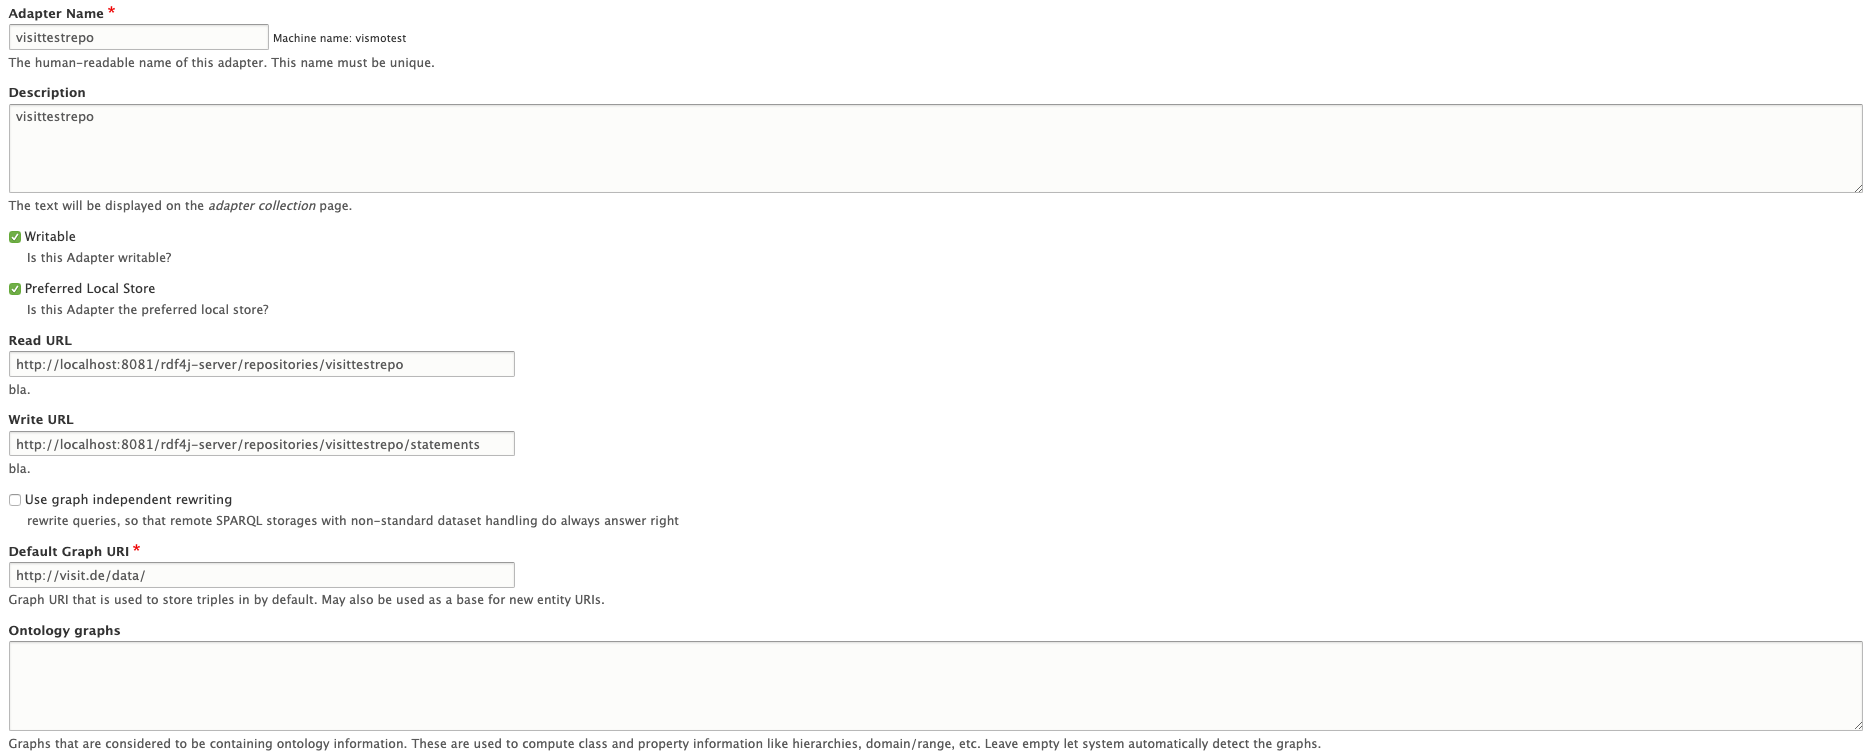
\includegraphics[width=1.0\textwidth,height=0.4\textwidth]{Figures/berndl/adapter1}
    \caption{\label{fig:adapter1} Übersicht der Konfiguration eines \wisski Salz Adapters, Teil 1.}
\end{sidewaysfigure}

\begin{sidewaysfigure}
    %\centering
    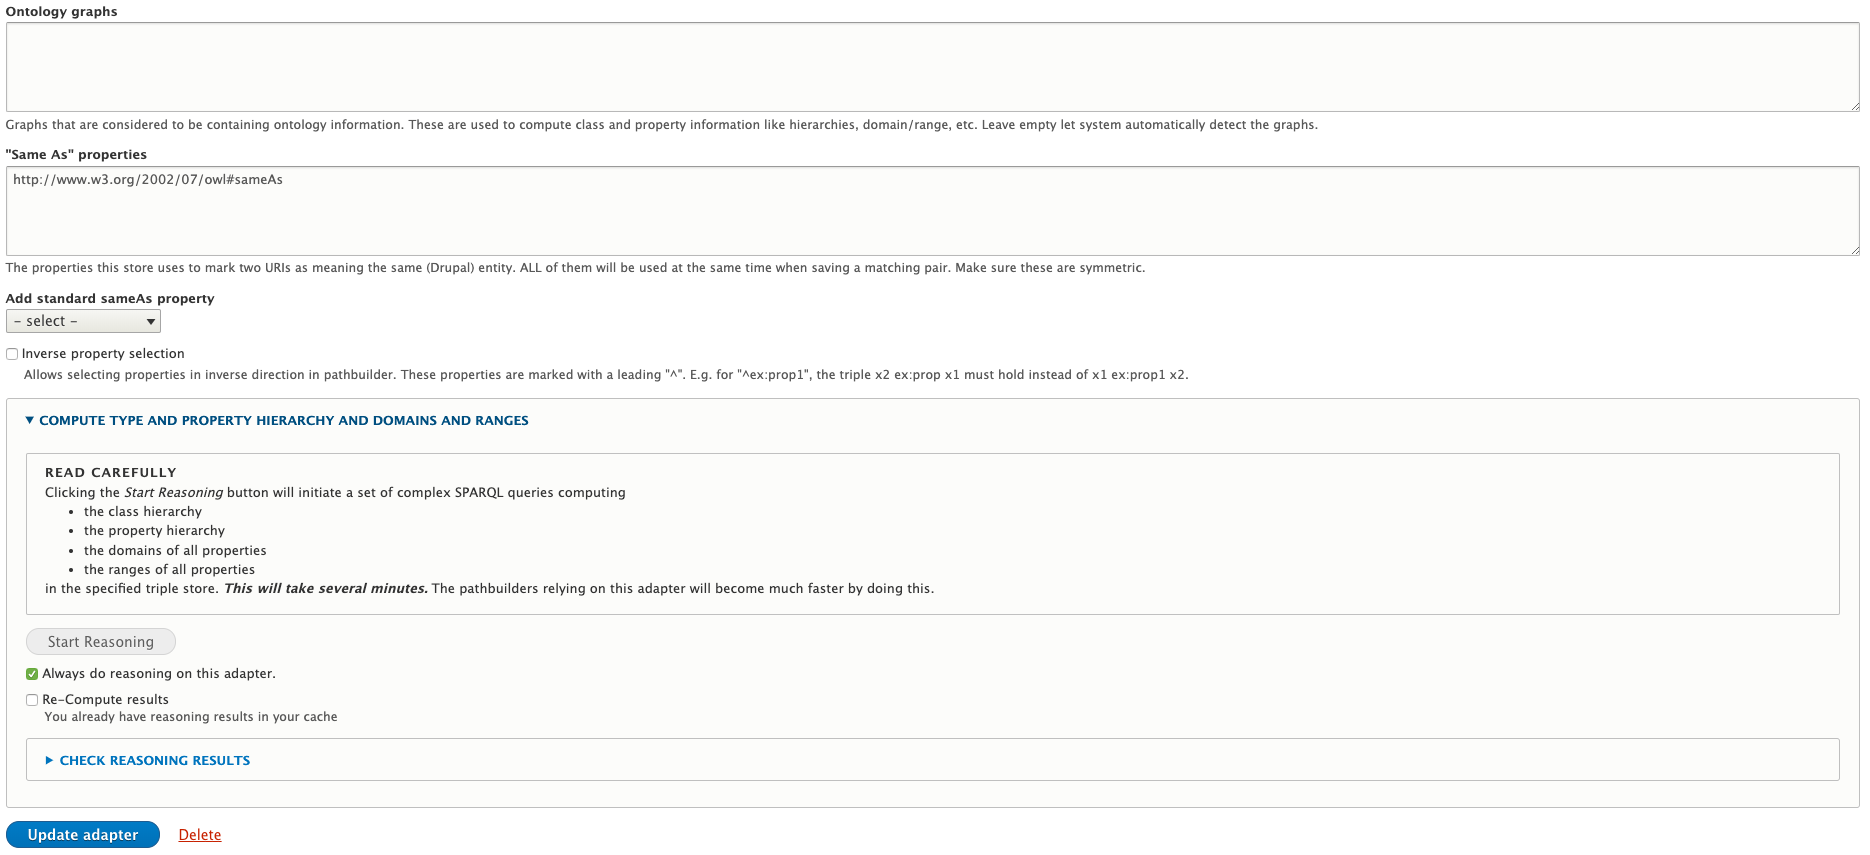
\includegraphics[width=1.0\textwidth,height=0.4\textwidth]{Figures/berndl/adapter3}
    \caption{\label{fig:adapter2} Übersicht der Konfiguration eines \wisski Salz Adapters, Teil 2.}
\end{sidewaysfigure}

\begin{sidewaysfigure}
    %\centering
    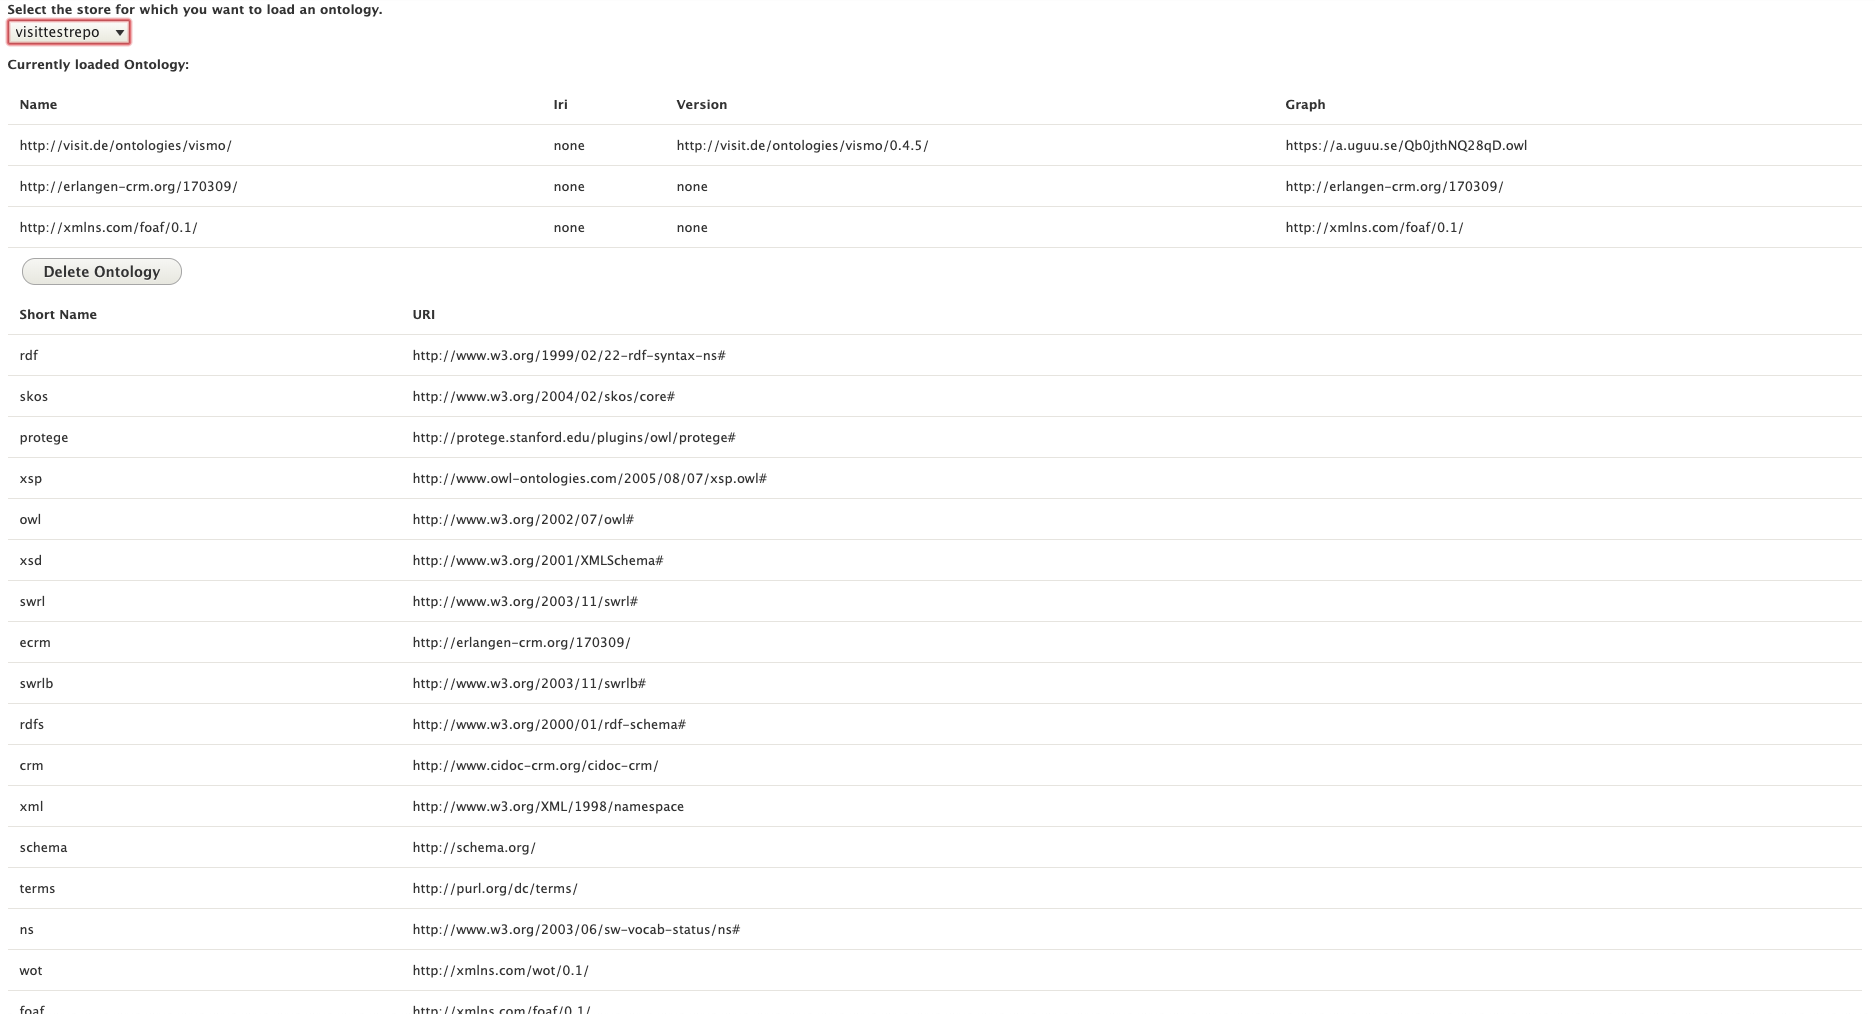
\includegraphics[width=1.0\textwidth,height=0.4\textwidth]{Figures/berndl/wisskiontology}
    \caption{\label{fig:wisskiontology} Detailansicht einer definierten Ontology im \wisski System am Beispiel VisMo für das ViSIT Projekt.}
\end{sidewaysfigure}

\begin{sidewaysfigure}
    %\centering
    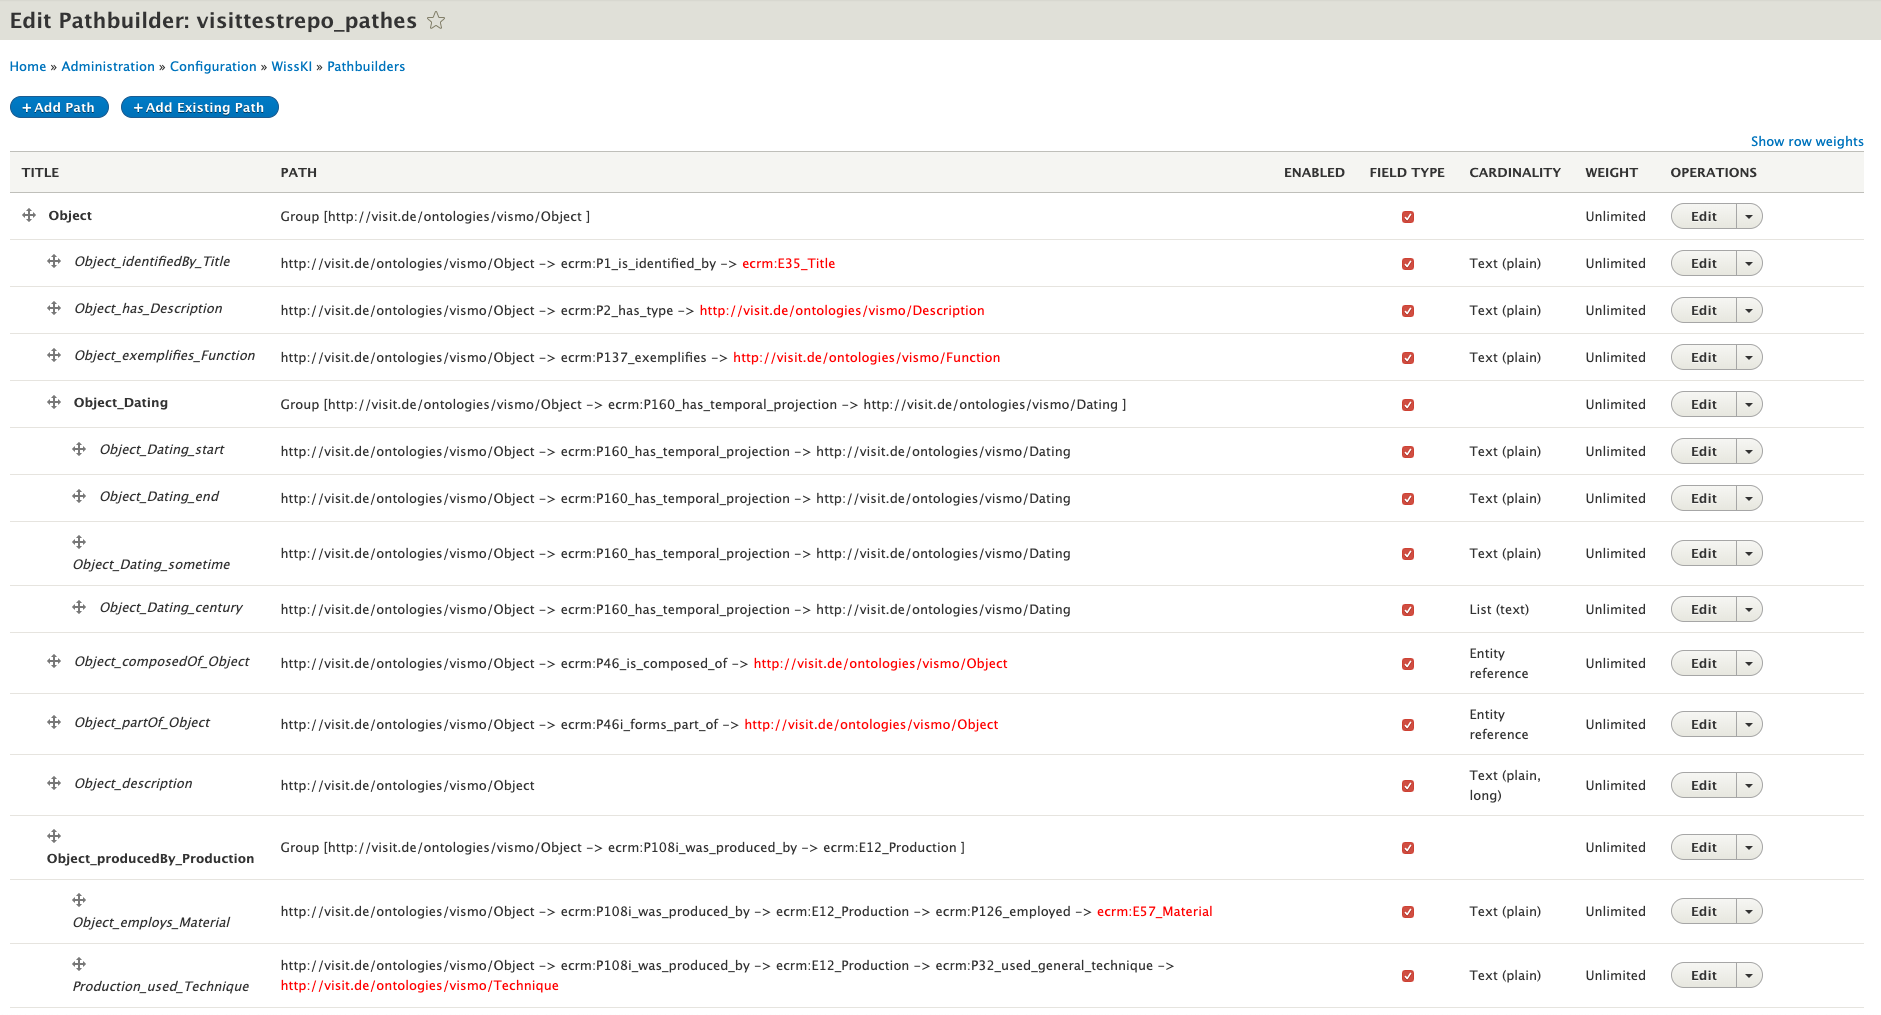
\includegraphics[width=1.0\textwidth,height=0.4\textwidth]{Figures/berndl/pathbuilder}
    \caption{\label{fig:pathbuilder} Übersicht der ersten Pfade des für das \visit Projekt definierten Pathbuilders.}
\end{sidewaysfigure}

\begin{figure}[htb]
    \centering
    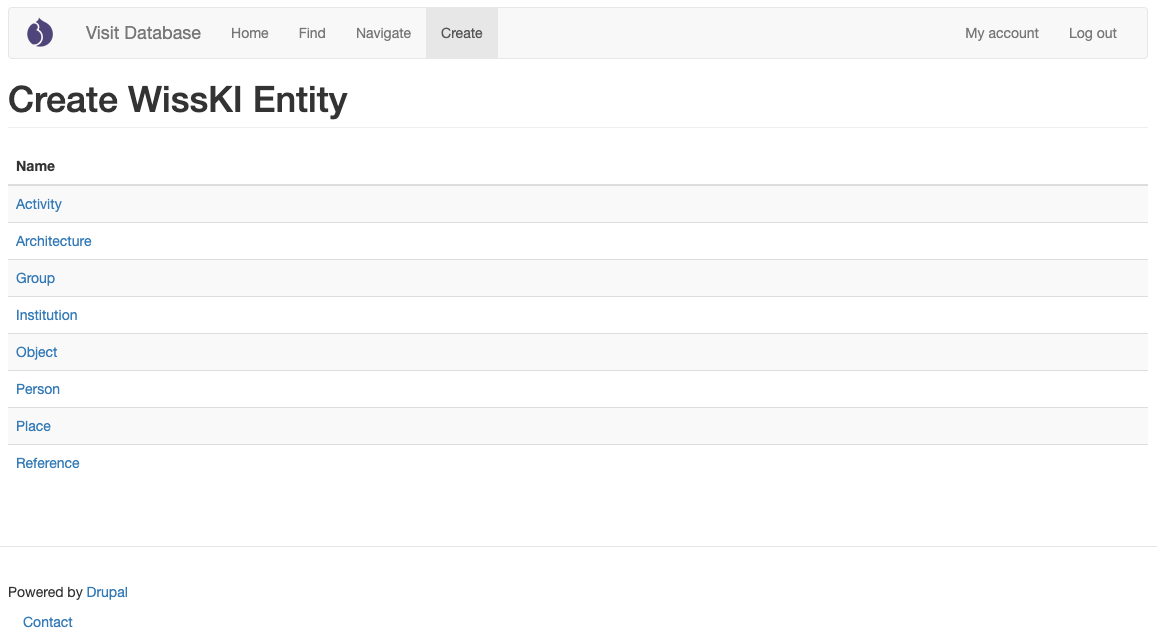
\includegraphics[width=\textwidth]{Figures/berndl/wisskiCreate}
    \caption{\label{fig:wisskiCreate} Ausgangs-Interface zum Erzeugen einer Hauptentität im \wisski System.}
\end{figure}

\begin{sidewaysfigure}
    %\centering
    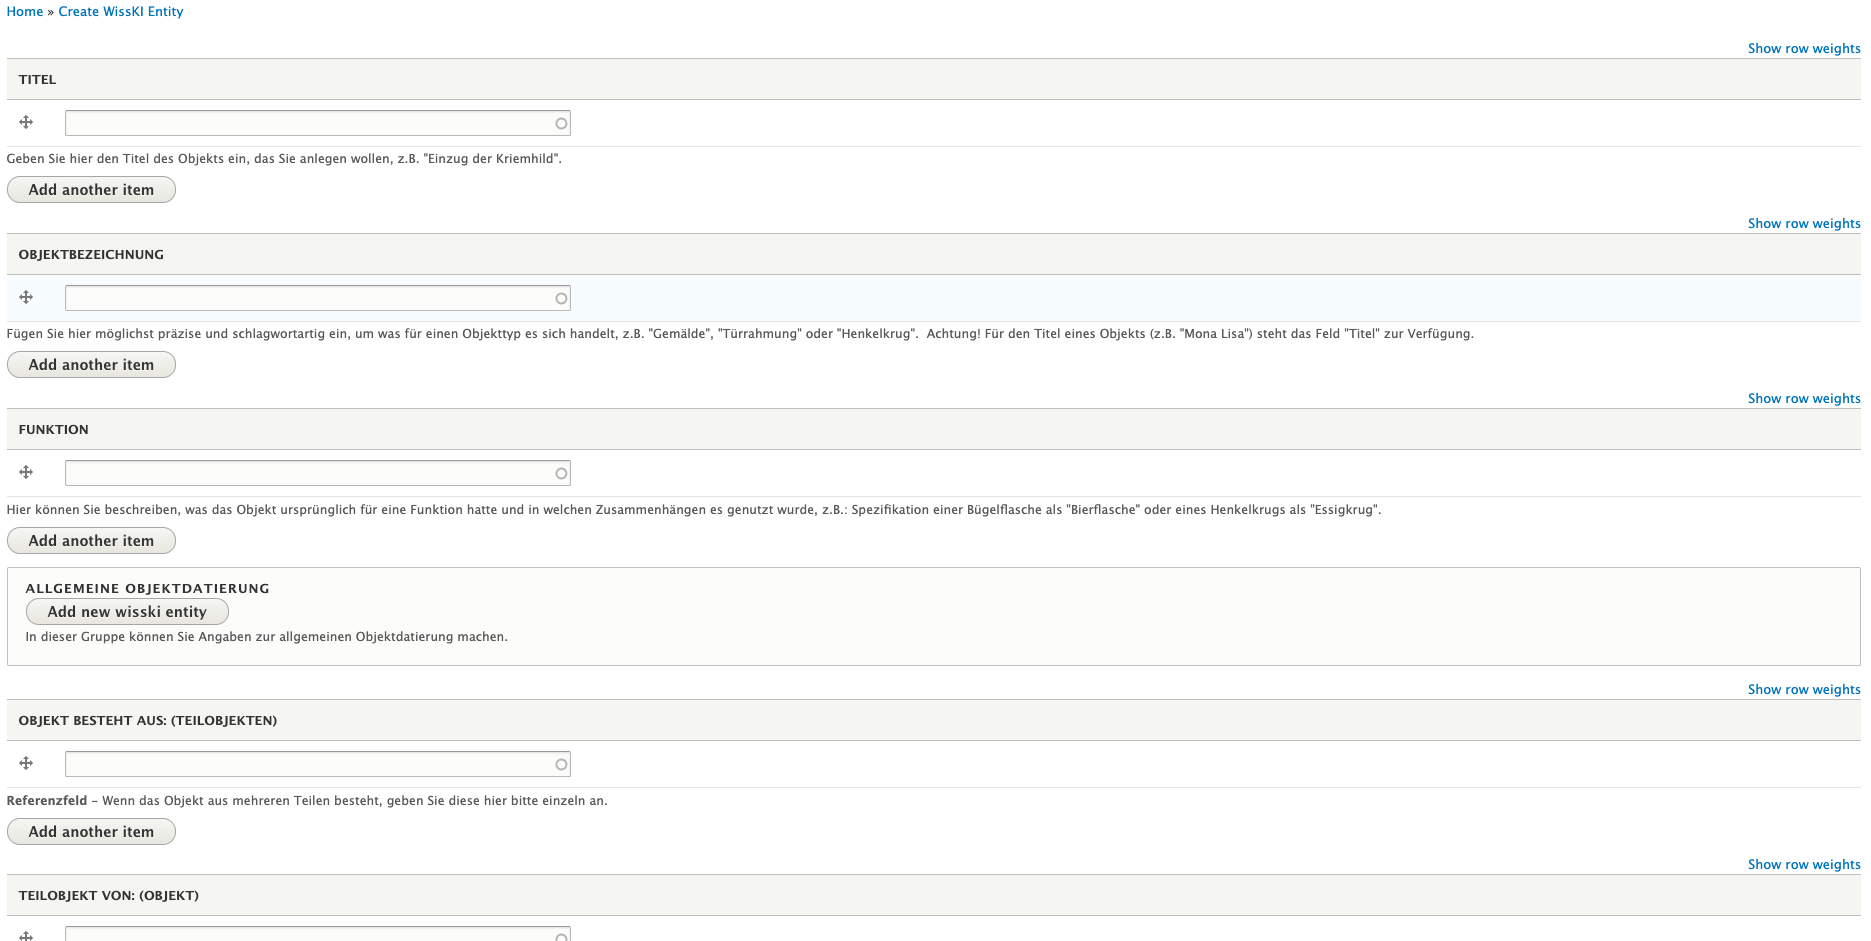
\includegraphics[width=1.0\textwidth,height=0.4\textwidth]{Figures/berndl/wisskiCreateObject}
    \caption{\label{fig:wisskiCreateObject} Eingabe-Interface für ein Ausstellungsobjekt im \visit \wisski System.}
\end{sidewaysfigure}

\begin{figure}[htb]
    \centering
    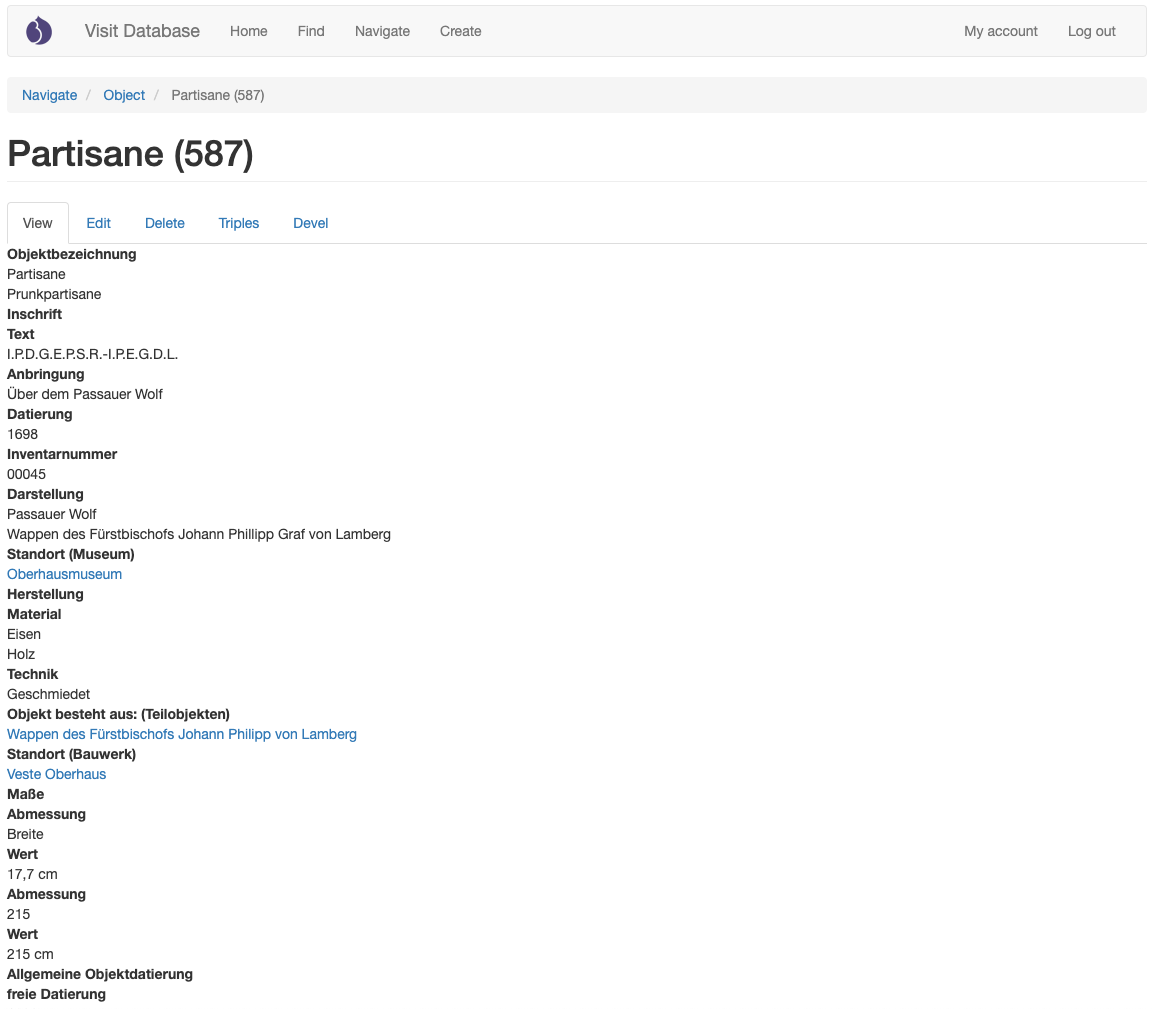
\includegraphics[width=\textwidth]{Figures/berndl/wisskiViewObject}
    \caption{\label{fig:wisskiViewObject} Beispiel Ausgabe-Interface einer Partisane des \visit \wisski Systems.}
\end{figure}

%----------------------------------------------------------------------------------------
%	BIBLIOGRAPHY
%----------------------------------------------------------------------------------------

\renewcommand{\refname}{\spacedlowsmallcaps{References}} % For modifying the bibliography heading

%\bibliographystyle{unsrt}

%\bibliography{Bibs/baumgaertner, Bibs/kufstein, Bibs/schlenker, Bibs/berndl2}% The file containing the bibliography

\printbibliography

%----------------------------------------------------------------------------------------

\end{document}